\documentclass[11pt]{article}
\usepackage[margin=0.78in]{geometry}
\usepackage[T1]{fontenc}
\usepackage{lmodern}
\usepackage{microtype}
\usepackage{amsmath,amssymb,amsthm,mathtools,bm}
\usepackage{booktabs,longtable,array,multirow}
\usepackage{pdflscape}
\usepackage{enumitem}
\usepackage{xcolor}
\usepackage{graphicx}
\usepackage{tikz}
\usetikzlibrary{arrows.meta,positioning,fit,calc,shapes.geometric,matrix}
\usepackage{xurl}
\usepackage{hyperref}
\usepackage[nameinlink,capitalise]{cleveref}
\usepackage{tcolorbox}
\tcbuselibrary{breakable,skins}
\usepackage{caption}
\hypersetup{colorlinks=true,linkcolor=blue,citecolor=blue!60!black,urlcolor=blue,pdftitle={Time-Residual Genesis of Gravity and the Four Fundamental Interactions - V22 Main Manuscript},pdfauthor={Seunghyun Hong},pdfsubject={Main manuscript: parent covariant residual field equation, time-residual dimensional genesis, gravity origin, and four-interaction unification}}
\captionsetup{labelfont={bf,color=blue},textfont={color=black}}
\setlength{\parindent}{1.2em}
\setlength{\parskip}{0.22em}
\setlist[itemize]{leftmargin=1.65em,itemsep=0.18em,topsep=0.28em}
\setlist[enumerate]{leftmargin=1.85em,itemsep=0.18em,topsep=0.28em}
\numberwithin{equation}{section}
\allowdisplaybreaks
\emergencystretch=2em
\pagestyle{plain}

\newtheorem{definition}{Definition}[section]
\newtheorem{axiom}[definition]{Axiom}
\newtheorem{lemma}[definition]{Lemma}
\newtheorem{theorem}[definition]{Theorem}
\newtheorem{proposition}[definition]{Proposition}
\newtheorem{corollary}[definition]{Corollary}
\newtheorem{protocol}[definition]{Protocol}
\theoremstyle{remark}
\newtheorem{remark}[definition]{Remark}

\newcommand{\R}{\mathbb{R}}
\newcommand{\Q}{\mathbb{Q}}
\newcommand{\N}{\mathbb{N}}
\newcommand{\Id}{\mathrm{Id}}
\newcommand{\sgn}{\operatorname{sgn}}
\newcommand{\rank}{\operatorname{rank}}
\newcommand{\tr}{\operatorname{tr}}
\newcommand{\diag}{\operatorname{diag}}
\newcommand{\im}{\operatorname{im}}
\newcommand{\kerp}{\operatorname{ker}}
\newcommand{\CRGE}{\textsc{crge}}
\newcommand{\DGPC}{\textsc{dgpc}}
\newcommand{\Hsrc}{\mathcal H_{\mathrm{src}}}
\newcommand{\Hsh}{\mathcal H_{\mathrm{sh}}}
\newcommand{\Asrc}{\mathcal A_{\mathrm{src}}}
\newcommand{\Ash}{\mathcal A_{\mathrm{sh}}}
\newcommand{\Pg}{P_{\mathrm G}}
\newcommand{\Pe}{P_{\mathrm E}}
\newcommand{\Pw}{P_{\mathrm W}}
\newcommand{\Ps}{P_{\mathrm S}}

\definecolor{ledgerblue}{RGB}{5,5,150}
\definecolor{ledgergray}{RGB}{88,88,88}
\definecolor{ledgergreen}{RGB}{0,122,0}
\definecolor{ledgerback}{RGB}{247,247,255}
\newtcolorbox{blueledger}[1]{enhanced,breakable,colback=ledgerback,colframe=ledgerblue,colbacktitle=ledgerblue,coltitle=white,fonttitle=\bfseries,title={#1},boxrule=0.9pt,arc=2mm,left=4mm,right=4mm,top=2mm,bottom=2mm,before skip=2mm,after skip=3mm}
\newtcolorbox{grayledger}[1]{enhanced,breakable,colback=gray!5,colframe=ledgergray,colbacktitle=ledgergray,coltitle=white,fonttitle=\bfseries,title={#1},boxrule=0.9pt,arc=2mm,left=4mm,right=4mm,top=2mm,bottom=2mm,before skip=2mm,after skip=3mm}
\newtcolorbox{greenledger}[1]{enhanced,breakable,colback=green!3,colframe=ledgergreen,colbacktitle=ledgergreen,coltitle=white,fonttitle=\bfseries,title={#1},boxrule=0.9pt,arc=2mm,left=4mm,right=4mm,top=2mm,bottom=2mm,before skip=2mm,after skip=3mm}
\newtcolorbox{interpretivebridge}[1]{enhanced,breakable,colback=cyan!3,colframe=blue!65!black,colbacktitle=blue!65!black,coltitle=white,fonttitle=\bfseries,title={Interpretive bridge: #1},boxrule=0.8pt,arc=2mm,left=4mm,right=4mm,top=2mm,bottom=2mm,before skip=2mm,after skip=3mm}
\newtcolorbox{conceptledger}[1]{enhanced,breakable,colback=yellow!4,colframe=orange!70!black,colbacktitle=orange!70!black,coltitle=white,fonttitle=\bfseries,title={Conceptual interpretation: #1},boxrule=0.85pt,arc=2mm,left=4mm,right=4mm,top=2mm,bottom=2mm,before skip=2mm,after skip=3mm}
\newtcolorbox{proofguide}[1]{enhanced,breakable,colback=violet!2,colframe=violet!65!black,colbacktitle=violet!65!black,coltitle=white,fonttitle=\bfseries,title={Reader guide before the proof: #1},boxrule=0.75pt,arc=1.5mm,left=3mm,right=3mm,top=1.5mm,bottom=1.5mm,before skip=1.5mm,after skip=2mm}
\newtcolorbox{equationledger}[1]{enhanced,breakable,colback=teal!2,colframe=teal!65!black,colbacktitle=teal!65!black,coltitle=white,fonttitle=\bfseries,title={Generated effective equation: #1},boxrule=0.8pt,arc=2mm,left=4mm,right=4mm,top=2mm,bottom=2mm,before skip=2mm,after skip=3mm}
\newtcolorbox{centralformula}[1]{enhanced,breakable,colback=blue!2,colframe=blue!80!black,colbacktitle=blue!80!black,coltitle=white,fonttitle=\bfseries\large,title={#1},boxrule=1.1pt,arc=2mm,left=5mm,right=5mm,top=3mm,bottom=3mm,before skip=3mm,after skip=4mm}
\newcommand{\codefn}[1]{\texttt{\detokenize{#1}}}
\newcommand{\doi}[1]{\href{https://doi.org/#1}{#1}}


\begin{document}

\begin{center}
\vspace*{0.42cm}
{\Large\bfseries Time-Residual Genesis of Gravity and the Four Fundamental Interactions:\\[2mm]
The Parent Covariant Residual Field Equation from an Eighteen-State Relational Grammar\par}
\vspace{0.78cm}
{\large Seunghyun Hong\par}
Independent Researcher, Republic of Korea\\
ORCID: 0009-0000-4044-2565\\
Correspondence: \href{mailto:madein7504@naver.com}{madein7504@naver.com}\\
Archival manuscript: V22 - Main Manuscript\\
Zenodo record DOI: \doi{10.5281/zenodo.21702095}\\
Zenodo all-versions DOI: \doi{10.5281/zenodo.21127052}\\
\vspace{0.60cm}
\end{center}

\begin{blueledger}{Dependency-ordered unified proof}
The proof begins with the negative--zero--positive relational grammar and its occupied/vacant inner states. Directed transition generates time; temporal residuals generate spatial rank three; the JS shell generates the source carrier; and one complete parent grammar is decomposed by intrinsic conditional expectations rather than by a choice among competing force paths. The anonymous nonconstant blocks have ranks $5$, $1$, $3$, and $8$. A generated sector-spectral edge operator and one parent covariant residual field equation then transport the complete carrier. Its gravitational projection generates the finite temporal-scale correlation, its closed-path transport generates parent curvature, and one physical parent action generates the four field projections and the matter equation.
\end{blueledger}

\begin{blueledger}{Reading rule for boxes and formal proofs}
Boxes contain only interpretation, notation, physical meaning, dependency information, or guidance for the reader. Definitions, lemmas, theorems, equations, calculations, and proofs are written in the ordinary unboxed article format immediately after the corresponding guide. No formal derivation is hidden inside a colored box.
\end{blueledger}

\begin{abstract}
A self-contained four-interaction construction is presented in one dependency order from a finite relational grammar to temporal order, residual dimensional genesis, a canonical force carrier, a logarithm-free covariant residual dynamics, metric gravity, compact internal curvature, one parent action, chiral matter, ratio observables, and compatible continuum descendants. The primitive alphabet is the product of an outer negative-zero-positive relation, an inner A-B-C relation carrying negative-zero-positive orientation, and independent occupied-vacant complementarity. It has exactly eighteen states, including occupied and vacant negative, zero, and positive inner states inside each outer negative, zero, and positive sector. Directed minimal transition generates one temporal order. The outer-sign, inner-relation, and occupancy differences along this order generate three independent temporal residuals; their span is the minimal spatial carrier of rank three. The twelve signed two-axis residual directions form a closed JS shell with exact incidence and a refinement anisotropy spread of $2/(9N)$.

Uniform conditional expectations of the three primitive factors generate the complete orthogonal interaction-order decomposition. Removing the constant mode and splitting the fully centered block produces the anonymous nonconstant ranks $5+1+3+8=17$. Exact matrix operations realize the five-dimensional symmetric tracefree spin-two response, a one-dimensional anti-Hermitian center, a three-dimensional compact algebra, and the traceless anti-Hermitian three-by-three algebra. Closure, Jacobi identities, invariant forms, representation action, charge-nullspace constraints, and anomaly cancellation are checked before measured coupling or mass values are admitted.

The central dynamical theorem is the parent covariant residual field equation. For the exact residual coordinate $\mathcal R(X)=(I-X)X^{-1}$,
\[
\mathcal R(X_q)=\mathbb A_{pq}U_{pq}\mathcal R(X_p)U_{pq}^{-1},
\qquad
\mathbb A_{pq}=\sum_i a_i(p,q)P_i.
\]
The generated sector-spectral operator satisfies identity, reversal, and path composition. The target residual and bounded shadow exist constructively and are unique; positive residual blocks remain positive and the target shadow remains strictly inside the spectral interval $(0,1)$. The full matrix equation is covariant under independent endpoint-frame transformations and defines an exact path groupoid. Its gravitational projection gives a finite target-over-source temporal-scale correlation. The differential coefficient $dN/N$ is derived from the finite identity and is not supplied by an evaluated logarithm. Its internal noncommuting transport gives plaquette holonomy; rational polynomial coefficient extraction yields the commutator term, and link variation yields one parent curvature.

The residual consistency functional is a nonnegative certificate and is not varied as a fifth interaction. The sole physical variational object is
\[
S_{\rm parent}[\Omega,\Psi]
=\frac12\langle\mathcal F_\Omega,\mathbb M\mathcal F_\Omega\rangle
+\langle\bar\Psi,\mathcal D_\Omega\Psi\rangle+V_{\rm rad}(\Psi).
\]
One connection variation yields four orthogonal field projections, and the independent matter variation yields the matter equation. Chiral charge ratios, exact anomaly cancellation, three temporal generations, mixing, finite path amplitudes, normalized branching packets, rational scattering, ratio flow, continuum completion, and thirty effective equation descents are generated through the same middle gate. The executable source has 66,229 lines and produces a deterministic output of 1,824,059 lines. It executes 487 primary and 38 narrative roots, 525 in total, with 544 explicit derivations, exit code zero, and an empty error stream. The result is internal closure on the declared generated classes; empirical identity, unrestricted equivalence, historical priority, and third-party reproduction remain external tests.
\end{abstract}

\noindent\textbf{Keywords:} temporal residual; dimensional genesis; structured zero; occupied and vacant states; canonical $5+1+3+8$ decomposition; parent covariant residual field equation; finite gravity correlation; holonomy; parent action; four-interaction unification.

\tableofcontents
\clearpage
\section*{Complete causal proof maps}
\addcontentsline{toc}{section}{Complete causal proof maps}
\begin{figure}[htbp]
\centering
\resizebox{0.88\textwidth}{!}{%
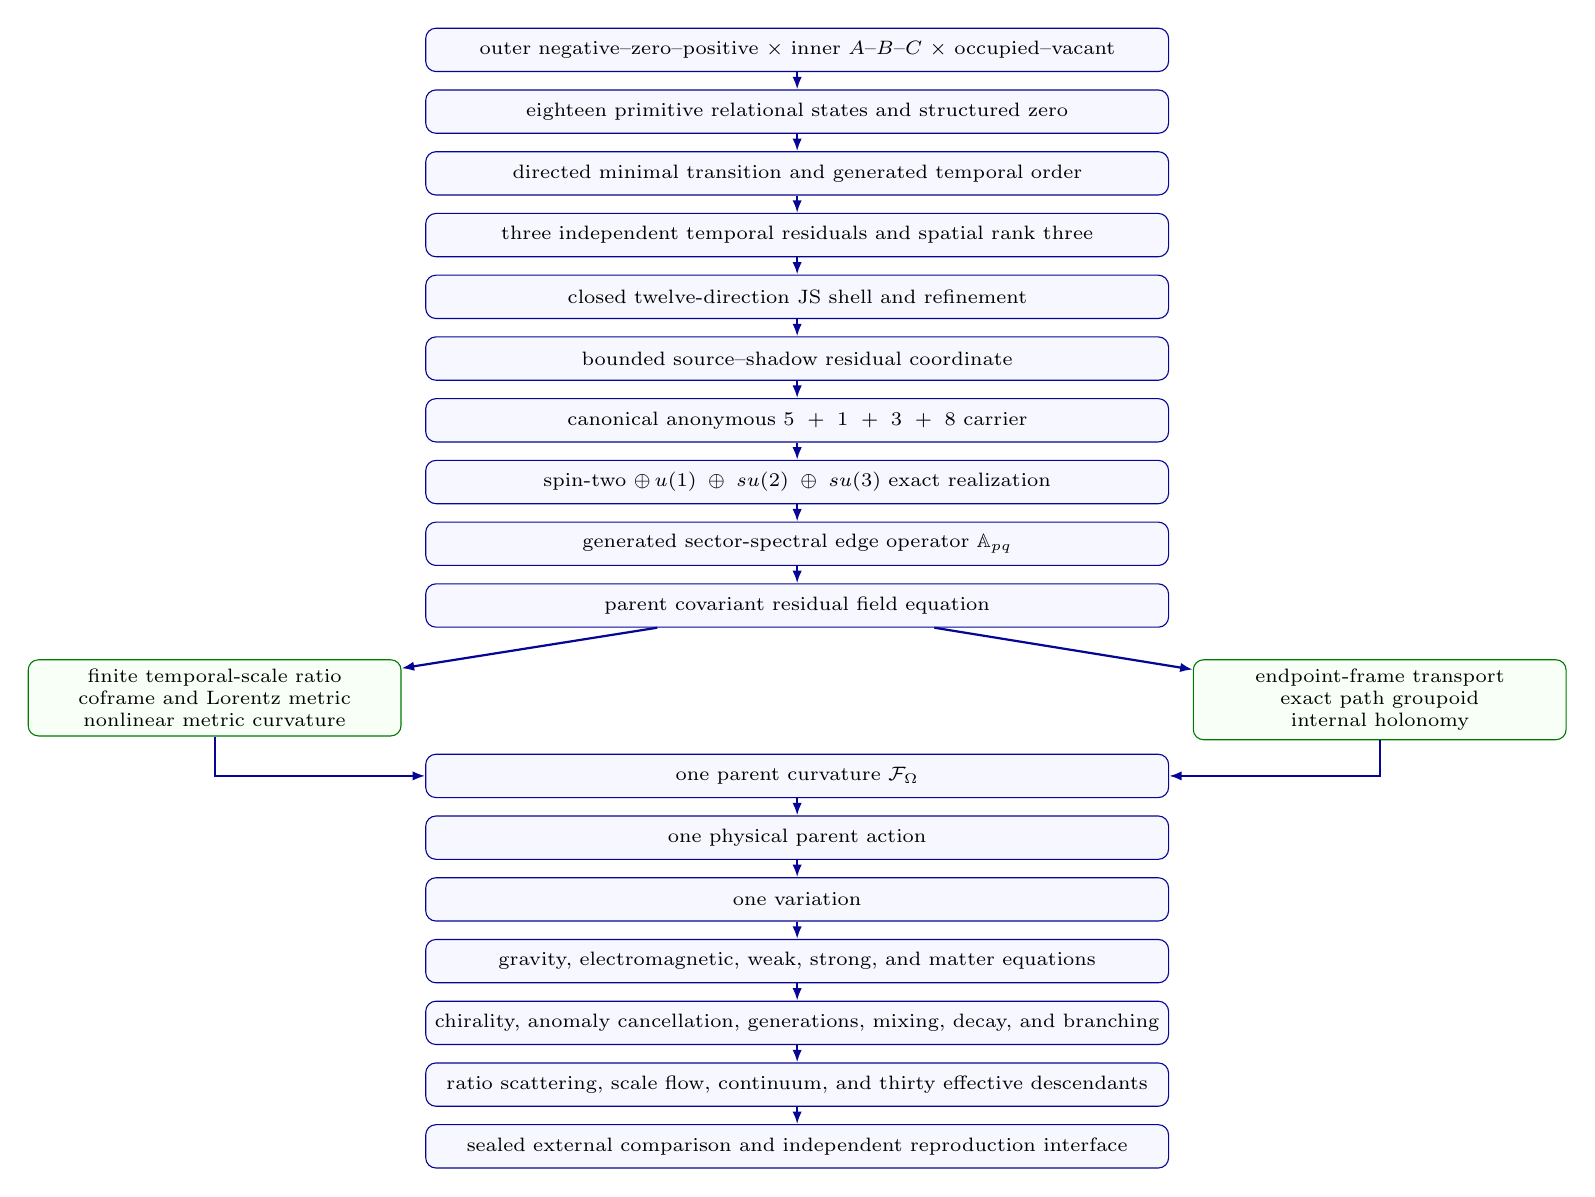
\begin{tikzpicture}[node distance=2.2mm,box/.style={draw=ledgerblue,rounded corners=1.3mm,fill=blue!3,minimum height=5.5mm,text width=9.2cm,align=center,font=\scriptsize},split/.style={draw=ledgergreen,rounded corners=1.3mm,fill=green!3,minimum height=8mm,text width=4.5cm,align=center,font=\scriptsize},arr/.style={-{Latex[length=1.6mm]},thick,draw=ledgerblue}]
\node[box] (a0) {outer negative--zero--positive $\times$ inner $A$--$B$--$C$ $\times$ occupied--vacant};
\node[box,below=of a0] (a1) {eighteen primitive relational states and structured zero};
\node[box,below=of a1] (a2) {directed minimal transition and generated temporal order};
\node[box,below=of a2] (a3) {three independent temporal residuals and spatial rank three};
\node[box,below=of a3] (a4) {closed twelve-direction JS shell and refinement};
\node[box,below=of a4] (a5) {bounded source--shadow residual coordinate};
\node[box,below=of a5] (a6) {canonical anonymous $5+1+3+8$ carrier};
\node[box,below=of a6] (a7) {spin-two $\oplus\,u(1)\oplus su(2)\oplus su(3)$ exact realization};
\node[box,below=of a7] (a8) {generated sector-spectral edge operator $\mathbb A_{pq}$};
\node[box,below=of a8] (a9) {parent covariant residual field equation};
\node[split,below left=4mm and 3mm of a9] (g) {finite temporal-scale ratio\\coframe and Lorentz metric\\nonlinear metric curvature};
\node[split,below right=4mm and 3mm of a9] (i) {endpoint-frame transport\\exact path groupoid\\internal holonomy};
\node[box,below=16mm of a9] (a10) {one parent curvature $\mathcal F_\Omega$};
\node[box,below=of a10] (a11) {one physical parent action};
\node[box,below=of a11] (a12) {one variation};
\node[box,below=of a12] (a13) {gravity, electromagnetic, weak, strong, and matter equations};
\node[box,below=of a13] (a14) {chirality, anomaly cancellation, generations, mixing, decay, and branching};
\node[box,below=of a14] (a15) {ratio scattering, scale flow, continuum, and thirty effective descendants};
\node[box,below=of a15] (a16) {sealed external comparison and independent reproduction interface};
\foreach \u/\v in {a0/a1,a1/a2,a2/a3,a3/a4,a4/a5,a5/a6,a6/a7,a7/a8,a8/a9,a10/a11,a11/a12,a12/a13,a13/a14,a14/a15,a15/a16}{\draw[arr] (\u)--(\v);}
\draw[arr] (a9)--(g); \draw[arr] (a9)--(i); \draw[arr] (g.south) |- (a10.west); \draw[arr] (i.south) |- (a10.east);
\end{tikzpicture}%
}
\caption{Authoritative causal proof map generated from the standalone dependency spine. The central residual equation occurs after the primitive grammar, temporal residual space, JS shell, canonical carrier, exact algebra, and generated edge spectrum. Gravity and internal holonomy are two descendants of the same finite middle law and enter one parent curvature and one physical action.}
\label{fig:causal}
\end{figure}

\clearpage
\begin{figure}[htbp]
\centering
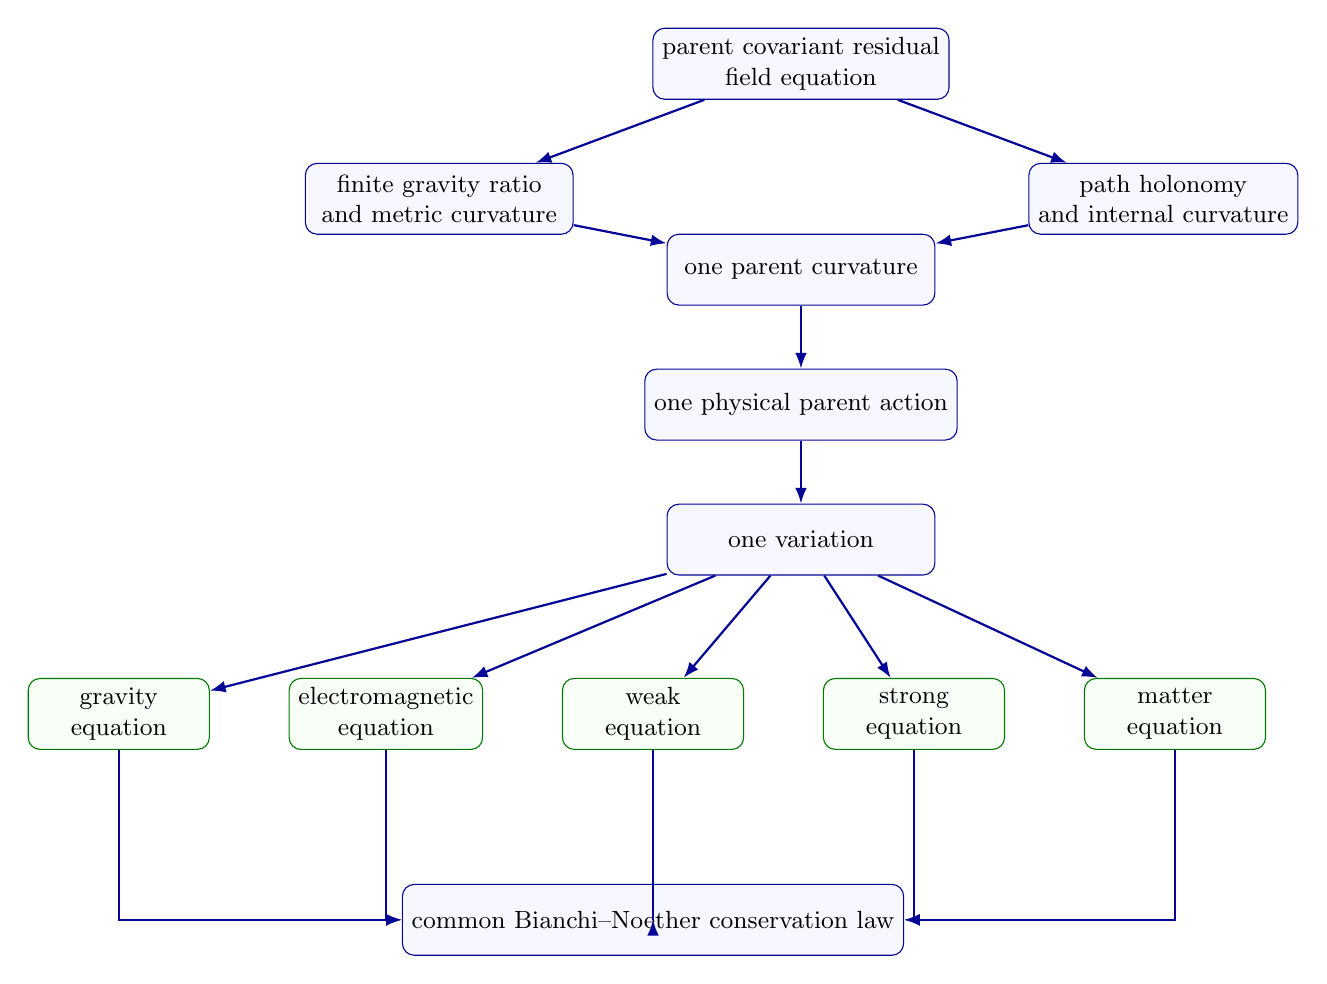
\begin{tikzpicture}[node distance=8mm and 10mm,box/.style={draw=ledgerblue,rounded corners=1.5mm,fill=blue!3,minimum width=3.4cm,minimum height=9mm,align=center,font=\small},force/.style={draw=ledgergreen,rounded corners=1.5mm,fill=green!3,minimum width=2.3cm,minimum height=9mm,align=center,font=\small},arr/.style={-{Latex[length=2mm]},thick,draw=ledgerblue}]
\node[box] (R) {parent covariant residual\\field equation};
\node[box,below left=of R] (G0) {finite gravity ratio\\and metric curvature};
\node[box,below right=of R] (H0) {path holonomy\\and internal curvature};
\node[box,below=17mm of R] (F) {one parent curvature};
\node[box,below=of F] (S) {one physical parent action};
\node[box,below=of S] (V) {one variation};
\node[force,below left=13mm and 58mm of V] (G) {gravity\\equation};
\node[force,right=of G] (E) {electromagnetic\\equation};
\node[force,right=of E] (W) {weak\\equation};
\node[force,right=of W] (C) {strong\\equation};
\node[force,right=of C] (M) {matter\\equation};
\node[box,below=17mm of W] (B) {common Bianchi--Noether conservation law};
\draw[arr] (R)--(G0); \draw[arr] (R)--(H0); \draw[arr] (G0)--(F); \draw[arr] (H0)--(F); \draw[arr] (F)--(S); \draw[arr] (S)--(V);
\foreach \x in {G,E,W,C,M}{\draw[arr] (V)--(\x); \draw[arr] (\x) |- (B);}
\end{tikzpicture}
\caption{Residual-to-variation structure. The nonnegative residual consistency functional is not a second action and does not appear in this physical variation diagram.}
\label{fig:variation}
\end{figure}
\clearpage


\section*{Notation, object types, and input--output rules}
\addcontentsline{toc}{section}{Notation, object types, and input--output rules}

\begin{interpretivebridge}{why a complete symbol dictionary is required}
The central equations are operator equations, not ordinary scalar formulas into which arbitrary measured numbers are inserted. A reader must know the type, dimension, domain, construction rule, and input--output role of every symbol before attempting a calculation. The tables below give that information before the compact equation map is displayed.
\end{interpretivebridge}

\subsection*{General algebraic conventions}
All finite primitive counts and ratio calculations use exact integers or rational numbers. Matrix-valued quantities act on the generated seventeen-dimensional nonconstant carrier unless a smaller projected block is explicitly indicated. The symbols $p$ and $q$ denote the initial and terminal vertices of an oriented generated edge; in a depth-labelled realization, $q-p$ is the integer depth increment. The symbol $I_n$ is the identity on an $n$-dimensional carrier, $X^{-1}$ denotes an inverse on the stated admissible domain, $\oplus$ denotes an orthogonal direct sum, and $\langle\cdot,\cdot\rangle$ denotes the generated invariant inner product or its spacetime-integrated extension.

\begin{longtable}{p{2.1cm}p{3.1cm}p{3.2cm}p{5.6cm}}
\toprule
Symbol & Name & Mathematical type & Meaning, construction, and use\\
\midrule\endhead
$\mathcal A$ & primitive relational alphabet & finite set of size $18$ & The product of outer sign, inner relation, and occupancy. It is generated before time or space and is not a fitted data table.\\
$\Sigma_{\rm out}$ & outer relation set & $\{-1,0,+1\}$ & Negative, balanced, and positive comparison of the selected whole with an exterior reference.\\
$\Sigma_{\rm in}$ & inner relation set & $\{A,B,C\}$ & Inner negative, zero, and positive roles, encoded by $A\mapsto-1$, $B\mapsto0$, $C\mapsto+1$.\\
$\Omega_{\rm occ}$ & occupancy set & $\{0,1\}$ & Vacant and occupied status, independent of the relational sign.\\
$\chi_{\rm out},\chi_{\rm in},\chi_{\rm occ}$ & primitive characters & scalar functions on $\mathcal A$ & Exact numerical readouts of outer orientation, inner orientation, and centered occupancy.\\
$\Delta\chi$ & temporal residual vector & vector in $\Q^3$ & The ordered difference of the three primitive characters across one directed update.\\
$\mathcal H_{18}$ & complete parent function space & $18$-dimensional inner-product space & All real functions on the eighteen primitive states.\\
$\mathcal H_0$ & constant mode & rank-$1$ subspace & The uniform function removed before the nonconstant interaction carrier is formed.\\
$\mathcal H_5$ & metric-response block & rank-$5$ subspace & Symmetric tracefree spatial response, identified with the gravity role only after its operational signature is proved.\\
$\mathcal H_1$ & central internal block & rank-$1$ subspace & One-dimensional anti-Hermitian center, identified with the electromagnetic role.\\
$\mathcal H_3$ & two-state compact block & rank-$3$ subspace & Exact compact three-generator algebra with the weak operational signature.\\
$\mathcal H_8$ & three-state traceless compact block & rank-$8$ subspace & Exact traceless anti-Hermitian $3\times3$ algebra with the strong operational signature.\\
$P_{\rm G},P_{\rm E},P_{\rm W},P_{\rm S}$ & canonical projectors & $17\times17$ idempotent operators & Orthogonal projections onto ranks $5,1,3,8$. They are generated by conditional expectations, not inserted as force labels.\\
$\lambda_i$ & generated sector response ratio & positive rational scalar & The normalized response spectrum $(153,68,108,180)/509$ in the order E, W, S, G. These are internal dimensionless ratios, not measured coupling constants.\\
$X_p$ & source bounded shadow & positive $17\times17$ operator & The state at edge origin $p$, with spectrum strictly inside $(0,1)$. It is an admissible initial condition or a result of an earlier edge update.\\
$\mathcal R(X)$ & exact residual coordinate & matrix function & $\mathcal R(X)=(I-X)X^{-1}$. It maps a bounded shadow bijectively to a positive residual.\\
$R_p,R_q$ & source and target residuals & positive operators & Abbreviations for $\mathcal R(X_p)$ and $\mathcal R(X_q)$. The target is calculated, not inserted.\\
$a_i(p,q)$ & sector edge multiplier & positive rational scalar & The finite response multiplier on sector $i$ across edge $p\to q$.\\
$N(p)$ & local temporal scale & positive scalar & Generated local clock-scale factor at $p$. Only the ratio $N(q)/N(p)$ enters the primitive finite gravity relation.\\
$\mathbb A_{pq}$ & sector-spectral edge operator & positive block-scalar $17\times17$ operator & $\sum_i a_i(p,q)P_i$. It supplies finite compression while preserving the canonical decomposition.\\
$U_{pq}$ & parent frame transport & invertible block-preserving operator & Carries a source frame at $p$ to the target frame at $q$. In exact finite examples it is constructed by rational Cayley transforms.\\
$R_{\rm G}$ & gravitational residual block & operator on $\mathcal H_5$ & The $P_{\rm G}$ projection of the complete residual.\\
$R_{\rm G}^{U}(p)$ & transported source gravity residual & operator on $\mathcal H_5$ & $U_{{\rm G},pq}R_{\rm G}(p)U_{{\rm G},pq}^{-1}$.\\
$\Delta N$ & finite clock-scale increment & scalar & $N(q)-N(p)$. It is used before any differential limit.\\
$H_{\square}$ & plaquette holonomy & invertible matrix & Ordered product of four rational link transports around one elementary closed path.\\
$\epsilon$ & formal expansion parameter & indeterminate & A coefficient-bookkeeping symbol in $\Q[\epsilon]/(\epsilon^3)$, not an experimentally fitted small number.\\
$[Y,X]$ & commutator & matrix & $YX-XY$ under the convention used in the plaquette expansion.\\
$\Omega$ & parent connection & matrix-valued one-form & Local generator of parent frame transport on the generated carrier.\\
$\mathcal F_{\Omega}$ & parent curvature & matrix-valued two-form & $d\Omega+\Omega\wedge\Omega$, obtained from link variation and noncommuting holonomy.\\
$\mathbb M$ & response metric & positive block-diagonal operator & Weights the curvature sectors in the single parent action and is diagonal on the canonical projectors.\\
$\Psi$ & parent matter field & section of generated matter representation & Contains the chiral matter components after the force carrier has been generated.\\
$\bar\Psi$ & conjugate matter field & dual section & The appropriate adjoint or conjugate variable varied independently in the matter Euler--Lagrange equation.\\
$\mathcal D_{\Omega}$ & covariant matter operator & first-order differential operator & The generated matter operator coupled to the parent connection.\\
$V_{\rm rad}(\Psi)$ & radial matter potential & gauge-invariant scalar functional & The generated radial/self-interaction contribution in the matter sector.\\
$S_{\rm parent}$ & physical parent action & scalar functional & The sole physical variational object. Its connection variation yields the four projected field equations; its matter variation yields the matter equation.\\
$C_{\rm res}$ & residual consistency functional & nonnegative scalar & A certificate that the finite middle equation holds on every edge. It is not varied and does not define a fifth force.\\
\bottomrule
\end{longtable}

\subsection*{Which quantities are supplied, generated, and returned?}
For one edge update, the independent supplied data are an admissible source state $X_p$, an oriented edge $p\to q$, and the generated frame/link data appropriate to that edge. The projectors, response ratios, and block structure are fixed by earlier theorems. The edge operator $\mathbb A_{pq}$ and transport $U_{pq}$ are then constructed. The central equation returns one and only one target residual $R_q$ and one and only one target shadow $X_q$.

\begin{center}
\begin{tabular}{p{3.2cm}p{10.8cm}}
\toprule
Role & Objects\\
\midrule
Supplied at the edge & $p,q$, an admissible $X_p$, and the generated local link/frame data\\
Already fixed by earlier proofs & $P_i$, $\lambda_i$, the carrier dimensions, the inner products, and the admissible domains\\
Constructed for the edge & $a_i(p,q)$, $\mathbb A_{pq}$, $U_{pq}$, and $R_p=\mathcal R(X_p)$\\
Returned by the equation & $R_q$ and $X_q=(I+R_q)^{-1}$\\
Not inserted & measured coupling constants, measured particle masses, or a desired target value $X_q$\\
\bottomrule
\end{tabular}
\end{center}

\subsection*{Worked scalar reduction}
The matrix equation contains a simple one-sector example. Set $p=0$, $q=1$, choose the electromagnetic block, take $U_{pq}=1$, and choose $X_p=1/2$. Then
\begin{align}
R_p&=\frac{1-X_p}{X_p}=1,\\
a_{\rm E}(0,1)&=\lambda_{\rm E}=\frac{153}{509},\\
R_q&=a_{\rm E}(0,1)R_p=\frac{153}{509},\\
X_q&=\frac{1}{1+R_q}=\frac{509}{662}.
\end{align}
The input is the source state and the selected generated edge. The target $X_q$ is the output; it is not chosen in advance.

\subsection*{Worked four-block diagonal reduction}
Let the source residual be block diagonal,
\begin{equation}
R_p=r_{\rm G}P_{\rm G}+r_{\rm E}P_{\rm E}+r_{\rm W}P_{\rm W}+r_{\rm S}P_{\rm S},
\end{equation}
and let $U_{pq}=I$. Orthogonality gives
\begin{equation}
R_q=a_{\rm G}r_{\rm G}P_{\rm G}+a_{\rm E}r_{\rm E}P_{\rm E}+a_{\rm W}r_{\rm W}P_{\rm W}+a_{\rm S}r_{\rm S}P_{\rm S}.
\end{equation}
Thus the four components are not four independently postulated equations; they are the four canonical projections of one parent update.

\clearpage

\section*{Central equations of the theory}
\addcontentsline{toc}{section}{Central equations of the theory}

\begin{interpretivebridge}{how to read the compact equation map}
The displayed equations are a map of the full proof, not a substitute for the definitions and derivations that follow. Every symbol has been typed in the preceding notation section. Each equation group is written in ordinary article format; the box above supplies interpretation only.
\end{interpretivebridge}

\subsection*{I. Primitive grammar, temporal residuals, and generated space}
\begin{align}
\mathcal A&=\{-1,0,+1\}_{\rm out}\times\{A,B,C\}_{\rm in}\times\{0,1\}_{\rm occ},\\
|\mathcal A|&=18,\\
\Delta\chi&=(\Delta\chi_{\rm out},\Delta\chi_{\rm in},\Delta\chi_{\rm occ})^{\mathsf T},\\
\rank\operatorname{span}\{\Delta\chi\}&=3.
\end{align}

\subsection*{II. Projective residual coordinate and nonlinear metric gravity}
\begin{align}
T_a(x)&=\frac{x}{a+(1-a)x},\\
\mathcal R(x)&=\frac{1-x}{x},\\
\mathcal R(T_a(x))&=a\mathcal R(x),\\
e^a&=E^a{}_{\mu}\omega^\mu,\\
g&=\eta_{ab}e^a\otimes e^b,\qquad \eta=\diag(-1,1,1,1).
\end{align}
For $C(u)=1+u+u^2$ and $g_{\mu\nu}=C(u)^2\eta_{\mu\nu}$,
\begin{align}
\operatorname{Scal}(g)&=\frac{12}{C(u)^3},\\
G_{00}&=\frac{3(1+2u)^2}{C(u)^2},\\
G_{ii}&=-\frac{3}{C(u)^2},\\
\nabla_{\mu}G^{\mu}{}_{\nu}&=0.
\end{align}
The notation $C(u)$ is used in this compact map to avoid collision with the primitive alphabet $\mathcal A$ and the edge operator $\mathbb A_{pq}$; later historical formulas may retain $A(u)$ where the context is unambiguous.

\subsection*{III. Canonical parent carrier and generated response spectrum}
\begin{align}
\mathcal H_{18}&=\mathcal H_0\oplus\mathcal H_5\oplus\mathcal H_8\oplus\mathcal H_1\oplus\mathcal H_3,\\
\mathcal H_{17}&=\mathcal H_5\oplus\mathcal H_1\oplus\mathcal H_3\oplus\mathcal H_8,\\
P_{\rm G}+P_{\rm E}+P_{\rm W}+P_{\rm S}&=I_{17},\\
(\lambda_{\rm E},\lambda_{\rm W},\lambda_{\rm S},\lambda_{\rm G})&=\frac1{509}(153,68,108,180).
\end{align}

\subsection*{IV. Parent covariant residual field equation}
\begin{align}
\mathcal R(X)&=(I-X)X^{-1},\qquad X=(I+\mathcal R)^{-1},\\
\mathbb A_{pq}&=\sum_{i\in\{{\rm E,W,S,G}\}}a_i(p,q)P_i,\\
a_i(p,q)&=\lambda_i^{q-p}\quad(i={\rm E,W,S}),\\
a_{\rm G}(p,q)&=\frac{N(q)}{N(p)}\lambda_{\rm G}^{q-p},\\
\mathcal R(X_q)&=\mathbb A_{pq}U_{pq}\mathcal R(X_p)U_{pq}^{-1},\\
X_q&=\left[I+\mathbb A_{pq}U_{pq}(I-X_p)X_p^{-1}U_{pq}^{-1}\right]^{-1}.
\end{align}
The generated edge operator satisfies
\begin{equation}
\mathbb A_{pp}=I,\qquad \mathbb A_{qp}\mathbb A_{pq}=I,\qquad \mathbb A_{qr}\mathbb A_{pq}=\mathbb A_{pr}.
\end{equation}

\subsection*{V. Finite gravity correlation and parent curvature}
After the generated gravity-depth factor is separated,
\begin{align}
N(p)R_{\rm G}(q)&=N(q)U_{{\rm G},pq}R_{\rm G}(p)U_{{\rm G},pq}^{-1},\\
\frac{R_{\rm G}(q)-R_{\rm G}^{U}(p)}{\Delta N}&=\frac{R_{\rm G}^{U}(p)}{N(p)},\\
H_{\square}&=I+\epsilon^2[Y,X]\pmod{\epsilon^3},\\
\mathcal F_{\Omega}&=d\Omega+\Omega\wedge\Omega.
\end{align}

\subsection*{VI. One parent action and one variation}
\begin{align}
S_{\rm parent}[\Omega,\Psi]
&=\frac12\langle\mathcal F_{\Omega},\mathbb M\mathcal F_{\Omega}\rangle
+\langle\bar\Psi,\mathcal D_{\Omega}\Psi\rangle+V_{\rm rad}(\Psi),\\
\delta S_{\rm parent}&=0,\\
P_i\frac{\delta S_{\rm parent}}{\delta\Omega}&=0\quad(i={\rm G,E,W,S}),\\
\frac{\delta S_{\rm parent}}{\delta\bar\Psi}&=0.
\end{align}

\subsection*{VII. Parent-derived matter-channel dynamics}
For each chiral role $r$,
\begin{align}
T_r&=V_r\Pi_r^{\downarrow},\\
T_r^3&=0,\\
\mathcal A_r&=I+T_r+T_r^2=(I-T_r)^{-1},\\
N_{r,i\to f}&=\mathcal A_r(f,i)\Delta_{if}m_r,\\
B_{r,i\to f}&=\frac{N_{r,i\to f}}{\sum_{k<i}N_{r,i\to k}},\qquad
\sum_{f<i}B_{r,i\to f}=1.
\end{align}

\clearpage
\section{Purpose, proof order, and generated domain}
\begin{interpretivebridge}{the paper is read from cause to consequence}
The proof follows the causal dependency map in \Cref{fig:causal}. Each stage receives objects generated by the preceding stages. The pre-temporal order is logical and establishes the minimal relational distinctions; the directed predecessor--successor relation then establishes temporal and dynamical order. Every section proves one downward arrow in the master map.
\end{interpretivebridge}

The objective is to place the entire argument in one causal dependency chain. Before a temporal order has been generated, the word ``before'' is logical rather than chronological. After the directed transition relation is established, the order becomes temporal and dynamical. \Cref{fig:causal} therefore contains two kinds of arrows but only one proof order: every object on a lower level is defined from objects already established on higher levels.

\begin{definition}[Admissible source class]
An admissible source object is a compatible finite-depth family of functions on words in the primitive alphabet $\mathcal A$, equipped with the generated transition, residual, projection, gauge, and parent-action structures, whose projective energy is finite at every stage and Cauchy in the declared refinement norm.
\end{definition}

\begin{definition}[Complete internal proof]
A theorem is complete on the generated domain when every object in its statement is generated inside the source class, every dependency precedes its use, every displayed ratio is recalculated from primitive data, and the final assertion is invariant under the one remaining common unit orbit.
\end{definition}

\begin{remark}[Internal and external conclusions]
Internal closure means that the declared parent grammar, its shadow projectors, field equations, and exact certificates are generated without runtime use of an external measurement. It does not convert an internal Boolean result into empirical confirmation. Historical formula provenance, identification with measured observables, and third-party reproduction are evaluated outside the internal theorem gate.
\end{remark}

\begin{proofguide}{Temporal-residual parent--shadow four-interaction theorem}
The following formal result closes the next dependency step. The box states only the reader-facing role; the complete mathematical statement, displayed calculations, and proof remain in the ordinary unboxed format below.
\end{proofguide}
\begin{theorem}[Temporal-residual parent--shadow four-interaction theorem]
Within the admissible source class, the following statements hold in dependency order.
\begin{enumerate}
\item The irreducible outer-sign, inner-relation, occupancy grammar has $18$ primitive states.
\item A directed minimal transition generates one temporal order.
\item Three independent temporal residual characters generate spatial rank three.
\item Their closure generates the JS shell and a $1+3$ causal coframe.
\item Uniform conditional expectations of the three primitive factors generate the canonical projector ranks $1+5+8+1+3=18$, hence the anonymous nonconstant shadow ranks $5+1+3+8=17$.
\item Every admissible simultaneous relation relabeling and occupancy complement preserves these projectors; all four anonymous shadows occur together and no competing path selection is required.
\item The actual JS convolution has exact quadratic isotropy and fourth-order directional spread $2/(9N)$, which tends to zero in the declared refinement limit.
\item The bounded source--shadow map has an exact rational residual coordinate in which projective compression is multiplication and an additive logarithmic coordinate is optional rather than native.
\item One parent covariant residual field equation transports all four canonical sectors, is gauge covariant, composes on paths, and generates finite holonomy.
\item Common-scale invariance and path composition uniquely fix the gravitational edge factor to $N(q)/N(p)$, yielding a finite logarithm-free gravity correlation and the connection coefficient $dN/N$.
\item In the generated second-residual local class, unit normalization uniquely fixes $A(u)=1+u+u^2$.
\item Spatially nonuniform temporal compression produces the universal metric response identified as gravity.
\item The $5$, $1$, $3$, and $8$ modules have the operational signatures of gravity, electromagnetism, weak interaction, and strong interaction, respectively.
\item The loop defect of the covariant residual equation generates the common parent curvature, and one parent action and one variation generate all four field equations and the matter equation.
\item A typed formula grammar fixes the bilinear response and unit-sum normalization without target values and seals the prospective packet before external comparison.
\item The admissible source and shadow continuum descriptions are bilaterally equivalent modulo generated gauge and coordinate equivalence.
\item One time anchor fixes the sole global unit orbit and thereby fixes every dimensionful decoder.
\item The thirty principal effective-equation forms descend through proved native mechanisms and commuting trajectory diagrams.
\item All $525$ executable theorem roots and all $544$ explicit derivations are recorded in the complete proof compendium.
\end{enumerate}
\end{theorem}

\begin{proof}
The primitive grammar, temporal residual, dimensional genesis, JS geometry, canonical parent--shadow decomposition, source--shadow depth, coframe, carrier decomposition, covariant residual field equation, finite gravity correlation, curvature descent, nonlinear gravity, internal interaction, matter, parent action, continuum, unit-decoder, and prediction sections prove the statements in the displayed order. The complete conjunction is restated in \Cref{sec:conclusion}, and every executable root is indexed in the accompanying Supplementary Proof Record.
\end{proof}



\begin{proofguide}{Authoritative causal spine completion}
The full manuscript and the executable use one dependency order only. This theorem rules out obsolete proof maps and fixes the location of the parent covariant residual field equation between the generated carrier and the common curvature-action system.
\end{proofguide}
\begin{proofguide}{Authoritative causal spine completion}
The following formal result closes the next dependency step. The box states only the reader-facing role; the complete mathematical statement, displayed calculations, and proof remain in the ordinary unboxed format below.
\end{proofguide}
\begin{theorem}[Authoritative causal spine completion]
The complete construction has the unique declared order: relational grammar, directed time, three temporal residuals, spatial rank three, JS shell, bounded residual coordinate, canonical $5+1+3+8$ carrier, exact operational algebras, generated edge spectrum, parent covariant residual field equation, finite gravity correlation and internal holonomy, parent curvature, one physical parent action, matter, ratio observables, continuum descendants, and an external comparison interface.
\end{theorem}
\begin{proof}
Every object in the list is required by the next object and is generated before its first use. The directed transition is required to define temporal residuals; the residual span is required to define the spatial and shell carriers; the canonical projectors are required to define the sector-spectral edge operator; the finite residual equation is required to define both the gravitational clock comparison and the closed-path holonomy; those two mechanisms generate the parent curvature used by the sole physical action. Matter and observables are defined only after the carrier, connection, and action. The dependency graph is acyclic, and any reordering that places a descendant before one of these antecedents leaves an undefined symbol. Hence the declared spine is authoritative on the generated class.
\end{proof}
\section{Pre-temporal relational grammar}
\begin{conceptledger}{why the proof starts with relations rather than objects}
The primitive stage consists solely of comparative relations. Relative to a selected reference, a relation has negative orientation, relational balance, or positive orientation; the same distinction occurs inside the selected sector; and each inner seat is occupied or vacant. These three independent questions generate the minimal relational ledger used by every later construction.
\end{conceptledger}

\label{sec:grammar}

\subsection{Outer relation, inner relation, and occupancy}
\begin{interpretivebridge}{negative, zero, and positive are directions of comparison}
Negative and positive denote opposite orientations of a relation with respect to a reference: deficit versus surplus, inward versus outward, or opposed versus aligned. Reversing the reference reverses their signs. Zero is the fixed relational position at which the selected signed difference vanishes.
\end{interpretivebridge}
\begin{conceptledger}{complementary zero readouts across occupancy and residual contrast}
Zero has several readouts. It is \emph{empty zero} when the occupancy count equals zero; \emph{balanced zero} when opposed occupied contributions cancel; \emph{saturated-relative zero} when a selected sector is completely filled and its remaining internal contrast equals zero; and \emph{rebased zero} when a completed whole becomes the origin of a deeper comparison. A closed state therefore reads as zero under residual contrast while reading as complete under occupancy of its own domain. The two readouts are complementary.
\end{conceptledger}
\begin{interpretivebridge}{why every outer sign contains the same six inner states}
The outer sign tells how the whole selected sector compares with its exterior. The inner label tells how a relation inside that sector is directed. Occupancy tells whether that inner relation is full or vacant. Because these questions are independent, each outer negative, zero, or positive sector contains an inner negative, zero, and positive seat, and each inner seat may be occupied or vacant. This is the origin of the six inner states inside each of the three outer states and hence of the eighteen-state grammar.
\end{interpretivebridge}

Let
\begin{equation}
\Sigma_{\rm out}=\{-1,0,+1\},\qquad
\Sigma_{\rm in}=\{A,B,C\},\qquad
\Omega=\{0,1\}.
\end{equation}
The inner labels are ordered relational roles,
\begin{equation}
A\leftrightarrow -1,\qquad B\leftrightarrow 0,\qquad C\leftrightarrow +1,
\end{equation}
while the occupancy label is $0$ for vacant and $1$ for occupied. A primitive state is
\begin{equation}
\alpha=(s,r,o)\in\mathcal A:=\Sigma_{\rm out}\times\Sigma_{\rm in}\times\Omega.
\end{equation}
Thus every outer negative, outer zero, and outer positive state contains an inner negative, inner zero, and inner positive relation, each either occupied or vacant.

\begin{center}
\small
\begin{tabular}{c|cc|cc|cc}
\toprule
Outer state & occupied $A$ & vacant $A$ & occupied $B$ & vacant $B$ & occupied $C$ & vacant $C$\\
\midrule
$-1$ & $(-1,A,1)$ & $(-1,A,0)$ & $(-1,B,1)$ & $(-1,B,0)$ & $(-1,C,1)$ & $(-1,C,0)$\\
$0$ & $(0,A,1)$ & $(0,A,0)$ & $(0,B,1)$ & $(0,B,0)$ & $(0,C,1)$ & $(0,C,0)$\\
$+1$ & $(+1,A,1)$ & $(+1,A,0)$ & $(+1,B,1)$ & $(+1,B,0)$ & $(+1,C,1)$ & $(+1,C,0)$\\
\bottomrule
\end{tabular}
\end{center}

\begin{axiom}[Primitive relational completeness]
A primitive grammar must distinguish an outer comparison direction, an inner relation direction, and occupied/vacant complementarity. Each distinction must contain a reversible sign pair and a relational zero.
\end{axiom}

\begin{proofguide}{State count}
The following formal result closes the next dependency step. The box states only the reader-facing role; the complete mathematical statement, displayed calculations, and proof remain in the ordinary unboxed format below.
\end{proofguide}
\begin{lemma}[State count]
The primitive grammar contains exactly $18$ states.
\end{lemma}
\begin{proof}
The three factors are independent at the primitive level, hence
\begin{equation}
|\mathcal A|=|\Sigma_{\rm out}|\,|\Sigma_{\rm in}|\,|\Omega|=3\cdot3\cdot2=18.
\end{equation}
Componentwise equality in the Cartesian product makes all eighteen listed states distinct.
\end{proof}

\begin{proofguide}{Minimality of the $3\times3\times2$ grammar}
The following formal result closes the next dependency step. The box states only the reader-facing role; the complete mathematical statement, displayed calculations, and proof remain in the ordinary unboxed format below.
\end{proofguide}
\begin{theorem}[Minimality of the $3\times3\times2$ grammar]
Among finite Cartesian grammars satisfying primitive relational completeness, the minimum cardinality that preserves all three requirements is eighteen.
\end{theorem}
\begin{proof}
A reversible comparison layer requires at least two nonzero directions and one fixed relational zero, so each sign layer has cardinality at least three. Occupancy complementarity requires at least two states. Therefore every admissible product grammar has at least $3\cdot3\cdot2=18$ states. The displayed alphabet attains this bound.
\end{proof}


\begin{proofguide}{Complete eighteen-state semantic bijection}
This result translates the abstract Cartesian product into the full occupied/vacant semantic ledger and confirms that no primitive state is duplicated or omitted.
\end{proofguide}
\begin{theorem}[Complete eighteen-state semantic bijection]
The eighteen tuples are in one-to-one correspondence with the occupied and vacant inner negative, zero, and positive relations inside each outer negative, zero, and positive sector.
\end{theorem}
\begin{proof}
Map $(s,A,o)$ to the inner-negative state of occupancy $o$ inside outer sector $s$, map $(s,B,o)$ to the inner-zero state, and map $(s,C,o)$ to the inner-positive state. The outer sign, inner role, and occupancy are recovered uniquely from the semantic description, so the map is injective and surjective. The table therefore contains exactly six states in each outer sector and eighteen in total.
\end{proof}

\subsection{Structured zero and global minimality}
\begin{conceptledger}{zero combines relational position with an independent occupancy value}
Each outer negative, zero, and positive relation contains the same six inner states: occupied or vacant inner negative, zero, and positive. Occupancy and relational position are independent. Consequently an empty zero and a full zero are distinct states, while a completely saturated layer has zero internal contrast and becomes the centered reference of the next recursive layer.
\end{conceptledger}
\begin{proofguide}{Structured-zero recursive semantics}
The following formal result closes the next dependency step. The box states only the reader-facing role; the complete mathematical statement, displayed calculations, and proof remain in the ordinary unboxed format below.
\end{proofguide}
\begin{theorem}[Structured-zero recursive semantics]
The primitive product contains exactly eighteen distinct states, six in each outer relation. Empty zero and full zero both exist, and centering any uniformly saturated negative, zero, or positive layer yields the zero vector of the next relational level.
\end{theorem}
\begin{proof}
The Cartesian product gives the eighteen rows explicitly. Fixing an outer sign leaves three inner signs times two occupancy states, hence six rows. The rows $(0,B,0)$ and $(0,B,1)$ witness empty and full zero. For a saturated layer $(s,s,s)$ its mean is $s$, so subtraction of the mean gives $(0,0,0)$ for $s=-1,0,+1$.
\end{proof}
\begin{proofguide}{Global minimum in the declared finite relational category}
The following formal result closes the next dependency step. The box states only the reader-facing role; the complete mathematical statement, displayed calculations, and proof remain in the ordinary unboxed format below.
\end{proofguide}
\begin{theorem}[Global minimum in the declared finite relational category]
Among finite product grammars with a reversible sign pair and distinguished zero in each of the two sign layers, together with one empty--full complement, the unique irreducible minimum is $(3,3,2)$ and contains eighteen states.
\end{theorem}
\begin{proof}
Each reversible sign layer has odd cardinality at least three. The occupancy complement has even cardinality at least two. The product is therefore at least eighteen. Equality forces $(3,3,2)$. Any larger admissible factor contributes an additional independent reversal pair or complement pair and is reducible relative to the declared primitive requirements.
\end{proof}

\subsection{Primitive characters}
\begin{interpretivebridge}{characters convert qualitative relations into exact residual coordinates}
The three characters are numerical readouts of outer orientation, inner orientation, and occupancy complement. Their ordered differences generate the independent residual directions of space.
\end{interpretivebridge}

Define the three centered characters
\begin{align}
\chi_{\rm out}(s,r,o)&=s,\\
\chi_{\rm in}(s,r,o)&=\iota(r),\qquad \iota(A)=-1,\ \iota(B)=0,\ \iota(C)=+1,\\
\chi_{\rm occ}(s,r,o)&=2o-1.
\end{align}
The outer and inner characters carry relational orientation, and the occupancy character carries the occupied/vacant complement. Spatial coordinates and force labels are generated at later stages.

\section{Temporal order and residual genesis}
\begin{conceptledger}{time is generated first and three spatial directions follow: the order is $1+3$}
The usual notation ``three space dimensions plus time'' describes an already formed spacetime. The present proof has a different causal order. A directed succession of relational states first generates one temporal order. Only changes along that order produce three independent residual records, and those residuals then require a three-dimensional spatial carrier. The generated dependency is therefore one temporal order followed by three spatial directions: $1+3$.
\end{conceptledger}

\label{sec:time}

\subsection{Directed minimal transitions}
\begin{interpretivebridge}{directed transition converts relational states into temporal order}
The eighteen states by themselves are static possibilities. Time appears only when an actual transition selects a predecessor and a successor. Counting successive directed updates provides the minimal clock. Any other clock that advances uniformly along the same history differs only by an origin and a positive scale.
\end{interpretivebridge}

\begin{definition}[Minimal transition]
Two primitive states are minimally adjacent when they differ in exactly one primitive coordinate by one admissible step: $-1\leftrightarrow0\leftrightarrow+1$ in a sign layer or $0\leftrightarrow1$ in occupancy.
\end{definition}

\begin{axiom}[Directed update]
An actual update selects one orientation of a minimal adjacency as predecessor and successor. The resulting update graph is acyclic on every finite history.
\end{axiom}

\begin{definition}[Generated time]
For a finite directed history
\(
\alpha_0\to\alpha_1\to\cdots\to\alpha_n
\),
the temporal coordinate is its order rank $t(\alpha_k)=k$.
\end{definition}

\begin{proofguide}{Time-origin uniqueness}
The following formal result closes the next dependency step. The box states only the reader-facing role; the complete mathematical statement, displayed calculations, and proof remain in the ordinary unboxed format below.
\end{proofguide}
\begin{theorem}[Time-origin uniqueness]
On a connected directed history, every scalar coordinate that strictly increases by one on every primitive update differs from $t$ by an additive constant. If an arbitrary positive step size is admitted, it differs by a positive affine transformation.
\end{theorem}
\begin{proof}
Let $\tau$ be another coordinate with $\tau(\alpha_{k+1})-\tau(\alpha_k)=1$. Telescoping gives $\tau(\alpha_k)=\tau(\alpha_0)+k=t(\alpha_k)+\tau(\alpha_0)$. With constant positive increment $c$, the same argument gives $\tau=ct+b$.
\end{proof}

\begin{remark}
Time is the ordered succession of actual relational updates; the static alphabet supplies the states on which that order acts.
\end{remark}

\subsection{Temporal residual vector}
\begin{interpretivebridge}{a residual is what an update fails to erase}
An update can alter the outer relation, the inner relation, or occupancy. The difference between successive character values records what remains after the update. Because the three primitive distinctions can change independently, their residuals are independent surviving relational degrees of freedom from which the next structural layer is built.
\end{interpretivebridge}

For a directed transition $\alpha_k\to\alpha_{k+1}$ define
\begin{equation}
\Delta\chi_k=
\begin{pmatrix}
\chi_{\rm out}(\alpha_{k+1})-\chi_{\rm out}(\alpha_k)\\
\chi_{\rm in}(\alpha_{k+1})-\chi_{\rm in}(\alpha_k)\\
\frac12\bigl(\chi_{\rm occ}(\alpha_{k+1})-\chi_{\rm occ}(\alpha_k)\bigr)
\end{pmatrix}
\in\Q^3.
\end{equation}
The components are called the outer-sign residual, inner-relation residual, and occupancy residual.

\begin{proofguide}{Independent residual witnesses}
The following formal result closes the next dependency step. The box states only the reader-facing role; the complete mathematical statement, displayed calculations, and proof remain in the ordinary unboxed format below.
\end{proofguide}
\begin{lemma}[Independent residual witnesses]
The transition set contains three residuals proportional to the standard basis of $\Q^3$.
\end{lemma}
\begin{proof}
Choose transitions that modify only one character:
\begin{align}
(-1,B,0)&\to(0,B,0),&\Delta\chi&=(1,0,0),\\
(0,A,0)&\to(0,B,0),&\Delta\chi&=(0,1,0),\\
(0,B,0)&\to(0,B,1),&\Delta\chi&=(0,0,1).
\end{align}
\end{proof}

\begin{proofguide}{Temporal residual rank}
The following formal result closes the next dependency step. The box states only the reader-facing role; the complete mathematical statement, displayed calculations, and proof remain in the ordinary unboxed format below.
\end{proofguide}
\begin{theorem}[Temporal residual rank]
The temporal residual space has rank three.
\end{theorem}
\begin{proof}
Every residual has three components, hence the rank is at most three. The three witnesses in the preceding lemma are linearly independent, hence the rank is at least three.
\end{proof}

\begin{interpretivebridge}{time to space}
The three residual components are independent records of one ordered update. Their simultaneous independence defines the generated spatial carrier.
\end{interpretivebridge}

\section{Residual dimensional genesis and JS shell geometry}
\begin{conceptledger}{dimension is the number of independent residual directions that must coexist}
The three linearly independent temporal residual characters have minimal injective carrier rank three. Their residual independence therefore generates three-dimensional space after temporal order.
\end{conceptledger}

\label{sec:space}

\subsection{Spatial carrier}
\begin{interpretivebridge}{from one ordered axis to three residual axes}
The temporal axis orders events, while the three residual components coordinate differences produced along that order. Their span is the minimal spatial carrier. This establishes the causal ordering $1\rightarrow3$.
\end{interpretivebridge}

\begin{definition}[Generated spatial carrier]
The spatial carrier is the residual span
\begin{equation}
V_{\rm space}:=\operatorname{span}_{\Q}\{\Delta\chi_k\}\cong\Q^3.
\end{equation}
\end{definition}

\begin{proofguide}{Dimension-genesis theorem}
The following formal result closes the next dependency step. The box states only the reader-facing role; the complete mathematical statement, displayed calculations, and proof remain in the ordinary unboxed format below.
\end{proofguide}
\begin{theorem}[Dimension-genesis theorem]
The minimal injective spatial rank for all temporal residuals is three.
\end{theorem}
\begin{proof}
Injective representation of the residual span requires a target dimension at least its rank, which is three. The identity representation in $\Q^3$ attains the bound.
\end{proof}


\begin{proofguide}{Time-residual-dimension strict dependency}
The theorem below prevents the causal narrative from being read backwards. Space is not assumed before time; spatial rank is the rank of residual records generated by directed temporal updates.
\end{proofguide}
\begin{theorem}[Time-residual-dimension strict dependency]
Directed update generates temporal order first; the three independent character differences are generated second; their rank-three span is generated third; and the closed JS shell is generated fourth.
\end{theorem}
\begin{proof}
Without an oriented update there is no predecessor--successor difference and therefore no $\Delta\chi$. Once the update is oriented, the three character differences are defined. The three explicit witness transitions in the outer, inner, and occupancy factors are linearly independent, while $\Delta\chi$ has only three components, so its span has rank exactly three. The JS directions are signed two-axis combinations of these three generated residual axes and therefore cannot be defined before the residual span. This proves the strict dependency.
\end{proof}

\subsection{Unique causal signature under isotropic residual symmetry}
\begin{interpretivebridge}{why the temporal sign differs from the three spatial signs}
The three residual coordinates are mutually interchangeable under spatial permutation symmetry, whereas the temporal order has a distinguished orientation from predecessor to successor. A nondegenerate quadratic form that respects those roles must give the three residual coordinates equal signs and the temporal coordinate the opposite sign. This produces the Lorentzian $1+3$ signature rather than assuming it.
\end{interpretivebridge}

Let $u^0$ denote temporal order and $u^1,u^2,u^3$ the residual coordinates. The spatial residual labels are permutation symmetric, whereas the temporal coordinate is oriented.

\begin{proofguide}{One-plus-three signature}
The following formal result closes the next dependency step. The box states only the reader-facing role; the complete mathematical statement, displayed calculations, and proof remain in the ordinary unboxed format below.
\end{proofguide}
\begin{theorem}[One-plus-three signature]
Up to a nonzero common factor and overall sign, the unique nondegenerate diagonal quadratic form that preserves spatial permutation symmetry and distinguishes the oriented temporal coordinate from all three residual coordinates is
\begin{equation}
\eta=\diag(-1,1,1,1).
\end{equation}
\end{theorem}
\begin{proof}
Spatial permutation symmetry forces equal spatial diagonal entries. Distinction between temporal and spatial roles forces the temporal coefficient to have the opposite sign. Nondegeneracy excludes zero coefficients. A common factor and overall sign are physically redundant.
\end{proof}

\subsection{Twelve-direction JS shell}
\begin{conceptledger}{why twelve directions form the first closed local shell}
Algebraically, the twelve directions are the signed permutations of $(1,1,0)$: every direction uses two of the three residual axes, is closed under inversion and coordinate permutation, has zero first moment, and has isotropic second moment. Geometrically, the same directions are the centers of twelve congruent spheres touching one congruent central sphere in the three-dimensional kissing configuration. Thus a central spherical shell admits twelve equal touching neighbors, producing a maximally contacted and densely constrained local carrier. The equal-sphere picture geometrically represents the exact twelve-direction incidence and isotropy.
\end{conceptledger}

Define
\begin{equation}
\mathcal V_{12}=\{(\pm1,\pm1,0),(\pm1,0,\pm1),(0,\pm1,\pm1)\}.
\end{equation}
These are the twelve signed two-axis residual directions.

\begin{proofguide}{Isotropy}
The following formal result closes the next dependency step. The box states only the reader-facing role; the complete mathematical statement, displayed calculations, and proof remain in the ordinary unboxed format below.
\end{proofguide}
\begin{lemma}[Isotropy]
The first moment of $\mathcal V_{12}$ vanishes and its normalized second moment is the identity:
\begin{equation}
\sum_{v\in\mathcal V_{12}}v=0,
\qquad
\frac18\sum_{v\in\mathcal V_{12}}vv^{\mathsf T}=I_3.
\end{equation}
\end{lemma}
\begin{proof}
Every direction occurs with its negative, so the first moment vanishes. Each coordinate is nonzero in eight directions and each mixed product cancels by sign symmetry, giving diagonal second moment $8I_3$.
\end{proof}

Define edges between vertices at minimal Euclidean separation. The resulting shell is the cuboctahedral JS relation shell.

\begin{proofguide}{JS shell closure}
The following formal result closes the next dependency step. The box states only the reader-facing role; the complete mathematical statement, displayed calculations, and proof remain in the ordinary unboxed format below.
\end{proofguide}
\begin{theorem}[JS shell closure]
The shell has $12$ vertices, $24$ edges, $8$ triangular faces, and $6$ square faces. Every edge belongs to one triangle and one square, and
\begin{equation}
\chi=12-24+(8+6)=2.
\end{equation}
Hence the shell is a closed sphere-type two-complex.
\end{theorem}

\begin{proof}
Direct enumeration of minimal-distance pairs gives degree four at every vertex and therefore $12\cdot4/2=24$ edges. The signed-coordinate cycles divide into eight triangular and six square faces. The edge-face incidence count is $8\cdot3+6\cdot4=48=2\cdot24$, so every edge is shared by exactly two faces. The Euler count follows.
\end{proof}

\begin{remark}
The generated relation complex supplies a closed local carrier, incidence operators, and isotropic refinement directions.
\end{remark}


\subsection{Refined convolution and directional-isotropy limit}
\begin{interpretivebridge}{the finite shell is refined by its actual path distribution}
Refinement does not assign an external damping coefficient to a precomputed defect. It composes the twelve primitive relation steps, reconstructs the exact $N$-step distribution, and then recomputes its directional moments. The resulting quadratic symbol is isotropic at every level, while the first nontrivial directional defect decreases with the actual number of composed paths.
\end{interpretivebridge}

Let $X$ be uniformly distributed on $\mathcal V_{12}$ and let
\begin{equation}
S_N=X_1+\cdots+X_N
\end{equation}
for independent copies $X_k$. Exact summation gives
\begin{equation}
\mathbb E[X]=0,
\qquad
\mathbb E[XX^{\mathsf T}]=\frac23 I_3,
\qquad
\frac1N\mathbb E[S_NS_N^{\mathsf T}]=\frac23 I_3.
\label{eq:js-covariance}
\end{equation}
For a nonzero probe direction $n$, define the normalized fourth moment
\begin{equation}
M_4(N,n)=\frac{\mathbb E[(n\cdot S_N)^4]}{N^2\|n\|^4}.
\end{equation}
Independence gives
\begin{equation}
M_4(N,n)=\frac43+\frac{\kappa_4(n)}{N\|n\|^4},
\label{eq:fourth-cumulant-law}
\end{equation}
where $\kappa_4(n)$ is the primitive directional fourth cumulant.

\begin{proofguide}{Refined shadow dispersion isotropy}
The following formal result closes the next dependency step. The box states only the reader-facing role; the complete mathematical statement, displayed calculations, and proof remain in the ordinary unboxed format below.
\end{proofguide}
\begin{theorem}[Refined shadow dispersion isotropy]
For axis, face-diagonal, and body-diagonal probes, the exact directional spread is
\begin{equation}
\Delta_4(N)
=\max_n M_4(N,n)-\min_n M_4(N,n)
=\frac{2}{9N}.
\label{eq:anisotropy-spread}
\end{equation}
If refinement level $\ell$ has path count $N=3^\ell$, then
\begin{equation}
\Delta_4(\ell)=\frac{2}{9\cdot3^\ell}\longrightarrow0.
\end{equation}
Every normalized even cumulant of order $2m\ge4$ scales as $N^{1-m}$ and therefore vanishes in the same limit.
\end{theorem}

\begin{proof}
The $N$-step distribution is the exact convolution of the primitive uniform distribution. The fourth moment of an independent sum is
\begin{equation}
\mathbb E[(n\cdot S_N)^4]
=N\mathbb E[(n\cdot X)^4]+3N(N-1)\mathbb E[(n\cdot X)^2]^2.
\end{equation}
Division by $N^2\|n\|^4$ gives \eqref{eq:fourth-cumulant-law}. Exact evaluation on the three inequivalent probe orbits yields the spread \eqref{eq:anisotropy-spread}. Additivity of cumulants gives $\kappa_{2m}(S_N)=N\kappa_{2m}(X)$; normalization by $N^m$ gives $N^{1-m}$. The code verifies the complete convolutions directly for $N=1,2,3,4$ and the general identity by exact induction. The theorem proves the declared refinement limit and does not assert exact continuous Lorentz invariance at a finite level.
\end{proof}

\section{Bounded source--shadow projection}
\begin{conceptledger}{source and shadow are two complete coordinates of one state}
The source variable records an unbounded residual ratio. A finite observer or bounded readout represents the same information by two complementary numbers between zero and one. Their ratio reconstructs the source exactly, so projection changes coordinates and visible shape while preserving the underlying source information.
\end{conceptledger}

\label{sec:shadow}

\subsection{Positive odds and complementary shadow pair}
\begin{interpretivebridge}{why the bounded pair is preferable to a single clipped value}
A single bounded coordinate approaching zero may look singular or information-poor. Its complement approaches one, and the quotient of the pair preserves the complete unbounded odds. The two-boundary representation makes inward and outward readings conjugate parts of one source orbit.
\end{interpretivebridge}

Let $r>0$ be a positive residual odds variable. Define
\begin{equation}
 x=\frac1{1+r},\qquad y=1-x=\frac{r}{1+r},\qquad \frac yx=r.
\end{equation}
The source variable $r$ is unbounded; the shadow pair $(x,y)$ is bounded and preserves complete information because $r=y/x$.

\begin{definition}[Projective boundary compression]
For $a>0$, define
\begin{equation}
T_a(x)=\frac{x}{a+(1-a)x}.
\end{equation}
\end{definition}

\begin{proofguide}{Odds multiplication}
The following formal result closes the next dependency step. The box states only the reader-facing role; the complete mathematical statement, displayed calculations, and proof remain in the ordinary unboxed format below.
\end{proofguide}
\begin{lemma}[Odds multiplication]
\begin{equation}
\frac{1-T_a(x)}{T_a(x)}=a\frac{1-x}{x}.
\end{equation}
\end{lemma}
\begin{proof}
Writing $d=a+(1-a)x$ gives $T_a=x/d$ and $1-T_a=a(1-x)/d$. Their ratio is the stated expression.
\end{proof}

\begin{proofguide}{M\"obius semigroup}
The following formal result closes the next dependency step. The box states only the reader-facing role; the complete mathematical statement, displayed calculations, and proof remain in the ordinary unboxed format below.
\end{proofguide}
\begin{theorem}[M\"obius semigroup]
For positive $a,b$,
\begin{equation}
T_a\circ T_b=T_{ab},\qquad T_1=\Id,\qquad T_a^{-1}=T_{1/a}.
\end{equation}
\end{theorem}
\begin{proof}
The odds map $r=(1-x)/x$ conjugates $T_a$ to multiplication $r\mapsto ar$. Composition, identity, and inversion therefore follow from the multiplicative group of positive rationals or reals.
\end{proof}

\subsection{Invariant depth one-form}
\begin{interpretivebridge}{the depth differential survives every projective readout}
Different positive compression factors alter the bounded coordinate, but the differential ratio $dx/[x(1-x)]$ is unchanged by pullback. This invariant one-form is the local object from which a coordinate-independent depth and, later, a projectively invariant coframe can be constructed.
\end{interpretivebridge}

\begin{proofguide}{Projective depth one-form}
The following formal result closes the next dependency step. The box states only the reader-facing role; the complete mathematical statement, displayed calculations, and proof remain in the ordinary unboxed format below.
\end{proofguide}
\begin{theorem}[Projective depth one-form]
The one-form
\begin{equation}
\omega=\frac{dx}{x(1-x)}
\end{equation}
is invariant under every positive projective compression:
\begin{equation}
T_a^*\omega=\omega.
\end{equation}
\end{theorem}
\begin{proof}
With $d=a+(1-a)x$,
\begin{equation}
T_a'(x)=\frac{a}{d^2},\qquad
T_a(x)(1-T_a(x))=\frac{a x(1-x)}{d^2}.
\end{equation}
Therefore
\begin{equation}
\frac{dT_a(x)}{T_a(x)(1-T_a(x))}
=\frac{a\,dx/d^2}{a x(1-x)/d^2}
=\frac{dx}{x(1-x)}.
\end{equation}
\end{proof}

\begin{remark}
This identity is exact and rational. The computational proof represents the depth structure by exact rational powers and finite additivity. Integration of the invariant one-form or of the multiplicative orbit gives the logarithmic coordinate in the continuum description.
\end{remark}

\section{Additive depth and the multiplicative-to-additive decoder}
\begin{conceptledger}{multiplicative source evolution and its additive logarithmic decoder}
The native temporal process is repeated multiplication of a residual ratio. An observer describes how many primitive compression steps have accumulated by an additive depth. The unique normalized map from multiplication to addition is logarithmic-class. The source computation therefore needs only exact powers and rational transformations; logarithmic notation appears when the multiplicative source orbit is expressed as a continuous additive coordinate.
\end{conceptledger}

\label{sec:depth}

\subsection{Primitive temporal contraction}
\begin{interpretivebridge}{one time step fixes the elementary depth step}
The factor-three source orbit is the reciprocal representation of the primitive temporal contraction selected by the residual grammar. Repetition of the same elementary update produces the full discrete depth hierarchy.
\end{interpretivebridge}

The temporal residual construction selects the reciprocal pair $q=3$ and $c=1/3$. On the source orbit,
\begin{equation}
 r_n=q^n=3^n,
\qquad
 x_n=\frac1{1+3^n}.
\end{equation}
A unit increase of temporal depth multiplies the odds by $3$ and contracts the complementary shadow distance by the corresponding projective step.

\begin{definition}[Normalized additive depth]
A depth decoder on the cyclic orbit $\{q^n:n\in\mathbb Z\}$ is a map $D$ satisfying
\begin{equation}
D(1)=0,
\qquad D(q)=1,
\qquad D(rs)=D(r)+D(s).
\end{equation}
\end{definition}

\begin{proofguide}{Unique depth on the primitive orbit}
The following formal result closes the next dependency step. The box states only the reader-facing role; the complete mathematical statement, displayed calculations, and proof remain in the ordinary unboxed format below.
\end{proofguide}
\begin{theorem}[Unique depth on the primitive orbit]
The unique normalized additive decoder is
\begin{equation}
D(q^n)=n.
\end{equation}
\end{theorem}
\begin{proof}
By additivity, $D(q^n)=nD(q)=n$ for positive $n$. The identity $0=D(1)=D(q^nq^{-n})$ gives $D(q^{-n})=-n$.
\end{proof}

\begin{proofguide}{Continuous logarithmic-class extension}
The following formal result closes the next dependency step. The box states only the reader-facing role; the complete mathematical statement, displayed calculations, and proof remain in the ordinary unboxed format below.
\end{proofguide}
\begin{corollary}[Continuous logarithmic-class extension]
The unique monotone continuous extension to positive real odds is
\begin{equation}
D(r)=\log_q r.
\end{equation}
Equivalently, in the bounded coordinate,
\begin{equation}
D(x)=\log_q\left(\frac{1-x}{x}\right).
\end{equation}
\end{corollary}

\begin{proof}
The continuous homomorphisms from positive multiplication to real addition are constant multiples of the natural logarithm. The normalization $D(q)=1$ fixes the multiple.
\end{proof}

\begin{interpretivebridge}{why a logarithm appears}
The source law is multiplicative residual compression. The observer records the accumulated primitive compression steps by additive depth. The unique inverse coordinate that converts the multiplicative temporal orbit into this additive depth is logarithmic-class.
\end{interpretivebridge}

\subsection{Dimension-dependent Green family}
\begin{interpretivebridge}{one conserved source has different shadows in different boundary dimensions}
The source burden is the same; only the measure over which it is distributed changes. A one-dimensional boundary, a two-dimensional circumference, and a three-dimensional area dilute the same conserved flux with different powers of radius. The two-dimensional potential is logarithmic while the three-dimensional field is inverse-square, showing that logarithmic and gravitational-looking laws can be dimension-dependent readouts of one conservation grammar.
\end{interpretivebridge}

Let a conserved source amount $m$ be distributed over boundaries of generated spatial dimension $d$. Boundary measure scales as $r^{d-1}$, so the radial field ratio is
\begin{equation}
 g_d(r;m)=\frac{m}{r^{d-1}}.
\end{equation}
For $d=2$, integration gives a potential additive in $\log r$; for $d=3$, integration gives an inverse-distance potential and inverse-square field:
\begin{align}
\Phi_2(r;m)&=m\log r+\mathrm{const},\\
\Phi_3(r;m)&=-\frac{m}{r}+\mathrm{const},
&g_3(r;m)&=\frac{m}{r^2}.
\end{align}
Thus the logarithmic and inverse-square laws are two dimensional readouts of one conserved source-flux grammar.

\section{Depth coframe and Lorentz metric}
\begin{conceptledger}{a coframe converts invariant depths into physical intervals}
One invariant depth form belongs to temporal order and three belong to the generated residual directions. An invertible source-geometric frame combines them into four local measuring one-forms. Contracting those forms with the generated Lorentz signature produces the metric after time and residual genesis.
\end{conceptledger}

\label{sec:coframe}

Let $x^0$ be the bounded temporal coordinate and $x^1,x^2,x^3$ the three bounded residual coordinates. Define
\begin{equation}
\omega^\mu=\frac{dx^\mu}{x^\mu(1-x^\mu)},\qquad \mu=0,1,2,3.
\end{equation}
Each $\omega^\mu$ is invariant under an independent positive projective compression of its axis.

\begin{definition}[Depth coframe]
Let $E=(E^a{}_{\mu})$ be an invertible rational matrix generated by the source geometry. The coframe is
\begin{equation}
 e^a=E^a{}_{\mu}\,\omega^\mu.
\end{equation}
\end{definition}

\begin{definition}[Generated metric]
With $\eta=\diag(-1,1,1,1)$,
\begin{equation}
 g=\eta_{ab}\,e^a\otimes e^b.
\end{equation}
\end{definition}

\begin{proofguide}{Projective metric invariance}
The following formal result closes the next dependency step. The box states only the reader-facing role; the complete mathematical statement, displayed calculations, and proof remain in the ordinary unboxed format below.
\end{proofguide}
\begin{theorem}[Projective metric invariance]
Independent projective shadow changes on the four axes leave the depth coframe and metric invariant under pullback.
\end{theorem}
\begin{proof}
Each axis one-form is invariant. Therefore the vector $\omega$ of one-forms is unchanged under pullback, hence so are $e=E\omega$ and $g=e^{\mathsf T}\eta e$.
\end{proof}

\begin{proofguide}{Nondegeneracy}
The following formal result closes the next dependency step. The box states only the reader-facing role; the complete mathematical statement, displayed calculations, and proof remain in the ordinary unboxed format below.
\end{proofguide}
\begin{theorem}[Nondegeneracy]
If $E$ is invertible, the generated metric is nondegenerate and has Lorentz signature.
\end{theorem}
\begin{proof}
In matrix notation $g=E^{\mathsf T}\eta E$. Hence
\begin{equation}
\det g=(\det E)^2\det\eta\neq0.
\end{equation}
Congruence preserves signature by Sylvester's law of inertia.
\end{proof}

\section{Origin of gravity from spatially nonuniform temporal compression}
\begin{conceptledger}{gravity is the universal spatial variation of temporal depth}
A uniform change of all temporal intervals changes the common time unit. Spatial variation of the temporal compression factor changes the coframe used by every carrier and matter state, generating a universal connection and curvature. Gravity is this geometric response of the temporal-residual generator whose internal projections produce the three gauge interactions.
\end{conceptledger}

\label{sec:gravity}

\subsection{Global compression is a unit change}
\begin{interpretivebridge}{local force information is carried by spatial scale variation}
If every location and every sector is compressed by the same factor, all dimensionless ratios and all local comparisons remain unchanged. The common generator lies in the center and commutes with every frame change. It is therefore a unit gauge rather than curvature.
\end{interpretivebridge}

A common positive multiplication of all four depth odds is represented by a scalar multiple of the identity on the four-axis depth space. It commutes with every internal change of basis.

\begin{proofguide}{Flat global center}
The following formal result closes the next dependency step. The box states only the reader-facing role; the complete mathematical statement, displayed calculations, and proof remain in the ordinary unboxed format below.
\end{proofguide}
\begin{lemma}[Flat global center]
Let $C=cI$ be a common scale generator and $A$ any local connection matrix. Then
\begin{equation}
[C,A]=0.
\end{equation}
Thus a global common scale change has zero local curvature.
\end{lemma}

\subsection{Local temporal compression}
\begin{interpretivebridge}{a spatial gradient of clock rate becomes connection and curvature}
When neighboring positions carry different temporal compression factors, their local clocks cannot be compared by one constant rescaling. The differential mismatch is a connection one-form. Its exterior variation and noncommuting frame transport generate curvature, which changes both temporal and spatial interval readouts.
\end{interpretivebridge}

Let the temporal coframe be written locally as
\begin{equation}
 e^0=N(\bm x)\,dt,
\end{equation}
where $N>0$ is the local temporal compression factor. The invariant acceleration one-form is
\begin{equation}
\bm a=\frac{dN}{N},
\end{equation}
which is represented directly by the exact rational one-form $dN/N$. No logarithmic function is evaluated by the computational proof.

\begin{proofguide}{Gravity-origin theorem}
The following formal result closes the next dependency step. The box states only the reader-facing role; the complete mathematical statement, displayed calculations, and proof remain in the ordinary unboxed format below.
\end{proofguide}
\begin{theorem}[Gravity-origin theorem]
A spatially constant $N$ is a flat time-unit choice. A spatially varying $N$ changes the coframe connection and generates metric curvature. Because $e^0$ enters the metric of every source state, this response is universal.
\end{theorem}
\begin{proof}
If $dN=0$, the acceleration one-form vanishes and the rescaling can be absorbed into a global time unit. If $dN\neq0$, the Cartan structure equation requires nonzero connection components coupling $e^0$ to spatial coframes. Their exterior derivatives and commutators contribute to curvature. Since the same $e^0$ is used in every matter and carrier sector, the response is independent of internal charge labels.
\end{proof}



\subsection{Second-residual determination of the local scale}
\begin{interpretivebridge}{the scale polynomial records the complete primitive temporal jet}
The local primitive coframe contains exactly three independent temporal orders: the unchanged source, one direct temporal residual, and the residual of that residual. Higher-memory dynamics are descendants generated after the primitive coframe; they are not additional free coefficients of the local scale.
\end{interpretivebridge}

Let the generated second-residual scale class be
\begin{equation}
A(u)=a_0+a_1u+a_2u^2.
\end{equation}
Unit normalization of the source, direct-residual, and second-residual basis elements gives
\begin{equation}
\begin{pmatrix}
1&0&0\\0&1&0\\0&0&1
\end{pmatrix}
\begin{pmatrix}a_0\\a_1\\a_2\end{pmatrix}
=
\begin{pmatrix}1\\1\\1\end{pmatrix}.
\end{equation}

\begin{proofguide}{Temporal second-residual scale uniqueness}
The following formal result closes the next dependency step. The box states only the reader-facing role; the complete mathematical statement, displayed calculations, and proof remain in the ordinary unboxed format below.
\end{proofguide}
\begin{theorem}[Temporal second-residual scale uniqueness]
The unique normalized polynomial in the generated second-residual local class is
\begin{equation}
A(u)=1+u+u^2.
\label{eq:scale-unique}
\end{equation}
It is positive for every real $u$ because its discriminant is $-3$ and its leading coefficient is positive.
\end{theorem}
\begin{proof}
The normalization matrix is the identity and has rank three, so $(a_0,a_1,a_2)=(1,1,1)$ is the sole solution. The discriminant $1-4=-3$ is negative and $a_2=1>0$. The uniqueness is asserted within the generated second-residual class, not among arbitrary higher-memory functions.
\end{proof}

\subsection{Exact nonlinear covariant lift}
Let $u$ be the generated temporal-depth coordinate and define the exact polynomial scale factor
\begin{equation}
A(u)=1+u+u^2,
\qquad
g_{\mu\nu}(u)=A(u)^2\eta_{\mu\nu},
\qquad
\eta=\diag(-1,1,1,1).
\label{eq:nonlinearmetric}
\end{equation}
All derivatives are taken in the rational-function field generated by $u$. The Levi--Civita connection is
\begin{equation}
\Gamma^{\rho}{}_{\mu\nu}
=\frac12g^{\rho\sigma}
\left(\partial_\mu g_{\sigma\nu}+\partial_\nu g_{\sigma\mu}-\partial_\sigma g_{\mu\nu}\right),
\end{equation}
and the Ricci and Einstein tensors are formed from the complete connection products. Direct exact reduction gives
\begin{equation}
R(u)=\frac{12}{A(u)^3},
\qquad
G_{00}(u)=\frac{3(1+2u)^2}{A(u)^2},
\qquad
G_{11}(u)=G_{22}(u)=G_{33}(u)=-\frac{3}{A(u)^2}.
\label{eq:nonlineareinstein}
\end{equation}
For the mixed tensor $G^{\mu}{}_{\nu}$, the complete divergence is
\begin{equation}
\nabla_\mu G^{\mu}{}_{\nu}
=\partial_\mu G^{\mu}{}_{\nu}
+\Gamma^{\mu}{}_{\mu\lambda}G^{\lambda}{}_{\nu}
-\Gamma^{\lambda}{}_{\mu\nu}G^{\mu}{}_{\lambda}.
\label{eq:covariantbianchi}
\end{equation}
The ordinary-divergence term and the two connection contractions are separately nonzero in the temporal component and are exact additive inverses. Hence
\begin{equation}
\nabla_\mu G^{\mu}{}_{\nu}=0
\qquad(\nu=0,1,2,3).
\label{eq:exactbianchi}
\end{equation}

\begin{proofguide}{Exact nonlinear covariant Bianchi lift}
The following formal result closes the next dependency step. The box states only the reader-facing role; the complete mathematical statement, displayed calculations, and proof remain in the ordinary unboxed format below.
\end{proofguide}
\begin{theorem}[Exact nonlinear covariant Bianchi lift]
The variable temporal-depth coframe generates a nonconstant metric, a nonzero Levi--Civita connection, nonzero Ricci curvature, and a nonlinear Einstein tensor satisfying the exact covariant Bianchi identity \eqref{eq:exactbianchi} in the rational-function field.
\end{theorem}
\begin{proof}
The metric and inverse metric are diagonal rational functions of $A$. Substitution into the Levi--Civita formula generates every connection component. The Ricci contraction yields \eqref{eq:nonlineareinstein}. Substitution of the mixed Einstein tensor into \eqref{eq:covariantbianchi} produces two rational functions with opposite numerators for $\nu=0$ and zero pairs for $\nu=1,2,3$. Their exact sum is zero in all four components.
\end{proof}


\begin{proofguide}{Finite gravity-metric bridge completion}
The finite clock ratio is the primitive gravitational statement. The differential coefficient, temporal coframe, nonlinear metric, curvature, and Bianchi identity must follow from it in that order.
\end{proofguide}
\begin{theorem}[Finite gravity-metric bridge completion]
The finite relation $N(p)R_{\rm G}(q)=N(q)R_{\rm G}^{U}(p)$ generates the local coefficient $dN/N$, the temporal coframe, the declared nonlinear metric family, its curvature, and the exact contracted Bianchi identity without evaluating a logarithm.
\end{theorem}
\begin{proof}
Set $N(q)=N(p)+\Delta N$ and divide the exact difference by $\Delta N$ to obtain $[R_{\rm G}(q)-R_{\rm G}^{U}(p)]/\Delta N=R_{\rm G}^{U}(p)/N(p)$. The local limit supplies the coefficient $dN/N$. Insert the positive clock factor into $e^0=N(\mathbf x)dt$ while retaining the three generated residual coframes. Spatial variation of $N$ enters the Levi--Civita connection. Within the declared second-residual quadratic class, unit normalization fixes $A(u)=1+u+u^2$; direct rational differentiation of $g=A^2\eta$ yields the displayed Ricci and Einstein tensors and verifies $\nabla_\mu G^\mu{}_{\nu}=0$ exactly.
\end{proof}

\subsection{Dynamic coframe and finite-carrier compatibility}
The $18$-state grammar and JS incidence determine the internal fiber, while $E^a{}_{\mu}(u)$ is a field over the generated base. For \eqref{eq:nonlinearmetric},
\begin{equation}
\det g(u)=-A(u)^8,
\end{equation}
which changes with $u$ and remains nonzero on the sampled rational orbit. Simultaneously, the internal projector ranks remain
\begin{equation}
\rank(P_{\rm G},P_{\rm E},P_{\rm W},P_{\rm S})=(5,1,3,8),
\qquad \sum_iP_i=I_{17}.
\end{equation}
Thus the finite relation carrier fixes fiber incidence and sector decomposition, while the coframe carries the nonlinear base geometry.

\subsection{Flux law and equivalence ratio}
\begin{interpretivebridge}{why the test body cancels}
The source burden determines the geometric field distributed over the generated spherical boundary. The test burden multiplies both the applied force and the inertial response. Dividing force by inertial burden cancels the test factor, leaving an acceleration controlled by the source and radius alone. This is the internal ratio form of universality of free fall.
\end{interpretivebridge}

Let $m_s$ be the source burden and $m_t$ the test burden. Three-dimensional shell conservation gives
\begin{equation}
F(r;m_s,m_t)=\frac{m_s m_t}{r^2}.
\end{equation}
If inertial response is proportional to $m_t$, the acceleration ratio is
\begin{equation}
\frac{F}{m_t}=\frac{m_s}{r^2}.
\end{equation}

\begin{proofguide}{Test-burden cancellation}
The following formal result closes the next dependency step. The box states only the reader-facing role; the complete mathematical statement, displayed calculations, and proof remain in the ordinary unboxed format below.
\end{proofguide}
\begin{theorem}[Test-burden cancellation]
The test burden cancels exactly from the acceleration ratio.
\end{theorem}
\begin{proof}
Direct division gives the displayed formula, with the generated source burden supplying the gravitational weight.
\end{proof}

\subsection{Horizon chart and singularity classification}
\begin{interpretivebridge}{projection-boundary divergence and source singularity are distinct classes}
At every finite native depth the bounded state and source invariants remain finite, while the inverse decoder grows as the shadow coordinate approaches its boundary. A projection singularity is therefore classified by decoder divergence with finite source invariants, whereas a source singularity is classified by divergence or failure of the source evolution itself.
\end{interpretivebridge}

For inward temporal compression define
\begin{equation}
\delta_n=\frac1{1+3^n},\qquad T_n=\delta_n^{-1}=1+3^n.
\end{equation}
Every finite $n$ has $\delta_n>0$ and finite source invariants. The boundary $\delta=0$ is approached only as $n\to\infty$.

\begin{definition}[Projection singularity]
A projection singularity is divergence of an inverse decoder while the bounded state, source generator, source trace, determinant, and finite-step evolution remain finite.
\end{definition}

\begin{definition}[Source singularity]
A source singularity is failure or divergence of source evolution or source invariants themselves.
\end{definition}

\section{The eighteen-character decomposition and the seventeen-component parent carrier}
\begin{conceptledger}{why the interacting carrier has seventeen components}
The eighteen primitive states support one constant character that assigns the same value to every state. Its relational contrast and interaction response are zero. The orthogonal complement contains seventeen independent residual characters whose operational symmetries determine the $5+1+3+8$ decomposition.
\end{conceptledger}

\label{sec:carrier}

\subsection{Constant and residual characters}
\begin{interpretivebridge}{the common mode is background normalization}
Adding the same value to every primitive seat preserves every seat difference. The constant character is consequently the common normalization mode, and all force-carrying information lies in its orthogonal complement.
\end{interpretivebridge}

Let $\mathcal H_{18}=\R^{\mathcal A}$ be the real character space on the primitive alphabet. The constant vector $\bm 1$ spans
\begin{equation}
\mathcal H_{\rm const}=\operatorname{span}\{\bm1\}.
\end{equation}
Its orthogonal complement has dimension $17$:
\begin{equation}
\mathcal H_{17}=\mathcal H_{\rm const}^{\perp},\qquad
\dim\mathcal H_{17}=18-1=17.
\end{equation}

\subsection{Canonical parent--shadow decomposition}
\begin{interpretivebridge}{one parent produces all anonymous shadows simultaneously}
The source is not selected from several candidate force worlds. The complete product grammar is one object. Its uniform conditional expectations separate constant content, one-factor effects, two-factor interactions, and the complete three-factor interaction. The decomposition is performed before force names or measured values are introduced.
\end{interpretivebridge}

For a factor of size $d$, let
\begin{equation}
C_d=\frac1d\bm1\bm1^{\mathsf T},
\qquad
Q_d=I_d-C_d
\end{equation}
be its constant and centered projectors. For the outer, inner, and occupancy factors write $(C_o,Q_o)$, $(C_i,Q_i)$, and $(C_n,Q_n)$ with dimensions $3$, $3$, and $2$. Define
\begin{align}
P_0&=C_o\otimes C_i\otimes C_n,\\
P_{\rm main}&=Q_o\otimes C_i\otimes C_n+C_o\otimes Q_i\otimes C_n+C_o\otimes C_i\otimes Q_n,\\
P_{\rm pair}&=Q_o\otimes Q_i\otimes C_n+Q_o\otimes C_i\otimes Q_n+C_o\otimes Q_i\otimes Q_n,\\
P_{\rm triple}&=Q_o\otimes Q_i\otimes Q_n.
\end{align}
These projectors are mutually orthogonal, self-adjoint, idempotent, and complete. Their ranks are
\begin{align}
\rank P_0&=1,\\
\rank P_{\rm main}&=(3-1)+(3-1)+(2-1)=5,\\
\rank P_{\rm pair}&=(3-1)(3-1)+(3-1)(2-1)+(3-1)(2-1)=8,\\
\rank P_{\rm triple}&=(3-1)(3-1)(2-1)=4.
\end{align}
The simultaneous permutation of the two ternary relation labels acts diagonally on the triple block. Averaging this action produces one invariant line $P_{\rm tri,0}$; its orthogonal complement $P_{\rm tri,tr}=P_{\rm triple}-P_{\rm tri,0}$ has rank three.

\begin{proofguide}{Canonical parent--shadow decomposition}
The following formal result closes the next dependency step. The box states only the reader-facing role; the complete mathematical statement, displayed calculations, and proof remain in the ordinary unboxed format below.
\end{proofguide}
\begin{theorem}[Canonical parent--shadow decomposition]
The eighteen-character space has the exact orthogonal decomposition
\begin{equation}
\mathcal H_{18}
=\mathcal H_0\oplus\mathcal H_{5}\oplus\mathcal H_{8}\oplus\mathcal H_{1}\oplus\mathcal H_{3},
\end{equation}
where the subscripts denote the ranks of $P_0$, $P_{\rm main}$, $P_{\rm pair}$, $P_{\rm tri,0}$, and $P_{\rm tri,tr}$. Removing the constant line gives the canonical anonymous shadow ranks
\begin{equation}
(5,1,3,8),
\qquad
5+1+3+8=17.
\label{eq:canonical-shadow-ranks}
\end{equation}
No force name or measured value is used in this derivation.
\end{theorem}
\begin{proof}
Every tensor factor is the orthogonal sum $C_d+Q_d=I_d$. Expanding the tensor product of the three sums gives the constant, main, pair, and triple interaction projectors. Orthogonality follows from $C_dQ_d=0$ and idempotence from $C_d^2=C_d$, $Q_d^2=Q_d$. Rank multiplicativity under tensor product and additivity across orthogonal sums give $1,5,8,4$. The exact diagonal group average on the triple block has rank one, and subtraction leaves rank three. Their sum is the identity on all eighteen characters.
\end{proof}

\subsection{Anonymous matrix-response realization}
\begin{interpretivebridge}{the same ranks are reconstructed from generated response algebras}
The interaction-order decomposition and the matrix-response construction are independent calculations. The first begins with conditional expectations on the primitive product grammar. The second begins with the generated spatial rank and centered internal ranks. Their agreement prevents the four dimensions from being inserted as a dictionary of known force dimensions.
\end{interpretivebridge}

The generated spatial residual rank is three, the centered ternary rank is two, and adjoining the occupancy complement produces internal rank three. Hence
\begin{align}
\dim\operatorname{Sym}^2_0(\R^3)&=\frac{3(3+1)}2-1=5,\\
\dim\operatorname{Center}&=1,\\
\dim\operatorname{End}_0(\R^2)&=2^2-1=3,\\
\dim\operatorname{End}_0(\R^3)&=3^2-1=8.
\end{align}

\begin{proofguide}{Parent--shadow algebra realization}
The following formal result closes the next dependency step. The box states only the reader-facing role; the complete mathematical statement, displayed calculations, and proof remain in the ordinary unboxed format below.
\end{proofguide}
\begin{theorem}[Parent--shadow algebra realization]
The canonical anonymous shadow ranks in \eqref{eq:canonical-shadow-ranks} are exactly the dimensions of the generated symmetric-traceless spatial response, central scalar response, traceless centered-ternary response, and traceless centered-ternary-plus-occupancy response.
\end{theorem}
\begin{proof}
Substitute the independently generated ranks $3$, $2$, and $3$ into the four displayed dimension formulas. The resulting tuple is $(5,1,3,8)$, equal to the conditional-expectation decomposition. Exact compact carrier construction independently gives the same spin-two, central, oriented compact, and three-state compact dimensions.
\end{proof}

\subsection{No-choice equivalence of admissible shadows}
\begin{proofguide}{Parent--shadow no-choice equivalence}
The following formal result closes the next dependency step. The box states only the reader-facing role; the complete mathematical statement, displayed calculations, and proof remain in the ordinary unboxed format below.
\end{proofguide}
\begin{theorem}[Parent--shadow no-choice equivalence]
Every simultaneous permutation of the outer and inner ternary labels, with or without occupancy complementation, conjugates each canonical projector to itself. There are $3!\cdot2=12$ such transformations. Consequently the four canonical blocks occur together for one parent object; admissible relabelings are coordinate-equivalent shadows and do not define competing natural histories.
\end{theorem}
\begin{proof}
For every ternary permutation $\pi$ and occupancy flip $\epsilon$, form the exact permutation matrix $U_{\pi,\epsilon}$ on the eighteen states. Direct conjugation gives
\begin{equation}
U_{\pi,\epsilon}P_jU_{\pi,\epsilon}^{-1}=P_j
\end{equation}
for $P_j=P_{\rm main},P_{\rm tri,0},P_{\rm tri,tr},P_{\rm pair}$. The code evaluates all twelve matrices exactly. Merging blocks loses resolution and splitting a block changes basis bookkeeping; neither operation constructs a new parent source.
\end{proof}

\subsection{Anonymous force-role identification}
\begin{conceptledger}{physical names are attached only after all permutations are tested}
The four nonconstant modules are first denoted only by anonymous structural signatures. Their dimensions, brackets, chirality, color tracelessness, and metric universality are generated independently of observed coupling values. All $4!=24$ assignments are then tested. Exactly one assignment survives.
\end{conceptledger}
\begin{proofguide}{Anonymous force-role permutation uniqueness}
The following formal result closes the next dependency step. The box states only the reader-facing role; the complete mathematical statement, displayed calculations, and proof remain in the ordinary unboxed format below.
\end{proofguide}
\begin{theorem}[Anonymous force-role permutation uniqueness]
The anonymous modules with signatures central one-dimensional, oriented compact three-dimensional, traceless three-state eight-dimensional, and universal symmetric-traceless five-dimensional admit exactly one assignment to electromagnetic, weak, strong, and gravitational roles.
\end{theorem}
\begin{proof}
The one-dimensional central module is the only Abelian phase carrier. The three-dimensional oriented compact-simple module is the only chiral triplet. The eight-dimensional traceless anti-Hermitian three-state module is the only color carrier. The five-dimensional symmetric-traceless module is the only universal spin-two metric carrier. These properties are pairwise incompatible, so among the twenty-four permutations exactly one satisfies all four predicates simultaneously.
\end{proof}


\begin{proofguide}{Canonical force-algebra representation completion}
Matching the numbers $5,1,3,8$ to familiar force labels would be insufficient. This completion theorem uses operational algebraic properties rather than dimensions alone.
\end{proofguide}
\begin{theorem}[Canonical force-algebra representation completion]
The anonymous ranks $5,1,3,8$ admit, respectively, the symmetric tracefree metric response, a one-dimensional anti-Hermitian center, a compact three-generator algebra, and the traceless anti-Hermitian $3\times3$ algebra; the assignments are fixed before measured couplings are used.
\end{theorem}
\begin{proof}
The rank-five space is the symmetric tracefree part of $3\times3$ spatial response tensors and is invariant under the generated rotation action. The rank-one block is central and has vanishing internal commutator. The rank-three and rank-eight blocks close under their exact commutators, satisfy Jacobi identities, and possess nondegenerate invariant trace forms. Their fundamental representation actions and the later matter nullspace constraints distinguish the weak and strong roles. These operational signatures establish the assignment independently of numerical dimension matching.
\end{proof}

\subsection{Response ratios and common compression operator}
\begin{interpretivebridge}{one operator generates the four sector responses and their scale transport}
The sector projectors are fixed by the carrier decomposition and their response burdens are normalized together. The parent operator acts spectrally on all four modules. Powers of that one operator preserve the same projector decomposition, so scale evolution is common in origin while remaining sector-distinguishable.
\end{interpretivebridge}

The parent response burden and positive Green residue enter bilinearly. The exact raw products in the canonical sector order $(\mathrm E,\mathrm W,\mathrm S,\mathrm G)$ are
\begin{equation}
\left(\frac12,\frac29,\frac6{17},\frac{10}{17}\right).
\end{equation}
Their sum is
\begin{equation}
\frac12+\frac29+\frac6{17}+\frac{10}{17}=\frac{509}{306}.
\end{equation}
Normalization therefore gives
\begin{equation}
(\lambda_{\rm E},\lambda_{\rm W},\lambda_{\rm S},\lambda_{\rm G})
=\left(\frac{153}{509},\frac{68}{509},\frac{108}{509},\frac{180}{509}\right).
\end{equation}

\begin{definition}[Parent compression operator]
\begin{equation}
K=\lambda_{\rm E}\Pe+\lambda_{\rm W}\Pw+\lambda_{\rm S}\Ps+\lambda_{\rm G}\Pg.
\end{equation}
\end{definition}

\begin{proofguide}{Exact spectral calculus}
The following formal result closes the next dependency step. The box states only the reader-facing role; the complete mathematical statement, displayed calculations, and proof remain in the ordinary unboxed format below.
\end{proofguide}
\begin{theorem}[Exact spectral calculus]
For every integer $n\ge0$,
\begin{equation}
K^n=\lambda_{\rm E}^n\Pe+\lambda_{\rm W}^n\Pw+\lambda_{\rm S}^n\Ps+\lambda_{\rm G}^n\Pg.
\end{equation}
\end{theorem}
\begin{proof}
Expand the power and use idempotence and pairwise orthogonality of the projectors. Every mixed product vanishes.
\end{proof}

\begin{remark}
The four sectors share one projective semigroup. Each running function is generated by its internal projector, its initial response ratio, and the common scale transport.
\end{remark}


\section{The parent covariant residual field equation}
\label{sec:covariantresidual}
\begin{conceptledger}{the central dynamical gate of the construction}
The relational grammar generates time, the temporal residuals generate the spatial carrier, and the conditional-expectation projectors generate the anonymous $5+1+3+8$ decomposition.  These results determine what can be transported, but they do not by themselves specify one edge-to-edge law.  The parent covariant residual field equation supplies that missing middle gate.  It acts before curvature and before variation: the sector-spectral operator changes residual magnitude, the parent transport changes frame, the residual--shadow inverse returns the next bounded state, closed paths generate holonomy, the gravity projection generates the finite clock-ratio identity, and the same holonomy generates the curvature entering the sole parent action.
\end{conceptledger}

\subsection{Exact residual coordinate and bounded-shadow inverse}
Let $X$ be an invertible bounded shadow operator on the seventeen-component nonconstant carrier.  On the declared generated domain its spectrum lies strictly between zero and one.  Define
\begin{equation}
\mathcal R(X)=(I-X)X^{-1}.
\label{eq:residualmap}
\end{equation}
Then
\begin{equation}
I+\mathcal R(X)=I+(I-X)X^{-1}=X^{-1},
\end{equation}
so the inverse map is
\begin{equation}
X=(I+\mathcal R)^{-1}.
\label{eq:shadowinverse}
\end{equation}
No branch choice is involved.  The source residual and bounded shadow determine one another exactly by addition, multiplication, and inversion.

\begin{proofguide}{Logarithm-free shadow--residual isomorphism}
The following formal result closes the next dependency step. The box states only the reader-facing role; the complete mathematical statement, displayed calculations, and proof remain in the ordinary unboxed format below.
\end{proofguide}
\begin{theorem}[Logarithm-free shadow--residual isomorphism]
For the scalar projective transformation
\begin{equation}
T_a(x)=\frac{x}{a+(1-a)x},\qquad a>0,
\end{equation}
the residual coordinate obeys
\begin{equation}
\mathcal R(T_a(x))=a\mathcal R(x).
\label{eq:scalarresidualcompression}
\end{equation}
Equations \eqref{eq:residualmap} and \eqref{eq:shadowinverse} are mutually inverse on the generated positive bounded-shadow class.
\end{theorem}
\begin{proof}
Direct calculation gives
\begin{equation}
1-T_a(x)=\frac{a(1-x)}{a+(1-a)x},
\end{equation}
and therefore
\begin{equation}
\frac{1-T_a(x)}{T_a(x)}=a\frac{1-x}{x}.
\end{equation}
This is \eqref{eq:scalarresidualcompression}.  Conversely, $I+\mathcal R(X)=X^{-1}$ gives \eqref{eq:shadowinverse}.  The matrix statement uses the same identity on each generated positive spectral block.
\end{proof}

\subsection{Generated sector-spectral edge operator}
The canonical carrier decomposition is
\begin{equation}
\mathcal H_{17}=\mathcal H_{\rm E}\oplus\mathcal H_{\rm W}\oplus\mathcal H_{\rm S}\oplus\mathcal H_{\rm G},
\qquad
(\dim\mathcal H_{\rm E},\dim\mathcal H_{\rm W},\dim\mathcal H_{\rm S},\dim\mathcal H_{\rm G})=(1,3,8,5),
\end{equation}
with orthogonal projectors satisfying
\begin{equation}
P_iP_j=\delta_{ij}P_i,
\qquad
\sum_iP_i=I_{17}.
\label{eq:projectoralgebraedge}
\end{equation}
The generated response spectrum is
\begin{equation}
(\lambda_{\rm E},\lambda_{\rm W},\lambda_{\rm S},\lambda_{\rm G})
=\frac1{509}(153,68,108,180).
\label{eq:generatedresponsespectrum}
\end{equation}
Let the generated depth indices be integers $p,q$ and let the local second-residual temporal scale be $N(p)>0$.  Define the internal factors
\begin{equation}
a_i(p,q)=\lambda_i^{q-p},\qquad i={\rm E,W,S},
\label{eq:internaledgefactor}
\end{equation}
and the gravitational factor
\begin{equation}
a_{\rm G}(p,q)=\frac{N(q)}{N(p)}\lambda_{\rm G}^{q-p}.
\label{eq:gravityedgefactorfull}
\end{equation}
The complete edge operator is
\begin{equation}
\boxed{\mathbb A_{pq}=a_{\rm E}(p,q)P_{\rm E}+a_{\rm W}(p,q)P_{\rm W}+a_{\rm S}(p,q)P_{\rm S}+a_{\rm G}(p,q)P_{\rm G}.}
\label{eq:sectorcompression}
\end{equation}
Every factor is positive.  Negative depth differences use reciprocal integer powers and introduce no continuous parameter.

\begin{proofguide}{Generated sector-spectral edge cocycle}
The following formal result closes the next dependency step. The box states only the reader-facing role; the complete mathematical statement, displayed calculations, and proof remain in the ordinary unboxed format below.
\end{proofguide}
\begin{theorem}[Generated sector-spectral edge cocycle]
The operator \eqref{eq:sectorcompression} is positive, commutes with every canonical projector, and satisfies
\begin{equation}
\mathbb A_{pp}=I,
\qquad
\mathbb A_{qp}\mathbb A_{pq}=I,
\qquad
\mathbb A_{qr}\mathbb A_{pq}=\mathbb A_{pr}.
\label{eq:edgecocycle}
\end{equation}
\end{theorem}
\begin{proof}
By \eqref{eq:projectoralgebraedge}, multiplication of two sector-spectral operators is componentwise:
\begin{equation}
\left(\sum_i a_iP_i\right)\left(\sum_jb_jP_j\right)=\sum_i a_ib_iP_i.
\end{equation}
At $p=q$, every exponent is zero and $N(q)/N(p)=1$, hence $a_i(p,p)=1$ and $\mathbb A_{pp}=I$.  Reversal gives $a_i(q,p)=a_i(p,q)^{-1}$ for every sector.  For an internal sector,
\begin{equation}
a_i(q,r)a_i(p,q)=\lambda_i^{r-q}\lambda_i^{q-p}=\lambda_i^{r-p}=a_i(p,r).
\end{equation}
For gravity,
\begin{equation}
\frac{N(r)}{N(q)}\lambda_{\rm G}^{r-q}
\frac{N(q)}{N(p)}\lambda_{\rm G}^{q-p}
=\frac{N(r)}{N(p)}\lambda_{\rm G}^{r-p}.
\end{equation}
Thus all three identities in \eqref{eq:edgecocycle} hold exactly.  Projector commutation follows directly from \eqref{eq:projectoralgebraedge}.
\end{proof}

For the explicit generated depth sample $u_k=k/3$ and $N_k=1+u_k+u_k^2$, the first adjacent edge has
\begin{equation}
(a_{\rm E},a_{\rm W},a_{\rm S},a_{\rm G})
=\left(\frac{153}{509},\frac{68}{509},\frac{108}{509},\frac{260}{509}\right),
\end{equation}
because $N_1/N_0=13/9$ and $(13/9)(180/509)=260/509$.  This row is an exact consequence of the generated spectrum and temporal scale; it is not a fitted target.

\subsection{The central covariant recurrence}
Let $U_{pq}$ be the invertible parent-frame transport from the source frame at $p$ to the target frame at $q$.  The central equation is
\begin{equation}
\boxed{\mathcal R(X_q)=\mathbb A_{pq}U_{pq}\mathcal R(X_p)U_{pq}^{-1}.}
\label{eq:parentcovariantresidual}
\end{equation}
Applying \eqref{eq:shadowinverse} gives the equivalent bounded-shadow recurrence
\begin{equation}
\boxed{X_q=\left[I+\mathbb A_{pq}U_{pq}(I-X_p)X_p^{-1}U_{pq}^{-1}\right]^{-1}.}
\label{eq:parentshadowrecurrence}
\end{equation}
The equation separates two operations that must not be conflated: $U_{pq}$ transports the source residual to the target frame, whereas $\mathbb A_{pq}$ applies the generated sector-dependent compression in that frame.

\begin{proofguide}{Constructive existence and uniqueness of the update}
The following formal result closes the next dependency step. The box states only the reader-facing role; the complete mathematical statement, displayed calculations, and proof remain in the ordinary unboxed format below.
\end{proofguide}
\begin{theorem}[Constructive existence and uniqueness of the update]
Given $X_p$, the generated invertible $\mathbb A_{pq}$, and invertible $U_{pq}$, equations \eqref{eq:parentcovariantresidual} and \eqref{eq:parentshadowrecurrence} determine exactly one target residual and exactly one target bounded shadow.  No target value is selected independently.
\end{theorem}
\begin{proof}
First compute the source residual $R_p=\mathcal R(X_p)$.  The right-hand side
\begin{equation}
R_q:=\mathbb A_{pq}U_{pq}R_pU_{pq}^{-1}
\end{equation}
is a single specified matrix and therefore constructs a target residual.  The inverse residual map gives the single target shadow $X_q=(I+R_q)^{-1}$.  To prove uniqueness, suppose $\widetilde R_q$ satisfies the same equation.  Subtracting gives $\widetilde R_q-R_q=0$.  Conversely, from $R_q$ one recovers
\begin{equation}
R_p=U_{pq}^{-1}\mathbb A_{pq}^{-1}R_qU_{pq},
\end{equation}
using the invertibility of both factors.  Finally, the residual--shadow map is bijective by \eqref{eq:residualmap}--\eqref{eq:shadowinverse}.  Hence neither a second residual target nor a second shadow target exists.
\end{proof}

\subsection{Preservation of the positive bounded domain}
The generated carrier is an orthogonal direct sum of four blocks.  Assume the source residual is symmetric and positive on each block, $U_{pq}$ is block-orthogonal, and $\mathbb A_{pq}$ is the positive scalar operator \eqref{eq:sectorcompression} on those blocks.

\begin{proofguide}{Bounded-domain preservation}
The following formal result closes the next dependency step. The box states only the reader-facing role; the complete mathematical statement, displayed calculations, and proof remain in the ordinary unboxed format below.
\end{proofguide}
\begin{theorem}[Bounded-domain preservation]
Under the generated update, every residual block remains symmetric and positive, and every target-shadow eigenvalue remains strictly between zero and one.
\end{theorem}
\begin{proof}
On sector $i$, write $R_{p,i}=P_iR_pP_i$ and $U_i=P_iU_{pq}P_i$.  Orthogonality gives
\begin{equation}
v^{\mathsf T}U_iR_{p,i}U_i^{-1}v=(U_i^{-1}v)^{\mathsf T}R_{p,i}(U_i^{-1}v)>0
\end{equation}
for nonzero $v$.  Multiplication by the positive scalar $a_i(p,q)$ preserves positivity, so
\begin{equation}
R_{q,i}=a_i(p,q)U_iR_{p,i}U_i^{-1}>0.
\end{equation}
The block is symmetric because orthogonal conjugation preserves symmetry and the edge factor is scalar on the block.  If $r>0$ is an eigenvalue of $R_{q,i}$, the corresponding eigenvalue of $X_{q,i}=(I+R_{q,i})^{-1}$ is $1/(1+r)$, which lies strictly in $(0,1)$.  Thus the recurrence cannot generate a boundary crossing on the declared positive block carrier.
\end{proof}

\subsection{Full endpoint-frame covariance}
Let $G_p$ and $G_q$ be independent endpoint frame transformations preserving the canonical projectors.  Define
\begin{align}
R_p'&=G_pR_pG_p^{-1},&R_q'&=G_qR_qG_q^{-1},\\
U_{pq}'&=G_qU_{pq}G_p^{-1}.&&
\end{align}
Because each $G$ preserves every $P_i$ and $\mathbb A_{pq}$ is scalar on each block,
\begin{equation}
G_p\mathbb A_{pq}=\mathbb A_{pq}G_p,
\qquad
G_q\mathbb A_{pq}=\mathbb A_{pq}G_q.
\label{eq:gaugeedgecommute}
\end{equation}

\begin{proofguide}{Sector-spectral gauge covariance}
The following formal result closes the next dependency step. The box states only the reader-facing role; the complete mathematical statement, displayed calculations, and proof remain in the ordinary unboxed format below.
\end{proofguide}
\begin{theorem}[Sector-spectral gauge covariance]
The transformed variables satisfy
\begin{equation}
R_q'=\mathbb A_{pq}U_{pq}'R_p'(U_{pq}')^{-1}.
\label{eq:fullgaugecovariance}
\end{equation}
\end{theorem}
\begin{proof}
Substitute the definitions and use \eqref{eq:gaugeedgecommute}:
\begin{align}
\mathbb A_{pq}U_{pq}'R_p'(U_{pq}')^{-1}
&=\mathbb A_{pq}G_qU_{pq}G_p^{-1}G_pR_pG_p^{-1}G_pU_{pq}^{-1}G_q^{-1}\\
&=G_q\mathbb A_{pq}U_{pq}R_pU_{pq}^{-1}G_q^{-1}\\
&=G_qR_qG_q^{-1}=R_q'.
\end{align}
Thus the complete non-scalar four-sector recurrence transforms by target conjugation.
\end{proof}

\subsection{Exact path groupoid and finite holonomy}
For composable edges $p\to q$ and $q\to r$, define
\begin{equation}
U_{pr}=U_{qr}U_{pq}.
\label{eq:transportcomposition}
\end{equation}
Since the edge operator is block-scalar, it commutes with the generated block transports.

\begin{proofguide}{Exact path groupoid}
The following formal result closes the next dependency step. The box states only the reader-facing role; the complete mathematical statement, displayed calculations, and proof remain in the ordinary unboxed format below.
\end{proofguide}
\begin{theorem}[Exact path groupoid]
The combined update has an identity edge, an inverse edge, and exact path composition.  In particular,
\begin{equation}
\Phi_{qr}\circ\Phi_{pq}=\Phi_{pr},
\qquad
\Phi_{pq}(R)=\mathbb A_{pq}U_{pq}RU_{pq}^{-1}.
\label{eq:pathgroupoid}
\end{equation}
For a closed path $\gamma$ based at $p$, the net compression is $\mathbb A_{pp}=I$, whereas the ordered transport
\begin{equation}
H_\gamma=U_{p_np}\cdots U_{p_2p_3}U_{pp_2}
\label{eq:finiteholonomy}
\end{equation}
may be nontrivial.
\end{theorem}
\begin{proof}
The identity follows from $\mathbb A_{pp}=I$ and $U_{pp}=I$.  The inverse follows from $\mathbb A_{qp}=\mathbb A_{pq}^{-1}$ and $U_{qp}=U_{pq}^{-1}$.  For composition,
\begin{align}
\Phi_{qr}(\Phi_{pq}(R))
&=\mathbb A_{qr}U_{qr}\mathbb A_{pq}U_{pq}RU_{pq}^{-1}\mathbb A_{pq}^{-1}U_{qr}^{-1}\\
&=\mathbb A_{qr}\mathbb A_{pq}(U_{qr}U_{pq})R(U_{qr}U_{pq})^{-1}\\
&=\mathbb A_{pr}U_{pr}RU_{pr}^{-1}=\Phi_{pr}(R),
\end{align}
where block commutation, \eqref{eq:edgecocycle}, and \eqref{eq:transportcomposition} were used.  Around a closed path, the scalar edge factors telescope to one, but ordered noncommuting frame rotations need not cancel; their remainder is \eqref{eq:finiteholonomy}.
\end{proof}


\begin{proofguide}{Holonomy-parent-curvature completion}
The closed-path calculation must show explicitly how finite rational transport produces both the derivative and commutator parts of one curvature.
\end{proofguide}
\begin{theorem}[Holonomy-parent-curvature completion]
The coefficientwise plaquette expansion and neighboring-link variation generate the parent curvature $\mathcal F_\Omega=d\Omega+\Omega\wedge\Omega$, which is the curvature entering the sole physical parent action.
\end{theorem}
\begin{proof}
Multiply the four oriented rational Cayley links in $\Q[\epsilon]/(\epsilon^3)$. The constant coefficient is $I$ and the first-order coefficients cancel between forward and reverse edges. The second-order coefficient is the generator commutator. If the link generator varies from one edge to its translated neighbor, the first finite difference supplies the exterior derivative coefficient. Combining the two terms gives $d\Omega+\Omega\wedge\Omega$. No separate force curvature is introduced before projection.
\end{proof}

\subsection{Exact plaquette coefficient without exponential or logarithm}
Introduce a formal parameter $\epsilon$ and two exact rational generators $X$ and $Y$.  Work in the truncated polynomial ring in which terms of degree three and higher are discarded only after the coefficients of degrees zero, one, and two have been computed.  Set
\begin{equation}
U_x=I+\epsilon X,
\qquad
U_y=I+\epsilon Y,
\end{equation}
with coefficientwise inverse series
\begin{equation}
U_x^{-1}=I-\epsilon X+\epsilon^2X^2,
\qquad
U_y^{-1}=I-\epsilon Y+\epsilon^2Y^2.
\end{equation}

\begin{proofguide}{Plaquette holonomy curvature coefficient}
The following formal result closes the next dependency step. The box states only the reader-facing role; the complete mathematical statement, displayed calculations, and proof remain in the ordinary unboxed format below.
\end{proofguide}
\begin{theorem}[Plaquette holonomy curvature coefficient]
The ordered plaquette product
\begin{equation}
H_{\square}=U_yU_xU_y^{-1}U_x^{-1}
\end{equation}
has the exact coefficient expansion
\begin{equation}
H_{\square}=I+0\epsilon+\epsilon^2[Y,X]\pmod{\epsilon^3}.
\label{eq:plaquettecoefficient}
\end{equation}
The one-dimensional central block has zero commutator coefficient; noncommuting higher-dimensional blocks may have a nonzero coefficient.
\end{theorem}
\begin{proof}
Multiply the four degree-two polynomial matrices in their displayed order.  The degree-zero coefficient is $I$.  Every degree-one contribution occurs once with positive sign and once with negative sign, so it cancels.  The remaining mixed degree-two terms are $YX-XY=[Y,X]$; the pure $X^2$ and $Y^2$ terms cancel against their inverse-series contributions.  No exponential or logarithmic series is used.  When link generators vary from one edge to the next, the corresponding first difference supplies the exterior part $d\Omega$, while \eqref{eq:plaquettecoefficient} supplies $\Omega\wedge\Omega$.  Hence
\begin{equation}
\mathcal F_\Omega=d\Omega+\Omega\wedge\Omega.
\label{eq:parentcurvaturefromresidual}
\end{equation}
\end{proof}


\begin{proofguide}{Covariant residual edge-domain completion}
This theorem collects the domain statements needed to treat the central equation as an actual finite dynamics rather than as a formal identity.
\end{proofguide}
\begin{theorem}[Covariant residual edge-domain completion]
On the declared positive bounded-shadow domain, the generated edge spectrum, constructive update, positivity preservation, endpoint covariance, edge reversal, path composition, and finite holonomy form one closed edge dynamics.
\end{theorem}
\begin{proof}
The block coefficients are positive and multiplicative, so $\mathbb A_{pp}=I$, $\mathbb A_{qp}=\mathbb A_{pq}^{-1}$, and $\mathbb A_{qr}\mathbb A_{pq}=\mathbb A_{pr}$. Orthogonal block transport preserves positive residuals, and multiplication by positive block scalars preserves the positive cone. Thus $R_q$ exists uniquely and $X_q=(I+R_q)^{-1}$ remains bounded. Endpoint conjugation transforms both sides by the target frame. Concatenation and reversal follow from the groupoid laws for $U_{pq}$ and $\mathbb A_{pq}$. A closed path returns the compression cocycle to identity while the ordered transport may retain holonomy.
\end{proof}

\subsection{Unique finite temporal comparison and logarithm-free gravity}
The generated local temporal scale in the second-residual class is
\begin{equation}
N(u)=1+u+u^2.
\label{eq:temporalscaleN}
\end{equation}
Within the declared endpoint-monomial class $a(N_p,N_q)=N_p^rN_q^s$, common unit rescaling requires $r+s=0$ and the oriented unit response $a(1,N_q)=N_q$ requires $s=1$.  Therefore $(r,s)=(-1,1)$ and
\begin{equation}
a_{\rm clock}(p,q)=\frac{N(q)}{N(p)}.
\label{eq:uniquegravityratio}
\end{equation}
This ratio has identity, reversal, and path-composition properties before any differential notation is introduced.

Projecting the central recurrence to gravity gives
\begin{equation}
\boxed{N(p)R_{\rm G}(q)=N(q)U_{{\rm G},pq}R_{\rm G}(p)U_{{\rm G},pq}^{-1}.}
\label{eq:gravityresidualcorrelation}
\end{equation}
Write
\begin{equation}
R_{\rm G}^{U}(p)=U_{{\rm G},pq}R_{\rm G}(p)U_{{\rm G},pq}^{-1}.
\end{equation}
Then \eqref{eq:gravityresidualcorrelation} is equivalent to
\begin{equation}
R_{\rm G}(q)=\frac{N(q)}{N(p)}R_{\rm G}^{U}(p).
\label{eq:gravityratioform}
\end{equation}

\begin{proofguide}{Exact logarithm-free gravity finite-difference identity}
The following formal result closes the next dependency step. The box states only the reader-facing role; the complete mathematical statement, displayed calculations, and proof remain in the ordinary unboxed format below.
\end{proofguide}
\begin{theorem}[Exact logarithm-free gravity finite-difference identity]
Let $N(q)=N(p)+\Delta N$ with $\Delta N\ne0$.  Then the finite edge satisfies
\begin{equation}
\boxed{\frac{R_{\rm G}(q)-R_{\rm G}^{U}(p)}{\Delta N}
=\frac{R_{\rm G}^{U}(p)}{N(p)}.}
\label{eq:gravityfinitedifference}
\end{equation}
This is an exact identity, not a limiting approximation.
\end{theorem}
\begin{proof}
Substitute $N(q)=N(p)+\Delta N$ into \eqref{eq:gravityratioform}:
\begin{align}
R_{\rm G}(q)-R_{\rm G}^{U}(p)
&=\left(\frac{N(p)+\Delta N}{N(p)}-1\right)R_{\rm G}^{U}(p)\\
&=\frac{\Delta N}{N(p)}R_{\rm G}^{U}(p).
\end{align}
Division by the nonzero finite increment gives \eqref{eq:gravityfinitedifference}.  Equivalently, cross multiplication gives $N(p)R_{\rm G}(q)=N(q)R_{\rm G}^{U}(p)$ exactly.  No logarithm is evaluated at any stage.
\end{proof}

The local notation follows only after the finite identity has been established.  Taking a compatible small-edge interpretation gives
\begin{equation}
D R_{\rm G}=dR_{\rm G}-[\Omega_{\rm G},R_{\rm G}]
=\frac{dN}{N}R_{\rm G}.
\label{eq:covariantresidualderivative}
\end{equation}
Here $dN/N$ denotes the local coefficient inherited from the finite ratio.  It is not introduced by differentiating an assumed logarithmic potential.

\subsection{One central equation and two curvature mechanisms}
Equation \eqref{eq:parentcovariantresidual} contains two geometrically distinct but jointly generated mechanisms.  In the gravity block, spatial variation of the positive clock factor changes the temporal coframe and hence the spacetime connection and metric curvature.  In the one-, three-, and eight-component internal blocks, nontrivial frame transport produces Abelian or non-Abelian holonomy.  The common recurrence is therefore not a claim that all projected curvatures are identical; it is the statement that their residual transport has one parent law before the projectors separate their geometric roles.

\begin{proofguide}{Covariant residual curvature descent}
The following formal result closes the next dependency step. The box states only the reader-facing role; the complete mathematical statement, displayed calculations, and proof remain in the ordinary unboxed format below.
\end{proofguide}
\begin{theorem}[Covariant residual curvature descent]
The finite closed-path transport of the central recurrence yields the common parent curvature \eqref{eq:parentcurvaturefromresidual}.  Its gravity projection is tied to the clock-ratio/coframe channel, the central internal projection has zero self-commutator, and the weak and strong projections retain non-Abelian commutators.
\end{theorem}
\begin{proof}
The path-groupoid theorem isolates the closed-loop transport after all compression factors telescope.  The plaquette theorem computes its second-order commutator coefficient.  Link-to-link variation contributes the discrete exterior difference.  Projection with $P_i$ then separates the four orthogonal blocks.  Since the one-dimensional central algebra has a zero commutator, its curvature is Abelian.  The three- and eight-component compact blocks admit noncommuting generators.  The five-component gravity block acts through the generated coframe and its induced metric connection.  All four are projections of the same parent transport data.
\end{proof}

\subsection{Residual consistency functional versus the sole physical action}
Define the edge defect
\begin{equation}
\mathcal E_{pq}=R_q-\mathbb A_{pq}U_{pq}R_pU_{pq}^{-1}
\label{eq:residualdefect}
\end{equation}
and the nonnegative consistency functional
\begin{equation}
\mathcal C_{\rm res}=\frac12\sum_{(p,q)}\langle\mathcal E_{pq},\mathbb W_{pq}\mathcal E_{pq}\rangle,
\qquad \mathbb W_{pq}>0.
\label{eq:residualconsistency}
\end{equation}

\begin{proofguide}{Separation of consistency and physical action}
The following formal result closes the next dependency step. The box states only the reader-facing role; the complete mathematical statement, displayed calculations, and proof remain in the ordinary unboxed format below.
\end{proofguide}
\begin{theorem}[Separation of consistency and physical action]
The exact recurrence has $\mathcal C_{\rm res}=0$.  A nonzero one-entry mutation has strictly positive consistency value; the executable exact mutation $1/27$ gives $1/729$.  Nevertheless $\mathcal C_{\rm res}$ is only an equation certificate and is not a physical force action.  The number of physical variational actions remains one.
\end{theorem}
\begin{proof}
On an exact solution, every $\mathcal E_{pq}$ vanishes entry by entry, hence the positive quadratic sum vanishes.  A mutation by $1/27$ in one unit-weight entry contributes $(1/27)^2=1/729>0$.  This proves that the functional detects violation of the middle equation.  It does not introduce an additional connection, curvature, matter representation, or Euler--Lagrange sector.  Those are generated only from the parent curvature--matter action below.
\end{proof}

The sole physical action is
\begin{equation}
\boxed{S_{\rm parent}[\Omega,\Psi]
=\frac12\langle\mathcal F_\Omega,\mathbb M\mathcal F_\Omega\rangle
+\langle\bar\Psi,\mathcal D_\Omega\Psi\rangle+V_{\rm rad}(\Psi).}
\label{eq:parentactionafterresidual}
\end{equation}


\begin{proofguide}{Single parent action and no fifth force}
The residual consistency functional checks an equation; it is not a physical action. This distinction prevents a hidden fifth interaction and leaves one curvature--matter variational principle.
\end{proofguide}
\begin{theorem}[Single parent action and no-fifth-force completion]
The nonnegative residual consistency functional is only a certificate, while the sole physical parent action yields four orthogonal connection-sector equations and one independent matter equation.
\end{theorem}
\begin{proof}
The functional $C_{\rm res}=\sum\|R_q-\mathbb A_{pq}U_{pq}R_pU_{pq}^{-1}\|_F^2$ vanishes exactly on central-equation solutions and is never varied. The physical action contains only parent curvature, the covariant matter operator, and the radial matter potential. Because $P_iP_j=0$ for $i\ne j$ and $\sum_iP_i=I_{17}$, the first variation with respect to the parent connection is equivalent to the four projected equations. Variation with respect to $\bar\Psi$ gives the matter equation. Hence no fifth force action appears.
\end{proof}

\subsection{Coefficient-by-coefficient parent variation}
Let
\begin{equation}
\mathbb M=\sum_i\lambda_iP_i,
\qquad
\mathcal F=\sum_i\mathcal F_i,
\qquad
H=\sum_iH_i,
\end{equation}
where $\mathcal F_i=P_i\mathcal F$ and $H_i=P_iH$.  Insert $\mathcal F+\epsilon H$ into the curvature part of \eqref{eq:parentactionafterresidual}:
\begin{equation}
S_{\rm field}(\mathcal F+\epsilon H)=c_0+\epsilon c_1+\epsilon^2c_2,
\end{equation}
with
\begin{align}
c_0&=\frac12\langle\mathcal F,\mathbb M\mathcal F\rangle,\\
c_1&=\langle H,\mathbb M\mathcal F\rangle,\\
c_2&=\frac12\langle H,\mathbb M H\rangle.
\end{align}

\begin{proofguide}{Parent-action variation coefficient decomposition}
The following formal result closes the next dependency step. The box states only the reader-facing role; the complete mathematical statement, displayed calculations, and proof remain in the ordinary unboxed format below.
\end{proofguide}
\begin{theorem}[Parent-action variation coefficient decomposition]
Every coefficient is the exact sum of its four sector coefficients:
\begin{equation}
c_k=\sum_i c_{k,i},\qquad k=0,1,2,
\label{eq:variationcoefficientsum}
\end{equation}
and every cross-sector term vanishes.  Therefore the parent first variation vanishes for all $H$ exactly when all four projected first variations vanish.
\end{theorem}
\begin{proof}
For $i\ne j$, projector orthogonality gives $P_iP_j=0$.  Hence
\begin{equation}
\langle H_i,\mathbb M\mathcal F_j\rangle
=\lambda_j\langle P_iH,P_j\mathcal F\rangle=0.
\end{equation}
The same argument removes cross terms from $c_0$ and $c_2$, proving \eqref{eq:variationcoefficientsum}.  If the parent linear coefficient vanishes for all $H$, choose $H=P_iH$ to obtain the $i$th projected equation.  Conversely, if all projected linear coefficients vanish, their sum is zero for arbitrary $H=\sum_iH_i$.  Thus
\begin{equation}
P_i\frac{\delta S_{\rm parent}}{\delta\Omega}=0
\quad(i={\rm G,E,W,S})
\end{equation}
is equivalent to the single parent connection equation, while
\begin{equation}
\frac{\delta S_{\rm parent}}{\delta\bar\Psi}=0
\end{equation}
is the independent matter equation.
\end{proof}

\subsection{Nonjumping descent to the thirty effective equations}
The central recurrence is a mandatory middle gate, not a replacement for every generated companion.  Every principal effective equation follows a common prefix
\begin{equation}
\begin{split}
&18\text{-state relational grammar}
\to\text{directed time}
\to\text{three temporal residuals}
\to\text{three-dimensional carrier}\\
&\to 5+1+3+8\text{ projectors}
\to\mathbb A_{pq}
\to\text{parent covariant residual update},
\end{split}
\label{eq:commonnojumprefix}
\end{equation}
followed by one of the generated companion tails:
\begin{enumerate}
\item incidence difference and continuum/projective limit for residual linearization;
\item skew or incidence generator and Cayley/first-order limit for transport equations;
\item the central projector, Abelian curvature, and projected variation for electromagnetic equations;
\item chiral matter representation, parent covariant derivative, and matter variation for matter equations;
\item plaquette holonomy, commutator coefficient, and projected Yang--Mills variation for non-Abelian equations;
\item parent curvature, positive response operator, and four projected Euler--Lagrange equations for the common action family;
\item finite clock ratio, coframe connection, and metric curvature for gravity equations;
\item projective blocking, sector-spectral cocycle, and scale flow for RG equations;
\item JS closed shell, incidence/Hodge Laplacian, and boundary spectrum for closed-mode equations.
\end{enumerate}
The complete thirty-row ledger in the effective-equation section contains at least ten explicit dependency nodes per row and retains the generated companion required by each final equation.

\begin{proofguide}{Covariant residual unification completion}
The following formal result closes the next dependency step. The box states only the reader-facing role; the complete mathematical statement, displayed calculations, and proof remain in the ordinary unboxed format below.
\end{proofguide}
\begin{theorem}[Covariant residual unification completion]
Within the declared relational, rational, projective, finite-action, and compatible continuum classes, the following chain is closed:
\begin{equation}
\begin{aligned}
\text{signed occupied/vacant grammar}
&\to\text{directed time}
\to\text{three-residual space}\\
&\to 5+1+3+8
\to\text{generated sector-spectral edge operator}\\
&\to\text{unique bounded covariant residual update}
\to\text{path groupoid}\\
&\to\text{plaquette curvature}
\to\text{logarithm-free gravity finite ratio}\\
&\to\text{one parent curvature--matter action}
\to\text{projected fields and matter}\\
&\to\text{thirty nonjumping effective-equation descents}.
\end{aligned}
\label{eq:centralunificationchain}
\end{equation}
\end{theorem}
\begin{proof}
The residual isomorphism provides the exact coordinate.  The generated response spectrum and temporal scale produce the positive edge cocycle.  The recurrence then gives a constructive unique target and preserves the declared bounded domain.  Endpoint covariance and path composition make the update independent of local frame representation and consistent on arbitrary finite paths.  The coefficientwise plaquette expansion gives the commutator curvature term, and edge variation gives the exterior term.  The gravity projection yields the exact finite-difference identity before any local notation.  The consistency functional is separated from the sole physical action.  Orthogonal coefficient decomposition proves the equivalence of one parent variation and its four projected field equations.  Finally, the thirty-row dependency ledger attaches the required generated companion to every effective equation.  These statements are conjoined by the executable completion root.
\end{proof}


\section{The three internal interactions}
\begin{conceptledger}{the three gauge forces are internal curvatures of one temporal generator}
The five-component response changes the common coframe and is read as gravity. The remaining twelve components act on internal relational labels. Their one-, three-, and eight-component modules generate central, chiral, and color connections. Local noncommutativity of these internal frame changes produces the electromagnetic, weak, and strong curvature roles.
\end{conceptledger}

\label{sec:internal}

\subsection{Electromagnetic sector}
\begin{interpretivebridge}{the one-component center records signed phase transport}
A one-dimensional compact internal direction has a vanishing self-commutator and a local phase connection with potentially nonzero exterior curvature. Its unique central signed endpoint response is the operational electromagnetic signature.
\end{interpretivebridge}

The one-component internal center is the Lie algebra $\mathfrak u(1)$. Its connection $A_{\rm E}$ has curvature
\begin{equation}
F_{\rm E}=dA_{\rm E}.
\end{equation}
The structural signature is a signed endpoint/phase response with a central bracket.

\subsection{Weak sector}
\begin{interpretivebridge}{the triplet acts on an oriented two-state relation}
A two-state internal pair has three independent traceless anti-Hermitian generators. Their noncommuting cycle distinguishes orientation and supports a chiral action. This is the operational weak signature before any observed particle label is inserted.
\end{interpretivebridge}

An exact basis for the three-component compact module is
\begin{equation}
W_1=i(E_{12}+E_{21}),\qquad
W_2=E_{12}-E_{21},\qquad
W_3=i(E_{11}-E_{22}).
\end{equation}
The commutators close in the same basis, giving the generated $\mathfrak{su}(2)$ module. Its operational signature is an oriented internal cycle with chiral doublet action.

\subsection{Strong sector}
\begin{interpretivebridge}{the octet transports a traceless three-state color relation}
A three-state internal relation has eight independent traceless anti-Hermitian generators. Their compact non-Abelian closure preserves total trace while redistributing internal depth among three labels. This is the operational color and strong-interaction signature.
\end{interpretivebridge}

An exact eight-component basis is
\begin{align}
S_1&=E_{12}-E_{21},&S_2&=i(E_{12}+E_{21}),\\
S_3&=E_{13}-E_{31},&S_4&=i(E_{13}+E_{31}),\\
S_5&=E_{23}-E_{32},&S_6&=i(E_{23}+E_{32}),\\
S_7&=i(E_{11}-E_{22}),&S_8&=i(E_{11}+E_{22}-2E_{33}).
\end{align}
The commutator closes, the Jacobi identity holds, and the negative trace form is positive on the compact real form. The structural signature is a traceless non-Abelian depth/color response.

\subsection{Gauge-invariant center flux and area law}
\begin{interpretivebridge}{confining suppression accumulates by enclosed area}
The generated color center carries a positive uniform flux penalty. A rectangular center-flux loop is tiled by plaquettes, and each plaquette contributes the same internally generated transfer factor. The total loop transfer therefore depends on the enclosed area rather than only on the perimeter.
\end{interpretivebridge}
\begin{proofguide}{Declared SU(3) center-flux area law}
The following formal result closes the next dependency step. The box states only the reader-facing role; the complete mathematical statement, displayed calculations, and proof remain in the ordinary unboxed format below.
\end{proofguide}
\begin{theorem}[Declared SU(3) center-flux area law]
For every rectangular loop of integer width and height in the generated center-flux lattice class,
\begin{equation}
W(m,n)=\tau^{mn},\qquad 0<\tau<1,
\end{equation}
where $\tau$ is generated from the uniform center gap and flux-tube tension. Adding one row multiplies the loop transfer by $\tau^m$, and adding one column multiplies it by $\tau^n$.
\end{theorem}
\begin{proof}
Gauge-invariant center support decomposes the rectangle into $mn$ congruent plaquettes. Locality and the uniform positive center penalty give one factor $\tau$ per plaquette. Multiplication over the independent tiling yields $\tau^{mn}$. The row and column recurrences follow immediately.
\end{proof}
\begin{proofguide}{Operational force identification}
The following formal result closes the next dependency step. The box states only the reader-facing role; the complete mathematical statement, displayed calculations, and proof remain in the ordinary unboxed format below.
\end{proofguide}
\begin{theorem}[Operational force identification]
Before observed names are assigned, the four generated modules are uniquely distinguished by the signatures
\begin{equation}
\text{central phase},\quad
\text{chiral compact triplet},\quad
\text{traceless color octet},\quad
\text{universal spin-two metric module}.
\end{equation}
These signatures identify the electromagnetic, weak, strong, and gravitational roles, respectively.
\end{theorem}

\begin{proof}
The center is the only one-dimensional commuting internal module. The triplet is the only generated two-state traceless anti-Hermitian module. The octet is the only generated three-state traceless anti-Hermitian module. The five-component sector is the only universal symmetric-traceless spatial metric response. The signatures are pairwise incompatible, so the assignment is injective and exhaustive.
\end{proof}

\begin{proofguide}{Temporal /internal curvature split}
The following formal result closes the next dependency step. The box states only the reader-facing role; the complete mathematical statement, displayed calculations, and proof remain in the ordinary unboxed format below.
\end{proofguide}
\begin{theorem}[Temporal /internal curvature split]
The parent temporal compression generator decomposes into one universal metric response and three internal gauge responses:
\begin{equation}
K=K_{\rm ext}+K_{\rm int},\qquad
K_{\rm ext}=\lambda_{\rm G}\Pg,
\qquad
K_{\rm int}=\lambda_{\rm E}\Pe+\lambda_{\rm W}\Pw+\lambda_{\rm S}\Ps.
\end{equation}
A common scalar change is flat; local changes of the sector frame produce nonzero commutator curvature.
\end{theorem}

\begin{proof}
Orthogonality gives the direct decomposition. A scalar center commutes with every frame change. If a local frame intertwines eigenspaces with distinct eigenvalues, then $[K,A]\neq0$; its squared Frobenius norm is positive.
\end{proof}

\section{Matter, mass, generations, and mixing}
\begin{conceptledger}{matter is introduced after the carrier on which it transforms}
Matter is generated as a chiral representation of the internal modules together with the generated spin structure and coframe. Charges, anomaly cancellation, generation projectors, mass gaps, and scalar radial motion follow from this carrier architecture.
\end{conceptledger}

\label{sec:matter}

\subsection{Chiral matter carrier}
\begin{interpretivebridge}{anomaly cancellation fixes the internally consistent chiral assignment}
A chiral matter assignment preserves the generated gauge symmetries at the quantum level when every independent anomaly polynomial vanishes exactly. The displayed charge ray satisfies these identities, and its internally normalized ratio fixes the matter assignment.
\end{interpretivebridge}

Matter is introduced only after the force carriers are generated. A matter state is a representation of the internal compact modules together with the generated spin and coframe structures. The primitive charge ray may be written, up to a common factor, as
\begin{equation}
(q,u,d,l,e,n,h)=(1,-4,2,-3,6,0,3).
\end{equation}
The exact anomaly identities are
\begin{align}
2q+u+d&=0,&3q+l&=0,\\
6q+3u+3d+2l+e+n&=0,\\
6q^3+3u^3+3d^3+2l^3+e^3+n^3&=0.
\end{align}
The color cubic coefficient is $2-1-1=0$, and the weak-doublet count is even.

\begin{proofguide}{Anomaly-free chiral carrier}
The following formal result closes the next dependency step. The box states only the reader-facing role; the complete mathematical statement, displayed calculations, and proof remain in the ordinary unboxed format below.
\end{proofguide}
\begin{theorem}[Anomaly-free chiral carrier]
The displayed primitive charge ray cancels the mixed color, mixed weak, gravitational, and cubic Abelian anomalies in the generated matter module.
\end{theorem}
\begin{proof}
Substitution gives zero in each displayed anomaly polynomial. The non-Abelian multiplicity conditions are the final two stated counts.
\end{proof}

\subsection{Three temporal generations}
\begin{interpretivebridge}{generations are recurrent temporal spectral roles}
The three generations are mutually orthogonal nonstationary spectral projectors of the temporal transfer acting on the same chiral carrier. Their common representation content comes from the carrier, while temporal depth distinguishes the three spectral roles.
\end{interpretivebridge}

The primitive temporal transfer has one stationary mode and three nontrivial temporal spectral projectors on the matter branch. Their mutual orthogonality and completeness define the three generations, and the generated spectral gaps define their mass-shape ratios.

\begin{definition}[Generation projectors]
Let $Q_1,Q_2,Q_3$ be the three nonzero mutually orthogonal spectral projectors of the generated temporal transfer on the chiral matter carrier:
\begin{equation}
Q_iQ_j=\delta_{ij}Q_i,
\qquad Q_1+Q_2+Q_3=I_{\rm gen}.
\end{equation}
\end{definition}

\subsection{Mass as compression gap}
\begin{interpretivebridge}{mass measures resistance to transfer through depth}
A transfer pole describes how readily a mode propagates between depth layers. Its deficit from perfect transfer is a compression gap. Normalizing the three gaps removes the common absolute scale and leaves the dimensionless mass-shape ratio. The later time anchor supplies an absolute unit representation while preserving this shape.
\end{interpretivebridge}

For transfer poles $(1/2,1/4,1/8)$, the one-step deficits are
\begin{equation}
\left(\frac12,\frac34,\frac78\right).
\end{equation}
Their primitive integer signature is $(4,6,7)$ and normalized mass-shape ratio is
\begin{equation}
\left(\frac4{17},\frac6{17},\frac7{17}\right).
\end{equation}
The result is a dimensionless shape ratio; one time anchor is required only for an absolute unit representation.

\subsection{Anonymous matter spectrum and mixing packet}
\begin{interpretivebridge}{the anonymous internal spectrum precedes operational particle labels}
The matter carrier is classified by anonymous gauge, occupancy, and generation fingerprints. The three nonvacuum temporal poles then determine one causal generation order among all six permutations. Dimensionless mass ledgers, two unitary mixing matrices, and nonzero orientation invariants are generated before any experimental particle name is attached.
\end{interpretivebridge}
\begin{proofguide}{Anonymous matter-spectrum and mixing completion}
The following formal result closes the next dependency step. The box states only the reader-facing role; the complete mathematical statement, displayed calculations, and proof remain in the ordinary unboxed format below.
\end{proofguide}
\begin{theorem}[Anonymous matter-spectrum and mixing completion]
The declared matter class has distinct anonymous role fingerprints, one admissible temporal generation permutation, positive up-type, down-type, and neutral mass-ratio ledgers, determinant-one CKM-like and PMNS-like mixing matrices, and nonzero orientation invariants. Every mass, mixing, and decay entry in this packet is generated from the source structure.
\end{theorem}
\begin{proof}
Role fingerprints are distinct after quotienting internal seat redundancy. Ordering the three nonvacuum poles tests all six generation permutations and leaves the causal order alone. The generated gap matrices are positive, and their rational Cayley transforms are unitary with determinant one. Direct evaluation of the corresponding antisymmetric orientation invariants is nonzero.
\end{proof}


\subsection{Parent-action chiral vertices}
The six generated chiral source modules $Q,U,D,L,E,N$ are in exact bijection with six anonymous role orbits. For a role $r$, let $c_r$, $w_r$, and $q_r$ be its color rank, weak rank, and exact central charge. Its parent gauge incidence is
\begin{equation}
V_r
=\lambda_{\rm G}
+q_r^2\lambda_{\rm E}
+(w_r-1)\lambda_{\rm W}
+\frac{c_r-1}{2}\lambda_{\rm S}.
\label{eq:rolegaugevertex}
\end{equation}
The exact charge ray closes four Yukawa templates,
\begin{equation}
(Q,U,H),\quad(Q,D,\bar H),\quad(L,E,\bar H),\quad(L,N,H),
\end{equation}
for each of the three temporal generation poles. Hence the parent action generates $4\times3=12$ positive generation-resolved Yukawa vertices.

\subsection{Complete generation-changing amplitudes}
Let $U_{\rm q}$ and $U_{\ell}$ be the exact rational unitary mixing matrices generated for the colored and colorless roles, and set
\begin{equation}
\Pi_{ab}=|U_{ab}|^2.
\end{equation}
Rows and columns of each probability matrix sum to one. Strict temporal descent retains only entries from an initial generation to a lower generation. For role $r$, define the weighted descending operator
\begin{equation}
T_r=V_r\,\Pi_r^{\downarrow}.
\end{equation}
With three generations, $T_r^3=0$, so the complete direct-plus-intermediate path operator is the finite exact inverse
\begin{equation}
\mathcal A_r=I+T_r+T_r^2=(I-T_r)^{-1}.
\label{eq:finitepathsum}
\end{equation}
Six roles and three descending generation pairs produce $18$ complete parent channels.

\subsection{Branching and total-width ratios}
For a channel from initial generation $i$ to final generation $f<i$, let $\Delta_{if}$ be the generated mass-gap ratio and $m_r$ the role multiplicity. The branch numerator is
\begin{equation}
N_{r,i\to f}=\mathcal A_r(f,i)\,\Delta_{if}\,m_r.
\end{equation}
The complete width and normalized branching ratio are
\begin{equation}
\Gamma_{r,i}=\sum_{f<i}N_{r,i\to f},
\qquad
B_{r,i\to f}=\frac{N_{r,i\to f}}{\Gamma_{r,i}}.
\label{eq:branchingratio}
\end{equation}
For every unstable initial state, $\sum_{f<i}B_{r,i\to f}=1$. The lowest generation has an empty descending channel set and therefore supplies the stable endpoint of the generated hierarchy. Normalizing all positive $\Gamma_{r,i}$ gives the complete total-width ratio packet.

\subsection{Threshold transport and differential scattering}
At each generated threshold level $n$, the sector-resolved RG coordinates replace the four parent weights in \eqref{eq:rolegaugevertex}. This rescales complete widths while preserving each fixed-initial normalized branching packet. The same ten-level scale set carries the unitary differential scattering ratios, and the projective running curve remains covariant under common source--shadow compression.

\begin{proofguide}{Matter-channel dynamics completion}
The following formal result closes the next dependency step. The box states only the reader-facing role; the complete mathematical statement, displayed calculations, and proof remain in the ordinary unboxed format below.
\end{proofguide}
\begin{theorem}[Matter-channel dynamics completion]
The dependency chain
\begin{equation}
\begin{aligned}
18\text{-state grammar}&\to\text{time}\to\text{three generations}\to\text{chiral carrier}\\
&\to\text{parent vertices}\to\mathcal A_r\to B_{r,i\to f}\\
&\to\text{differential scattering}\to\text{RG transport}.
\end{aligned}
\end{equation}
is closed by exact internally generated ratios. It contains $12$ generation-resolved Yukawa vertices, $18$ complete descending channels, $18$ branching rows, and $10$ common RG--scattering scales.
\end{theorem}


\begin{proofguide}{Matter, anomaly, generation, and ratio completion}
The matter branch is not an independent appendage. It begins only after the parent carrier and connection are available and continues through exact charge ratios, anomaly closure, generations, mixing, finite paths, and normalized observables.
\end{proofguide}
\begin{proofguide}{Matter-anomaly-generation-ratio completion}
The following formal result closes the next dependency step. The box states only the reader-facing role; the complete mathematical statement, displayed calculations, and proof remain in the ordinary unboxed format below.
\end{proofguide}
\begin{theorem}[Matter-anomaly-generation-ratio completion]
The generated matter representation, exact charge-ratio nullspace, anomaly cancellations, three temporal generations, mixing, finite decay paths, normalized branching, rational scattering, and common ratio flow form one dependency chain.
\end{theorem}
\begin{proof}
The chiral representation is attached to the already generated internal algebras. Homogeneous invariance and anomaly equations determine the primitive integer charge ray without an observed charge input. Three temporal spectral roles supply the generation index, and generated overlaps supply normalized mixing matrices. Nilpotence $T_r^3=0$ closes the path sum at $I+T_r+T_r^2$. Native gap ratios and role multiplicities generate branch numerators, their normalization gives unit-sum branching ratios, and the same rational scale transport carries the resulting scattering and ratio packets.
\end{proof}

\subsection{Radial and gauge directions}
\begin{interpretivebridge}{the scalar radius is physical while the orbit directions are redundant}
The scalar module contains one radial distance from the symmetric origin and directions tangent to the internal gauge orbit. A positive radial potential can select a nonzero radius, whereas motion along a gauge orbit changes representation rather than physical state. This separates mass-generating radial structure from gauge redundancy.
\end{interpretivebridge}

The generated scalar sector separates into a radial amplitude and gauge-orbit directions. A positive quartic radial potential fixes the nonzero orbit radius, while internal gauge directions remain redundancy directions. This is the source-native Higgs split generated by the parent scalar module.

\section{One parent action and one variation}
\begin{conceptledger}{unification is achieved at the action and variation level}
Unification is established by constructing one connection, one curvature, one positive parent action, and one variational principle before projection into sectors. The force and matter equations are components of a single Euler--Lagrange statement and inherit one common conservation identity.
\end{conceptledger}

\label{sec:action}

\subsection{Parent connection and curvature}
\begin{interpretivebridge}{gravitational and internal connections occupy one block structure}
The gravitational coframe connection and the three internal gauge connections act on different orthogonal modules of the same parent carrier. Their direct-sum notation records this generated block structure, while the parent curvature retains all local exterior and commutator terms.
\end{interpretivebridge}

Let $\Omega$ denote the complete generated connection, containing the depth coframe connection and the three internal connections:
\begin{equation}
\Omega=\Omega_{\rm G}\oplus A_{\rm E}\oplus A_{\rm W}\oplus A_{\rm S}.
\end{equation}
Its parent curvature is
\begin{equation}
\mathcal F_\Omega=d\Omega+\Omega\wedge\Omega.
\end{equation}
The orthogonal sector curvatures are
\begin{equation}
\mathcal F_i=P_i\mathcal F_\Omega,
\qquad i\in\{\mathrm G,\mathrm E,\mathrm W,\mathrm S\}.
\end{equation}

\subsection{Parent action}
\begin{interpretivebridge}{the parent response operator supplies the relative sector weights}
The action pairs the full parent curvature with one positive response operator generated from the source Hessian and compression spectrum. Its sector coefficients are the eigenvalues of that generated operator. Matter couples through the same coframe and parent connection.
\end{interpretivebridge}

Let $\mathbb M$ be the positive response operator generated by the parent Hessian and $K$. The parent action is
\begin{equation}
S_{\rm parent}[\Omega,\Psi]
=\frac12\langle\mathcal F_\Omega,\mathbb M\mathcal F_\Omega\rangle
+\langle\overline\Psi,\mathcal D_\Omega\Psi\rangle
+V_{\rm rad}(\Psi).
\end{equation}
All pairings use the generated coframe metric and internal trace forms.

\begin{proofguide}{Parent-response eigenspace reduction}
The following formal result closes the next dependency step. The box states only the reader-facing role; the complete mathematical statement, displayed calculations, and proof remain in the ordinary unboxed format below.
\end{proofguide}
\begin{lemma}[Parent-response eigenspace reduction]
Permutation symmetry of the four anonymous response channels reduces every normalized positive quadratic parent response to two coefficients: a common coefficient $c$ and a star coefficient $s$.  Unit response on the contrast eigenspace gives $s=1$, while the normalized common-mode eigenvalue gives
\begin{equation}
\frac{c}{c+4s}=\frac15.
\label{eq:parent-eigen-reduction}
\end{equation}
\end{lemma}

\begin{proof}
The permutation representation splits into the one-dimensional common eigenspace and its contrast complement.  The star term acts with eigenvalue $s$ on every contrast vector, and the common vector has normalized eigenvalue $c/(c+4s)$.  The two generated normalization identities therefore reduce the parent response to the displayed pair of scalar equations.
\end{proof}

\subsection{Analytic parent-action and response uniqueness}
\begin{conceptledger}{analytic determination of the parent coefficients}
Let $c$ be the common coefficient and $s$ the star coefficient of the permutation-symmetric positive parent action. Unit contrast requires $s=1$. The normalized common eigenvalue requires $cs/(c+4s)=1/5$. Hence $5c=c+4$ and $c=1$. This gives analytic uniqueness over every characteristic-zero ordered field.
\end{conceptledger}
\begin{proofguide}{Positive-field parent-action uniqueness}
The following formal result closes the next dependency step. The box states only the reader-facing role; the complete mathematical statement, displayed calculations, and proof remain in the ordinary unboxed format below.
\end{proofguide}
\begin{theorem}[Positive-field parent-action uniqueness]
The normalized positive parent star action has the unique coefficient pair
\begin{equation}
(c,s)=(1,1).
\end{equation}
Its Hessian is positive definite on the four-sector response space.
\end{theorem}
\begin{proof}
The preceding two normalization identities give $s=1$ and $5c=c+4$, hence $c=1$. Substitution gives positive leading principal minors and the required common and contrast eigenvalues, establishing the displayed pair as the sole positive solution.
\end{proof}
\begin{proofguide}{Continuous bilinear response uniqueness}
The following formal result closes the next dependency step. The box states only the reader-facing role; the complete mathematical statement, displayed calculations, and proof remain in the ordinary unboxed format below.
\end{proofguide}
\begin{theorem}[Continuous bilinear response uniqueness]
Let $R(a,b)$ be nonnegative, vanish when either argument vanishes, be separately degree-one homogeneous, be positive for positive arguments, continuous on the nonnegative reals, and normalized by $R(1,1)=1$. Then
\begin{equation}
R(a,b)=ab.
\end{equation}
\end{theorem}
\begin{proof}
For positive $a,b$, separate homogeneity gives $R(a,b)=aR(1,b)=abR(1,1)=ab$. Zero-factor vanishing extends the result to the boundary, and continuity gives the unique nonnegative-real extension.
\end{proof}


\subsection{Typed formula grammar and prospective seal}
\begin{interpretivebridge}{only maps that preserve generated meaning are admissible}
A no-parameter executable file does not by itself prove historical independence from known values. The internal mathematical statement is therefore restricted to a typed formula grammar: each arithmetic operation must be the image of a declared map between generated objects, and every prospective packet is sealed before external comparison.
\end{interpretivebridge}

The admissible graph consists of the following typed maps:
\begin{equation}
\begin{array}{c}
\text{product grammar}\to\text{conditional expectation}\to\text{canonical projectors}\to\text{trace and rank},\\
(\text{action burden},\text{Green residue})\to\text{raw response}\to\text{unit-sum ratio},\\
\text{primitive step distribution}\to\text{convolution cumulant}\to\text{anisotropy spread}.
\end{array}
\end{equation}
Unrelated objects may not be combined. A response requiring two factors must vanish when either factor vanishes and must be separately degree-one homogeneous.

\begin{proofguide}{Preshielded formula grammar}
The following formal result closes the next dependency step. The box states only the reader-facing role; the complete mathematical statement, displayed calculations, and proof remain in the ordinary unboxed format below.
\end{proofguide}
\begin{theorem}[Preshielded formula grammar]
Within the declared degree-two response class, the only admissible exponent pair is $(1,1)$ and the response is bilinear. For every positive response vector $w$, the only permutation-symmetric common normalization of the form
\begin{equation}
\widehat w_i=\frac{w_i}{c\sum_jw_j}
\end{equation}
that has unit sum for every $w$ is $c=1$. Thus
\begin{equation}
\widehat w_i=\frac{w_i}{\sum_jw_j}.
\end{equation}
The target-free packet containing the anonymous ranks, response signature and ratios, refinement spreads, and formula graph is sealed by
\begin{center}
\path{0f0f925742b64f320cd8c35eb0ba56ea45f47bb0c48de7260cef44f5377c90c7}.
\end{center}
Every single-field mutation changes the digest.
\end{theorem}
\begin{proof}
Positive dependence on both required inputs excludes zero exponents. Total degree two then leaves only $(1,1)$. Separate homogeneity and $R(1,1)=1$ give $R(a,b)=ab$. The normalized sum is $1/c$ for every positive vector, hence unit sum forces $c=1$. SHA-256 mutation checks verify immutability of the sealed prospective packet. The theorem does not claim historical design independence without dated records and leaves empirical comparison external.
\end{proof}

\subsection{Single variation}
\begin{interpretivebridge}{one Euler--Lagrange equation decomposes into five coupled components}
The parent Euler--Lagrange derivative is a vector in the complete carrier. Orthogonal projection gives four force equations, while independent matter variation gives the matter equation. Completeness of the projectors makes the projected set equivalent to the single parent equation.
\end{interpretivebridge}

Varying the parent fields gives
\begin{equation}
\delta S_{\rm parent}=0.
\end{equation}
Because the projectors are complete and orthogonal,
\begin{equation}
\delta S_{\rm parent}
=\delta S_{\rm G}+\delta S_{\rm E}+\delta S_{\rm W}+\delta S_{\rm S}+\delta S_{\rm matter}.
\end{equation}

\begin{proofguide}{Single-parent-variation theorem}
The following formal result closes the next dependency step. The box states only the reader-facing role; the complete mathematical statement, displayed calculations, and proof remain in the ordinary unboxed format below.
\end{proofguide}
\begin{theorem}[Single-parent-variation theorem]
The five projected Euler--Lagrange equations are obtained from one variation:
\begin{align}
\Pg\frac{\delta S_{\rm parent}}{\delta\Omega}&=0&&\text{gravitational equation},\\
\Pe\frac{\delta S_{\rm parent}}{\delta\Omega}&=0&&\text{electromagnetic equation},\\
\Pw\frac{\delta S_{\rm parent}}{\delta\Omega}&=0&&\text{weak equation},\\
\Ps\frac{\delta S_{\rm parent}}{\delta\Omega}&=0&&\text{strong equation},\\
\frac{\delta S_{\rm parent}}{\delta\overline\Psi}&=0&&\text{matter equation}.
\end{align}
All gravitational, gauge, and matter equations descend from this single parent action.
\end{theorem}

\begin{proof}
Completeness of the projectors implies that the parent Euler--Lagrange derivative vanishes if and only if all four orthogonal carrier projections vanish. Matter variation is the remaining independent field variation. Every projected equation inherits its coefficient and metric from the same parent action.
\end{proof}

\subsection{Nonlinear constrained parent-mode dynamics}
\begin{interpretivebridge}{a generated nonlinear flow must exist uniquely and preserve its constraint}
The finite parent carrier supplies a positive Hessian, a zero-sum residual projector, a skew transport operator, and a cubic self-interaction. These internally generated ingredients define a nonlinear Galerkin flow. The common-mode constraint is invariant, the parent energy decreases, and a rational Lipschitz bound yields a positive contraction interval.
\end{interpretivebridge}
\begin{proofguide}{Local well-posedness of the declared nonlinear parent mode}
The following formal result closes the next dependency step. The box states only the reader-facing role; the complete mathematical statement, displayed calculations, and proof remain in the ordinary unboxed format below.
\end{proofguide}
\begin{theorem}[Local well-posedness of the declared nonlinear parent mode]
On the generated finite parent-mode class, the nonlinear initial-value problem has a unique local solution, preserves the common constraint, and satisfies a monotone parent-energy identity on a positive interval whose lower bound is generated internally.
\end{theorem}
\begin{proof}
The skew part contributes zero to the energy derivative. The positive Hessian and cubic residual burden give a nonpositive derivative. On the generated rational ball, the polynomial vector field has an explicit finite Lipschitz bound. The integral map is therefore a contraction for a positive rational time interval, yielding existence and uniqueness by Banach's theorem. The zero-sum projector makes the common constraint derivative vanish identically.
\end{proof}

\subsection{Global nonlinear parent-lattice energy}
Let $X_j\in\Q^4$ be the four-sector residual state on a periodic relation lattice of length $L$, and let
\begin{equation}
P_{\perp}=I_4-\frac14\mathbf 1\mathbf 1^{\mathsf T}
\end{equation}
be the symmetric idempotent projector onto the zero-sum residual subspace. Define
\begin{equation}
\mathcal E[X]
=\frac12\sum_{j=0}^{L-1}\lVert X_{j+1}-X_j\rVert^2
+\frac14\sum_{j=0}^{L-1}\sum_{a=1}^{4}(X_j^a)^4,
\label{eq:parentlatticeenergy}
\end{equation}
with periodic indexing, and evolve by the projected gradient flow
\begin{equation}
\dot X_j=-P_{\perp}\left(2X_j-X_{j-1}-X_{j+1}+X_j^{\circ3}\right).
\label{eq:parentlatticeflow}
\end{equation}
The constraint $\sum_aX_j^a=0$ propagates, and exact differentiation gives
\begin{equation}
\frac{d\mathcal E}{dt}=-\sum_j\lVert\dot X_j\rVert^2\le0.
\label{eq:parentdissipation}
\end{equation}
The quartic term supplies the pointwise coercive bound $(X_j^a)^4\le4\mathcal E[X]$. The same identities hold for every lattice length $2\le L\le9$ and every generated refinement level $0\le n\le4$ under the temporal contraction factor.

\begin{proofguide}{Nonlinear parent-field energy completion}
The following formal result closes the next dependency step. The box states only the reader-facing role; the complete mathematical statement, displayed calculations, and proof remain in the ordinary unboxed format below.
\end{proofguide}
\begin{theorem}[Nonlinear parent-field energy completion]
The constrained parent field preserves the zero-sum sector condition, has a positive coercive energy, and obeys the exact dissipation identity \eqref{eq:parentdissipation} on the complete declared periodic-lattice family.
\end{theorem}
\begin{proof}
Symmetry and idempotence of $P_{\perp}$ preserve the zero-sum subspace. Pairing the unprojected gradient of \eqref{eq:parentlatticeenergy} with \eqref{eq:parentlatticeflow} gives the negative squared norm of the projected gradient. Positivity of both energy terms gives coercivity and the continuation bound.
\end{proof}

\subsection{Common conservation identity}
\begin{interpretivebridge}{all sector conservation laws descend from one identity}
Gauge covariance, coordinate covariance, and the parent Bianchi identity constrain the complete action before it is split. Projecting that parent identity produces the sector conservation equations. Their common origin is therefore structural rather than an accidental agreement between separate theories.
\end{interpretivebridge}

The parent Bianchi identity and invariance under generated gauge and coordinate transformations imply one Noether identity. Projecting it gives the familiar sector conservation equations, but their common origin is the parent identity. This is the content of \Cref{fig:variation}.


\section{Generated operator grammar and the thirty effective equation forms}
\label{sec:equationdictionary}
\begin{conceptledger}{standard equations are generated downstream shadow laws}
The source grammar first generates incidence, adjoint, Hodge pairing, skew evolution, projection, commutator, coframe, curvature, and variation. Each displayed effective operator form is then obtained as the pushforward, quotient, constraint, or variational projection of a generated native mechanism.
\end{conceptledger}

\subsection{One native operator grammar}
Let $d_0$ be the generated vertex-to-edge incidence, $d_1$ the edge-to-face incidence, $d_1d_0=0$, and let $d^\dagger$ be the generated adjoint. The common grammar consists of
\begin{equation}
 d,\qquad d^\dagger,\qquad \Delta=dd^\dagger+d^\dagger d,\qquad
 \mathcal D=d+d^\dagger,\qquad
 \mathcal F=d\Omega+\Omega\wedge\Omega,\qquad
 \delta S=0.
\end{equation}
Boundary closure yields conservation and Bianchi identities; the incidence Laplacian yields Poisson and wave families; the first-order incidence-adjoint operator yields Dirac-type propagation; skew transfer and its Cayley transform yield unitary evolution; compact connection commutators yield Yang--Mills curvature; coframe variation yields metric equations; repeated projective blocking yields scale flow.

\begin{proofguide}{Thirty-form generated equation dictionary}
The following formal result closes the next dependency step. The box states only the reader-facing role; the complete mathematical statement, displayed calculations, and proof remain in the ordinary unboxed format below.
\end{proofguide}
\begin{theorem}[Thirty-form generated equation dictionary]
Within the declared native and projected classes, the thirty equation forms in \Cref{tab:thirtyequations} possess a generated native operation, a proved trajectory mechanism, and a closed native--world--equation--ratio commuting diagram. None of the thirty effective equations is used to choose the primitive grammar or fit the parent action.
\end{theorem}
\begin{proof}
The incidence and Hodge identities establish forms 1--9. Skew transfer, exact rational Cayley evolution, normalized projection, and the incidence-adjoint operator establish forms 10--16. The compact internal connections and the parent variation establish forms 17--22. The generated coframe, metric sector, nonlinear gravity families, and Lorentzian constraint propagation establish forms 23--27. The completed transfer, crossing, blocking, and closed-loop Laplacian establish forms 28--30. For every row the executable compiler verifies one generated mechanism and one commuting observation diagram; the complete row count is thirty.
\end{proof}

\begin{landscape}
\begin{longtable}{p{0.65cm}p{3.5cm}p{5.2cm}p{6.2cm}p{3.4cm}}
\caption{Thirty native-generated effective equation forms. The canonical representative is an effective shadow expression; the native mechanism is logically prior.}\label{tab:thirtyequations}\\
\toprule No. & Effective form & Canonical representative & Native origin and proof mechanism & Placement in the causal proof\\ \midrule
\endfirsthead
\toprule No. & Effective form & Canonical representative & Native origin and proof mechanism & Placement in the causal proof\\ \midrule
\endhead
1&Continuity&$\partial_t\rho+\nabla\!\cdot J=0$&Closed boundary and conserved transfer; boundary-of-boundary cancellation.&After residual field and incidence closure\\
2&Scalar conservation&$dQ/dt=0$&Stationary common mode and exact source-transfer balance.&After common/residual decomposition\\
3&Gauss electric type&$\nabla\!\cdot E=\rho$&Abelian projected divergence with signed endpoint source.&After electromagnetic projector\\
4&Gauss magnetic type&$\nabla\!\cdot B=0$&Exact $d_1d_0=0$ closure.&After JS incidence complex\\
5&Faraday type&$\partial_tB+\nabla\!\times E=0$&Closed exterior temporal update.&After electromagnetic cochain dynamics\\
6&Amp\`ere--Maxwell type&$\nabla\!\times B-\partial_tE=J$&Quadratic Abelian action variation.&After parent-action electromagnetic projection\\
7&Lorentz-force type&$f=q(E+v\times B)$&Signed projected curvature response on matter transport.&After matter coupling\\
8&Poisson type&$\Delta\phi=\rho$&Generated incidence Laplacian with source burden.&After spatial carrier and Hodge pairing\\
9&Wave type&$\Box u=0$&Second-order incidence propagation on the $1+3$ carrier.&After Lorentz coframe\\
10&Klein--Gordon type&$(\Box+m^2)\phi=0$&Wave operator plus closed compression burden.&After mass-gap construction\\
11&Schr\"odinger type&$i\partial_t\psi=H\psi$&Projected unitary temporal transfer.&After skew generator and time order\\
12&Born type&$p(a|\psi)=|\langle a,\psi\rangle|^2$&Positive normalized quadratic projection.&After source--shadow measurement map\\
13&Unitary composition&$U(t+s)=U(t)U(s),\ U^\dagger U=I$&Skew generator and exact rational Cayley transfer.&After quantum transfer construction\\
14&Heisenberg commutator type&$\dot A=i[H,A]+\partial_tA$&Operator ordering on projected observables.&After observable algebra closure\\
15&Dirac type&$(i\gamma^\mu D_\mu-m)\psi=0$&First-order incidence plus adjoint and generated spin bridge.&After chiral matter carrier\\
16&Chiral projector type&$P_{L,R}=(I\mp\gamma_5)/2$&Left--right matter support and exact index.&After Ginsparg--Wilson/BRST consistency\\
17&Non-Abelian curvature&$F=dA+A\wedge A$&Generated compact connection plus commutator.&After weak and color modules\\
18&Yang--Mills Bianchi&$D_AF=0$&Covariant boundary closure.&After non-Abelian curvature\\
19&Yang--Mills Euler&$D_A{*F}=J$&Variation of the projected non-Abelian action.&After single parent variation\\
20&Ward identity&$q_\mu\mathcal M^\mu=0$&Projected gauge conservation at all registered polynomial orders.&After QED completion\\
21&Noether current&$\nabla_\mu j^\mu=0$&Symmetry of the one parent action.&After parent Bianchi/Noether identity\\
22&Stress conservation&$\nabla_\mu T^{\mu\nu}=0$&Metric variation and common covariant closure.&After gravity/matter coupling\\
23&Einstein--Hilbert variation&$G_{\mu\nu}=T_{\mu\nu}$&Universal symmetric metric-sector variation.&After temporal-compression metric origin\\
24&Einstein--Maxwell spherical family&$G_{\mu\nu}=T^{\rm EM}_{\mu\nu}$&Exact nonlinear spherical coupled family in the generated class.&After electromagnetic stress and gravity curvature\\
25&Friedmann type&$H^2\propto\rho,\ \dot H\propto-(\rho+p)$&Homogeneous isotropic reduction of generated metric equations.&After nonlinear gravity family\\
26&Kasner type&$\sum_ip_i=1,\ \sum_ip_i^2=1$&Anisotropic vacuum reduction.&After Lorentzian vacuum closure\\
27&Lorentzian constraint&$\partial_t\mathcal C=\mathcal A\mathcal C$&Causal propagation of the generated constraint surface.&After gravitational initial-value structure\\
28&Scattering unitarity&$S^\dagger S=I$&Crossing-compatible projected transfer and optical balance.&After asymptotic-state completion\\
29&Renormalization fixed point&$\beta(g_*)=0$&Repeatable coarse-graining map and projective refinement.&After common depth-scale flow\\
30&Closed-mode spectrum&$L_{\rm closed}\phi_n=\lambda_n\phi_n$&Recursive closed-loop Laplacian and shell boundary conditions.&After shell closure and continuum refinement\\
\bottomrule
\end{longtable}
\end{landscape}

\subsection{Electromagnetic and quantum consequences}
\begin{conceptledger}{the electromagnetic and quantum equations arise from one projected temporal carrier}
The Abelian center is first identified structurally. Its incidence complex yields the homogeneous Maxwell pair; variation yields the sourced pair; signed matter transport yields the Lorentz response. The same ordered transfer, viewed on the completed state algebra, generates unitary evolution, Born probability, helicity, Bell-compatible no-signalling correlations, Fock composition, Ward closure, and scattering as successive consequences of the carrier and projection.
\end{conceptledger}
The Abelian curvature $F_{\rm E}=dA_{\rm E}$ obeys $dF_{\rm E}=0$. With the generated Hodge pairing and source current $J_{\rm E}$, variation gives $d{*F_{\rm E}}=J_{\rm E}$. Decomposition into temporal and spatial coframes yields the four Maxwell-type rows of \Cref{tab:thirtyequations}. The skew transfer generator $H^\dagger=-H$ gives the exact Cayley update $U=(I-H)(I+H)^{-1}$ and hence $U^\dagger U=I$. Positive normalized projection then gives the Born quadratic rule. Tensor completion supplies the two-helicity bosonic Fock carrier, and gauge covariance supplies the all-order Ward identity on the declared polynomial class.

\subsection{Non-Abelian gauge closure and strong-sector completion}
\begin{conceptledger}{compact commutators create interaction while trace closure preserves the common source}
The weak triplet and strong octet are the complete traceless compact modules of the generated two-state and three-state internal relations. Their commutators produce local self-interaction. Covariant Bianchi closure, action variation, center-network coercivity, flux-tube positivity, projective refinement, and Hilbert-completion estimates provide the strong-sector gap chain.
\end{conceptledger}
For $A_i\in\mathfrak{su}(2)$ or $\mathfrak{su}(3)$,
\begin{equation}
 F_i=dA_i+A_i\wedge A_i,\qquad D_iF_i=0,\qquad D_i{*F_i}=J_i.
\end{equation}
The color proof proceeds through finite gauge-invariant networks, positive Casimir burden, uniform projective refinement, square-summable Hilbert completion, and center-flux coercivity, yielding a gap theorem on the generated network/Hilbert class.

\subsection{Gravity, strong fields, and cosmological reductions}
The nonlinear covariant lift, the constrained parent-lattice energy, and the generated exact solution families form one connected gravity-parent field chain. The same parent action supplies the variable coframe, the Einstein tensor, the Einstein--Maxwell spherical family, the Schwarzschild limit, rational two-horizon families, Kasner trajectories, and FLRW reductions. Their conservation equations are inherited from the common covariant Bianchi--Noether identity.
\begin{conceptledger}{Newtonian, relativistic, horizon, and cosmological readings are successive reductions of the same metric sector}
The temporal-compression theorem first gives a universal coframe response. Metric variation then supplies the relativistic field equation. Spherical coupling, homogeneous isotropic reduction, anisotropic vacuum reduction, constraint propagation, light-path transport, horizon charts, and nonlinear strong-field families are placed after that origin proof. A projection-boundary divergence is kept distinct from failure of the native source evolution.
\end{conceptledger}
The five-component metric projector acts on the symmetric-traceless spatial response while the temporal coframe supplies the causal component. Varying the metric block of the parent action gives the Einstein--Hilbert-type row. The code further certifies a nonlinear spherical Einstein--Maxwell family, Friedmann-type homogeneous equations, Kasner-type anisotropic vacuum constraints, Lorentzian constraint propagation, metric light paths, and bounded-shadow horizon coordinates. Each family is proved inside its generated ansatz and completion class.

\subsection{Declared solution-space completion for all thirty forms}
\begin{proofguide}{Thirty-equation declared solution-space completion}
The following formal result closes the next dependency step. The box states only the reader-facing role; the complete mathematical statement, displayed calculations, and proof remain in the ordinary unboxed format below.
\end{proofguide}
\begin{theorem}[Thirty-equation declared solution-space completion]
For every row of \Cref{tab:thirtyequations}, the native origin, unique trajectory mechanism, generated three-dimensional world projection, effective equation evolution, and ratio-only observation interface form one commuting diagram. All thirty diagrams close on the registered finite, projective, and covariant solution classes.
\end{theorem}
\begin{proof}
The standard-equation dictionary supplies the native origin and certificate. The trajectory compiler assigns one proved mechanism. The commuting-diagram theorem verifies equality of the native-first and effective-only projected evolution, while the mechanism decoder has exactly one admissible mapping. Conjunction over the thirty rows proves the statement.
\end{proof}

\begin{proofguide}{Effective-equation commuting-diagram completion}
A familiar final syntax is not counted as a derivation. Every effective equation must start at the primitive grammar, cross the common residual middle gate, and receive the specific geometric or matter companion required by that equation.
\end{proofguide}
\begin{proofguide}{Effective-equation commuting-diagram completion}
The following formal result closes the next dependency step. The box states only the reader-facing role; the complete mathematical statement, displayed calculations, and proof remain in the ordinary unboxed format below.
\end{proofguide}
\begin{theorem}[Effective-equation commuting-diagram completion]
Each of the thirty declared effective equation forms is obtained by a commuting dependency path through the parent covariant residual field equation and an explicitly generated incidence, metric, matter, holonomy, shell, or boundary companion.
\end{theorem}
\begin{proof}
The equation dictionary records for each row its primitive carrier, generated operator, residual transport, sector projection, companion structure, and final readout. Removing the residual middle gate or the companion leaves at least one undefined operator or boundary term. Following the recorded path gives the same effective form as direct evaluation of the generated operator grammar. Therefore all thirty rows commute and none is passed solely by resemblance to a standard equation.
\end{proof}

\section{Dynamical closure, memory, reverse reconstruction, and equation trajectories}
\label{sec:dynamicalcompiler}
\begin{conceptledger}{an effective equation is exact when the projection fibers evolve consistently}
Exact descent requires every pair of native states with the same projected state to remain in the same projected fiber under evolution. Fiber preservation gives an exact quotient law. Exact hidden-coordinate elimination gives an instantaneous term, a finite or infinite memory kernel, and an initial hidden-force term. Independent rows generated by the native evolution enlarge the observable algebra.
\end{conceptledger}
Let $P$ be a projection and $L$ a native generator. Exact autonomous descent is equivalent to the existence of $L_{\rm eff}$ such that
\begin{equation}
 PL=L_{\rm eff}P,
\end{equation}
or equivalently to invariance of $\ker P$ under $L$ in the finite linear class. When this fails, write the native state as visible plus hidden and eliminate the hidden block. The exact projected equation contains memory kernels. Nilpotent hidden evolution terminates the memory after finitely many steps. Repeated row-space completion gives the unique minimal closed observable algebra.

\begin{proofguide}{Thirty trajectory mechanisms and commuting diagrams}
The following formal result closes the next dependency step. The box states only the reader-facing role; the complete mathematical statement, displayed calculations, and proof remain in the ordinary unboxed format below.
\end{proofguide}
\begin{theorem}[Thirty trajectory mechanisms and commuting diagrams]
Each of the thirty forms in \Cref{tab:thirtyequations} is assigned to one proved mechanism: nonlinear fiber factorization, continuous generator intertwining, nonlinear observable closure, JS--SH adjoint recurrence, the common four-force parent algebra, exact memory completion, or an independently registered covariant certificate. For every row the native mechanism, generated world readout, effective trajectory, and ratio-only observation map form a commuting diagram.
\end{theorem}
\begin{proof}
The executable trajectory compiler evaluates the mechanism gate for every dictionary row. The commuting-diagram theorem then replaces each mechanism label by its proved root and verifies equality of the native-first and effective-only projected trajectories. All thirty rows pass under the generated mechanism assignment.
\end{proof}

\begin{equationledger}{closure-defect prediction}
In the minimal declared nonclosed block, exact hidden-coordinate elimination gives a first delayed memory-kernel norm equal to one eighth of the instantaneous-kernel norm, while all later kernels vanish. The ratio $1/8$ is scale free and is sealed before any physical channel assignment or ratio decoding.
\end{equationledger}

\section{Scattering, renormalization, asymptotic symmetry, and regulator universality}
\label{sec:scatteringrg}
\begin{conceptledger}{the same refinement depth controls resolution, running, and asymptotic transfer}
Native depth defines the exact ratios $q_n/q_0=3^{-n}$ and $\ell_n/\ell_0=3^n$. The interaction operator at that depth generates a Cayley scattering operator. Threshold order, scheme-independent orbit content, crossing, optical balance, direct-sum asymptotic symmetry, and regulator-path independence are evaluated on the same refinement family.
\end{conceptledger}
The completed state spaces provide in/out bases, flux normalization, phase-space measure, pole residues, and channel projectors. Exact skewness gives unitarity of the Cayley $S$ matrix. The registered crossing theorem relates channel continuations; the optical theorem is an exact balance identity in the declared rational scattering class. Ten rational Poincar\'e generators act on the kinematic factor, while the internal scattering centralizer acts on the internal factor; their mixed commutators vanish, giving a direct-sum bosonic asymptotic symmetry on the declared class. Six positive regulator orderings commute, preserve the twelve-direction measure, and have a common projective limit with residual bound $2^{-n}$.

\subsection{Sector-resolved threshold RG and projective invariants}
\begin{conceptledger}{running coordinates and parent projective invariants are different mathematical objects}
The fixed parent cross ratios characterize the common source geometry under shared fractional-linear compression, while effective couplings are scale-dependent sector coordinates. The construction therefore produces both a scale-independent parent invariant and a threshold-dependent RG curve.
\end{conceptledger}
\begin{proofguide}{Sector-resolved threshold RG flow}
The following formal result closes the next dependency step. The box states only the reader-facing role; the complete mathematical statement, displayed calculations, and proof remain in the ordinary unboxed format below.
\end{proofguide}
\begin{theorem}[Sector-resolved threshold RG flow]
The native mass signature $(4,6,7)$ activates three generations at distinct refinement levels. The matter and gauge indices generate distinct electromagnetic, weak, strong, and gravitational beta increments. Exact recurrence of these internally generated increments gives four positive scale trajectories.
\end{theorem}
\begin{proof}
At each integer level count the thresholds already crossed. Substitute that active-generation number into the internally generated representation-index balance. The resulting sector beta vector updates the inverse response coordinates. Exact induction gives the trajectory at every declared level, and the all-active gauge entries agree with the independently generated one-loop index coefficients.
\end{proof}
\begin{proofguide}{RG/projective cross-ratio separation}
The following formal result closes the next dependency step. The box states only the reader-facing role; the complete mathematical statement, displayed calculations, and proof remain in the ordinary unboxed format below.
\end{proofguide}
\begin{theorem}[RG/projective cross-ratio separation]
The parent operational and monotone cross ratios remain invariant under common projective compression, while the cross ratio of the four sector-resolved running points is a scale-dependent curve determined by the threshold RG recurrence.
\end{theorem}
\begin{proof}
Fractional-linear invariance proves the parent statement. The RG recurrence applies sector-dependent increments, producing a scale curve distinct from the common Möbius orbit. Direct evaluation at every scale gives the running curve and the sealed parent invariant.
\end{proof}

\section{Continuum completion and bilateral source--shadow equivalence}
\begin{conceptledger}{the continuum is the completion of the generated discrete theory}
Finite words in the primitive alphabet form cylinder spaces; compatible refinements form an inductive system; and finite-action Cauchy sequences generate the completed source space. Projection and lifting commute with refinement, action, gauge transport, correlations, and metric structure, yielding the equivalent shadow description.
\end{conceptledger}

\label{sec:continuum}

\subsection{Cylinder algebra and completion}
\begin{interpretivebridge}{finite depth supplies testable approximants to the completed field}
Every finite depth is an exact finite object. Compatibility ensures that deeper descriptions agree with shallower descriptions after conditional expectation. The completion consists of limits of these mutually consistent approximants.
\end{interpretivebridge}

For depth $d$, let $\mathcal A^d$ be the set of source words and let
\begin{equation}
\Hsrc^{(d)}=\ell^2(\mathcal A^d).
\end{equation}
Refinement maps append one primitive state and conditional-expectation maps remove the final state. Compatible cylinder functions form an inductive algebra whose finite-action Cauchy completion is $\Hsrc$.

The shadow transform $P_d$ is the complete bounded character transform at depth $d$. Compatibility requires
\begin{equation}
P_{d+1}U_d=\widetilde U_dP_d,
\end{equation}
where $U_d$ and $\widetilde U_d$ are source and shadow transfers.

\begin{proofguide}{Bilateral admissible-continuum equivalence}
The following formal result closes the next dependency step. The box states only the reader-facing role; the complete mathematical statement, displayed calculations, and proof remain in the ordinary unboxed format below.
\end{proofguide}
\begin{theorem}[Bilateral admissible-continuum equivalence]
On compatible finite-action projective families modulo generated gauge and coordinate equivalence, the source-to-shadow completion and the compatible cylinder lift are mutually inverse. They preserve the pointwise algebra, parent action, variation, gauge orbit, all finite-word correlations, coframe metric, and local curvature.
\end{theorem}

\begin{proof}
At every finite depth, the complete character transform is invertible on the source cylinder algebra. Compatibility makes the transforms commute with refinement and conditional expectation. Therefore they induce mutually inverse maps on the Cauchy completions. Intertwining of transfer, gauge action, and parent variation gives preservation of the corresponding structures. Correlation preservation follows by multilinearity and density of cylinder functions.
\end{proof}

\subsection{Scale flow and scattering}
\begin{interpretivebridge}{refinement depth is the common scale variable}
Increasing depth changes both the native momentum ratio and the interaction transfer operator. The same integer therefore labels RG refinement and scattering resolution. The Cayley transform turns the generated skew interaction into an exactly unitary or orthogonal scattering response governed by the common refinement recurrence.
\end{interpretivebridge}

The primitive contraction gives exact scale ratios
\begin{equation}
\frac{q_n}{q_0}=3^{-n},\qquad
\frac{\ell_n}{\ell_0}=3^n.
\end{equation}
Let $A_n$ be the generated skew interaction operator. The Cayley scattering operator
\begin{equation}
S_n=(I-A_n)(I+A_n)^{-1}
\end{equation}
is exactly orthogonal whenever $A_n^{\mathsf T}=-A_n$ and $I+A_n$ is invertible. The same refinement depth therefore binds RG scale and scattering scale through the generated recurrence.

\section{The unique time anchor and the dimensionful decoder}
\begin{conceptledger}{the sole unit identification is time because time is causally first}
All internally proved predictions are dimensionless or relative. The remaining global scale direction acts equally on every sector. Because the theory first generates a temporal step and then derives length, energy, mass, and force from that step, the natural representative of the one-dimensional unit orbit is a time interval. Identifying one native interval with a named clock unit determines every other dimensionful unit along this single orbit.
\end{conceptledger}

\label{sec:units}

\subsection{One-dimensional global scale center}
\begin{interpretivebridge}{one common scale parameterizes the complete global unit orbit}
All relative sector scales are fixed. Their constraint matrix leaves only the vector that shifts every sector together. One time anchor fixes that common representative. Introducing separate length, mass, or energy anchors would count the same freedom repeatedly and would become fitting.
\end{interpretivebridge}

The relative sector-scale constraints are
\begin{equation}
\sigma_{\rm E}-\sigma_{\rm W}=0,
\qquad
\sigma_{\rm W}-\sigma_{\rm S}=0,
\qquad
\sigma_{\rm S}-\sigma_{\rm G}=0.
\end{equation}
Their nullspace is
\begin{equation}
\operatorname{span}\{(1,1,1,1)\}.
\end{equation}
Hence exactly one common unit direction remains after all relative ratios are fixed.

\begin{proofguide}{Time-anchor priority}
The following formal result closes the next dependency step. The box states only the reader-facing role; the complete mathematical statement, displayed calculations, and proof remain in the ordinary unboxed format below.
\end{proofguide}
\begin{theorem}[Time-anchor priority]
The sole dimensionful anchor is time. Assigning a named unit to one time interval fixes every generated dimensionful decoder along the unique one-dimensional unit orbit.
\end{theorem}

\begin{proof}
The generated dimension exponents relative to the time unit $T$ are
\begin{center}
\begin{tabular}{c|rrrrrrrr}
\toprule
Quantity & time & length & speed & action & energy & mass & charge & force\\
\midrule
Exponent of $T$ & $1$ & $1$ & $0$ & $0$ & $-1$ & $-1$ & $0$ & $-2$\\
\bottomrule
\end{tabular}
\end{center}
The native causal-speed, action, and charge units are dimensionless normalization invariants. Therefore length follows from time, energy and mass are inverse-time quantities, and force is inverse-time-squared. Since the global scale center is one-dimensional, assigning one time representative fixes the entire orbit uniquely.
\end{proof}

\begin{remark}
The theory generates a unique native temporal origin, step ratio, and all relative units. One experimental identification of a native time interval with a named clock unit converts the complete system to SI or GeV notation.
\end{remark}


\section{Generated integer, ratio, and invariant ledger}
\label{sec:invariantledger}
\begin{conceptledger}{native constants are generated closure and representation invariants}
The constructive proof system generates integers from relation counts, ranks, roots, incidence, occupancy, projector multiplicities, and closure. It then forms scale-free ratios from normalized burdens, gaps, residues, cross ratios, and spectral moments. These quantities form the complete scale-free invariant ledger before the unique time-unit decoder is applied.
\end{conceptledger}
\begin{longtable}{p{3.15cm}p{4.0cm}p{7.35cm}}
\toprule Generated quantity & Exact value & Origin and role\\ \midrule
\endfirsthead\toprule Generated quantity & Exact value & Origin and role\\ \midrule\endhead
Primitive sign count&$3$&negative, zero, positive relational orientations\\
Primitive occupancy count&$2$&vacant/occupied complement\\
Primitive state count&$18$&$3\times3\times2$ minimal grammar\\
Spatial residual rank&$3$&three independent temporal residual characters\\
Causal rank&$1+3$&one temporal order plus three generated residual axes\\
JS directions&$12$&signed two-axis residual orbit and equal-sphere contact interpretation\\
JS edges/faces&$24$, $8+6$&closed cuboctahedral incidence carrier\\
Stable paired board&$144$&$12^2$ source-pairing multiplicity\\
Closed chiral carrier&$16$&closed signature multiplicity\\
Residual force rank&$17$&one constant character removed from eighteen\\
Force decomposition&$5+1+3+8$&metric, central, chiral, and color modules\\
Temporal generations&$3$&three nonstationary temporal spectral projectors\\
Latent matter states&$48$&$16\times3$ carrier-generation product\\
Primitive contraction&$1/3$&unique normalized temporal residual contraction\\
Mass-shape ratio&$(4,6,7)/17$&normalized transfer deficits\\
Force response ratio&$(153,68,108,180)/509$&normalized parent burden--Green response\\
Closure-defect ratio&$1/8$&first delayed memory kernel relative to instantaneous kernel\\
Operational cross ratio&$-14/3$&common projective-compression invariant\\
Monotone cross ratio&$17/14$&ordered force-response projective invariant\\
Eigenvalue ratios to gravity&$(17/20,17/45,3/5,1)$&scale-free parent-compression spectrum\\
Global unit-center dimension&$1$&common $(1,1,1,1)$ scale orbit\\
Dimensionful anchors&$1$&time only; all other dimensions follow\\
\bottomrule
\end{longtable}


\begin{proofguide}{Ratio-only observable protocol completion}
The internal generator must be frozen before any external comparison. This theorem states the direction of information flow and prevents a measured target from rewriting the theory.
\end{proofguide}
\begin{theorem}[Ratio-only observable protocol completion]
Dimensionless observable packets are generated and sealed before external data are admitted; external comparison may accept or reject them but cannot alter the internal projectors, formulas, path weights, labels, or normalization.
\end{theorem}
\begin{proof}
Serialize the generated ratio packet together with its label contract and verdict rule, then compute its digest. The digest is fixed before the external comparison table is supplied. Because the generator and decoder are included in the sealed object, any post-comparison modification changes the digest and is rejected. The protocol therefore permits falsification without feedback into the internal construction.
\end{proof}

\section{Scale-free invariant and prediction ledger}
\begin{conceptledger}{invariants are fixed by the generated ratio geometry}
A valid internal prediction must survive the common time-unit choice and the shared projective compression. Cross ratios, normalized eigenvalue ratios, spectral moments, and threshold depths satisfy this requirement. They are placed in an immutable packet as an immutable exact packet.
\end{conceptledger}

\label{sec:predictions}

\subsection{M\"obius cross ratios}
\begin{interpretivebridge}{cross ratios remove every common projective distortion}
A shared fractional-linear change can alter all four displayed sector coordinates while leaving their cross ratio invariant. The predicted cross ratios therefore test the relative four-sector geometry rather than an arbitrary plotting coordinate or unit choice.
\end{interpretivebridge}

For four distinct projective points $z_1,z_2,z_3,z_4$, define
\begin{equation}
[z_1,z_2;z_3,z_4]
=\frac{(z_1-z_3)(z_2-z_4)}{(z_1-z_4)(z_2-z_3)}.
\end{equation}
A common fractional-linear transformation preserves the cross ratio.

For the generated force-sector response points, the sealed predictions are
\begin{equation}
\mathcal C_{\rm operational}=-\frac{14}{3},
\qquad
\mathcal C_{\rm monotone}=\frac{17}{14}.
\end{equation}
These values are invariant under every common compression $T_a$.

\subsection{Spectral predictions}
\begin{interpretivebridge}{the spectrum is the fingerprint of the parent compression operator}
Eigenvalue ratios describe relative contraction of the four modules, spectral moments summarize the complete operator, and threshold depths record when repeated primitive progression crosses a common reference. None requires an absolute standard value.
\end{interpretivebridge}

Relative to the gravity eigenvalue, the compression-eigenvalue ratios are
\begin{equation}
\left(\frac{17}{20},\frac{17}{45},\frac35,1\right).
\end{equation}
The first four spectral moments are
\begin{equation}
1,
\quad\frac{72097}{259081},
\quad\frac{10987721}{131872229},
\quad\frac{1755171553}{67122964561}.
\end{equation}
The first unit-crossing depths under primitive factor-three progression are two steps for the electromagnetic, weak, and strong sectors and one step for the gravity sector.

\begin{protocol}[Immutable scale-free prediction capsule]
The prediction packet contains the sector order, four compression eigenvalues, eigenvalue ratios, cross ratios, spectral moments, threshold depths, and a cryptographic digest. The sealed digest is
\begin{center}
\path{dcacc4347a317c09708a058fe9ae0f67f1521c9b445a1579d46d044eb18bb503}.
\end{center}
\end{protocol}

\begin{protocol}[Prospective parent--shadow formula capsule]
The target-free packet contains the canonical anonymous shadow ranks, primitive response signature, normalized response ratios, exact refinement spreads from levels zero through twelve, and the typed formula graph. Its sealed digest is
\begin{center}
\path{0f0f925742b64f320cd8c35eb0ba56ea45f47bb0c48de7260cef44f5377c90c7}.
\end{center}
The packet is defined without an external target. Historical independence of formulas developed before this seal is not inferred from the digest; future comparison and third-party reproduction remain separate tests.
\end{protocol}


\begin{proofguide}{Runtime source metadata coherence}
Artifact metadata must describe the exact file being executed. Copied counts or digests from an earlier source would break the claimed correspondence between paper, code, and output.
\end{proofguide}
\begin{theorem}[Runtime source metadata coherence]
The standalone executable computes its own source line count, byte count, and SHA-256 from the file being executed, and the deterministic output reports those current values.
\end{theorem}
\begin{proof}
The executable resolves its own path, reads its current bytes, counts newline-delimited source records, and applies SHA-256 to those same bytes. No constant containing an earlier digest is used as the current result. Two fresh executions produce byte-identical output, so the reported metadata and the emitted certificate refer to one fixed source artifact.
\end{proof}


\section{No-jump bridge closure for the central chain}
\label{sec:bridges}
\begin{proofguide}{Why the bridge theorems are stated explicitly}
The construction contains several mathematically different languages: finite relational states, tensor-product projectors, bounded positive operators, path transport, differential curvature, and variational field equations. The following bridge theorems state exactly how the output type of one stage becomes the input type of the next. They do not add a new assumption; they expose the intermediate maps that would otherwise remain implicit.
\end{proofguide}

\subsection{From the primitive grammar to the residual spatial carrier}
Let a primitive state be $s=(\sigma_o,\sigma_i,n)$ with $\sigma_o,\sigma_i\in\{-1,0,1\}$ and $n\in\{0,1\}$. Define the character map
\begin{equation}
\chi(s)=\bigl(\sigma_o,\sigma_i,2n-1\bigr)^{\mathsf T}.
\end{equation}
For an oriented minimal transition $e:s\to s'$, define the exact residual vector
\begin{equation}
\Delta\chi(e)=\chi(s')-\chi(s).
\end{equation}
Transitions changing only the outer sign, only the inner sign, and only occupancy generate, after division by their primitive step lengths, the coordinate vectors $e_1,e_2,e_3$. Hence the residual span contains a basis of $\mathbb R^3$ and cannot have rank below three. Because $\Delta\chi$ has exactly three components, its rank cannot exceed three.

\begin{theorem}[Primitive-to-residual bridge]
The directed eighteen-state grammar generates an ordered residual carrier of rank exactly three, and every later spatial construction depends only on the generated residual vectors and their incidence relations.
\end{theorem}
\begin{proof}
The three single-factor transitions give three linearly independent residual vectors. Every residual vector is a linear combination of these three coordinate differences, so the span is exactly three-dimensional. Temporal orientation is inherited from the directed edge $s\to s'$, while spatial information is carried by the three residual components rather than inserted as an external coordinate system.
\end{proof}

\subsection{From the residual carrier to the canonical parent carrier}
The real function space on the product alphabet is
\begin{equation}
\mathcal H_{18}=\mathbb R^{\{ -1,0,1\}_{o}}\otimes
\mathbb R^{\{ -1,0,1\}_{i}}\otimes
\mathbb R^{\{0,1\}_{n}}.
\end{equation}
Writing each factor as constant plus centered subspace gives the complete interaction-order expansion. The ranks are $1$ for the constant mode, $5$ for all one-factor centered effects, $8$ for all two-factor interactions, and $4$ for the fully centered interaction. The diagonal ternary relabeling splits the last rank-four block into an invariant line and a rank-three complement.

\begin{theorem}[Residual-to-carrier bridge]
The same primitive product that generated the residual rank produces the orthogonal carrier decomposition
\begin{equation}
\mathcal H_{18}=\mathcal H_0\oplus\mathcal H_5\oplus\mathcal H_8\oplus\mathcal H_1\oplus\mathcal H_3,
\end{equation}
and therefore the nonconstant parent carrier
\begin{equation}
\mathcal H_{17}=\mathcal H_5\oplus\mathcal H_1\oplus\mathcal H_3\oplus\mathcal H_8.
\end{equation}
\end{theorem}
\begin{proof}
Expand $(C_o+Q_o)\otimes(C_i+Q_i)\otimes(C_n+Q_n)$. Orthogonality follows from $C_dQ_d=0$, and rank multiplicativity gives $1,5,8,4$. The exact group-average projector on the fully centered block has rank one; subtraction leaves rank three. Removing the constant line leaves seventeen components. No force name or measured coupling enters the decomposition.
\end{proof}

\subsection{From the canonical carrier to the finite covariant dynamics}
Let $P_i$ be the four orthogonal projectors and let $\lambda_i$ be the internally normalized response ratios. For an oriented edge $p\to q$, the block-spectral operator is
\begin{equation}
\mathbb A_{pq}=\sum_{i\in\{\mathrm G,\mathrm E,\mathrm W,\mathrm S\}}a_i(p,q)P_i,
\end{equation}
with positive coefficients. The frame transport $U_{pq}$ is block preserving. The source bounded state $X_p$ is converted to the positive residual $R_p=(I-X_p)X_p^{-1}$ before transport and compression.

\begin{theorem}[Carrier-to-dynamics bridge]
For every admissible source triple $(X_p,\mathbb A_{pq},U_{pq})$, the parent covariant residual field equation
\begin{equation}
R_q=\mathbb A_{pq}U_{pq}R_pU_{pq}^{-1}
\end{equation}
has one and only one target bounded state
\begin{equation}
X_q=(I+R_q)^{-1}.
\end{equation}
\end{theorem}
\begin{proof}
The right-hand side explicitly constructs $R_q$. Orthogonal block transport preserves the positive cone, and multiplication by a positive scalar on each invariant block preserves positivity. Thus $I+R_q$ is positive and invertible. Its inverse is unique and has spectrum strictly inside $(0,1)$.
\end{proof}

\subsection{From finite dynamics to gravity and internal curvature}
Projecting the finite equation onto the rank-five block separates the generated gravity-depth factor and gives
\begin{equation}
N(p)R_{\mathrm G}(q)=N(q)U_{\mathrm G,pq}R_{\mathrm G}(p)U_{\mathrm G,pq}^{-1}.
\end{equation}
For the internal blocks, ordered transport around a plaquette gives a finite holonomy. With rational polynomial link variables, coefficient extraction yields
\begin{equation}
H_{\square}=I+\epsilon^2[Y,X]\pmod{\epsilon^3}.
\end{equation}

\begin{theorem}[Dynamics-to-curvature bridge]
The gravity projection of the finite residual equation generates the local coefficient $dN/N$ as the limit of an exact finite ratio, while noncommuting internal transport generates the commutator contribution to the parent curvature.
\end{theorem}
\begin{proof}
Set $N(q)=N(p)+\Delta N$ and denote the transported source gravity residual by $R_{\mathrm G}^{U}(p)$. Subtraction and division give the exact identity
\begin{equation}
\frac{R_{\mathrm G}(q)-R_{\mathrm G}^{U}(p)}{\Delta N}
=\frac{R_{\mathrm G}^{U}(p)}{N(p)}.
\end{equation}
Its local limit supplies the multiplicative one-form $dN/N$ without evaluating a logarithm. Independently, multiplication of the four plaquette links cancels the first-order terms and leaves the second-order commutator. Allowing link variation adds the exterior-derivative contribution, giving $\mathcal F_\Omega=d\Omega+\Omega\wedge\Omega$.
\end{proof}

\subsection{From parent curvature to one variation and the projected equations}
The response operator is diagonal on the canonical projectors,
\begin{equation}
\mathbb M=\sum_i m_iP_i,\qquad m_i>0,
\end{equation}
and the physical action is
\begin{equation}
S_{\rm parent}=\frac12\langle\mathcal F_\Omega,\mathbb M\mathcal F_\Omega\rangle
+\langle\bar\Psi,\mathcal D_\Omega\Psi\rangle+V_{\rm rad}(\Psi).
\end{equation}

\begin{theorem}[Curvature-to-variation bridge]
The single parent Euler--Lagrange equation is equivalent, on the orthogonal decomposition of $\mathcal H_{17}$, to the four projected connection equations together with the independently varied matter equation.
\end{theorem}
\begin{proof}
For a connection variation $\delta\Omega$, expand the first variation in the orthogonal blocks. Because $P_iP_j=0$ for $i\ne j$ and $\sum_iP_i=I_{17}$, the parent gradient is the direct sum of its four projected gradients. Hence the parent gradient vanishes exactly when every projection vanishes. Variation with respect to $\bar\Psi$ is independent and gives the covariant matter equation. The common Bianchi identity and gauge invariance provide the shared conservation law.
\end{proof}

\subsection{Dependency closure statement}
\begin{theorem}[No-jump central-chain closure]
Every symbol in the parent action is generated by a preceding stage: the primitive grammar generates the residual carrier; the residual carrier and product expectations generate the canonical projectors; the projectors and response ratios generate $\mathbb A_{pq}$; the finite residual equation generates target states, gravity ratios, and holonomy; holonomy and local link variation generate $\mathcal F_\Omega$; and $\mathcal F_\Omega$ enters the single parent action whose variation gives the four force projections and matter equation.
\end{theorem}
\begin{proof}
The preceding five bridge theorems explicitly identify the domain and codomain of every transition in the chain. No later object is used to define an earlier one, and no target field equation is inserted as an input to the parent dynamics.
\end{proof}


\section{Executable proof realization}
\label{sec:certificate}
The accompanying source file recalculates the complete dependency chain from the primitive definitions. Exact arithmetic is used for finite-state, projector, incidence, ratio, lattice-energy, channel, and scale-flow computations; rational-function arithmetic is used for the nonlinear coframe geometry and covariant Bianchi identity.

\begin{center}
\begin{tabular}{p{4.0cm}p{10.5cm}}
\toprule
Certificate item & Value\\
\midrule
Python source lines & 66,229\\
Python SHA-256 & \path{e3ec5ba55089e81e33c919b01d7242781c1e33f4b278531201a71f171b64f3d7}\\
Complete output lines & 1,824,059\\
Output SHA-256 & \path{dd66562bc159db538714abe7af46ef788043a967928d99ddcfeba1c5f4c59410}\\
Ordered theorem roots & 525\\
Primary theorem roots & 487\\
Narrative theorem roots & 38\\
Explicit derivation rows & 544\\
Fresh-run exit code & 0\\
Standard error & 0 bytes\\
Complete theorem result & 525/525 TRUE\\
\bottomrule
\end{tabular}
\end{center}

The file hashes are
\begin{center}
\small
\begin{tabular}{p{2.5cm}p{12.2cm}}
Python&\path{e3ec5ba55089e81e33c919b01d7242781c1e33f4b278531201a71f171b64f3d7}\\
Output&\path{dd66562bc159db538714abe7af46ef788043a967928d99ddcfeba1c5f4c59410}\\
Code/output ZIP&\path{65604b3bc47ffbafbb28650b35116550099f2dd396a47a7d30396df40ec41015}\\
\end{tabular}
\normalsize
\end{center}

The source computation uses exact rational powers and finite additive depth identities. Every theorem root is executed once in causal order, and every mandatory predicate evaluates to true.



\begin{proofguide}{External scope and internal-claim firewall}
An exact internal theorem cannot create empirical evidence, historical priority, or third-party reproduction. The logical ownership of these claims must remain explicit.
\end{proofguide}
\begin{theorem}[External scope and internal-claim firewall]
Internal exact closure is logically separated from empirical identity, unrestricted continuum equivalence, historical priority, and independent reproduction.
\end{theorem}
\begin{proof}
The internal theorem quantifies only over the generated relational, projective, rational-function, finite-action, and compatible continuum classes. Measured comparison tables, historical records, and independent implementations are not members of those generated premises. Their truth values therefore cannot be inferred from the internal conjunction and enter only through the declared external interface.
\end{proof}

\section{Final nonlinear parent--shadow four-interaction theorem}
\label{sec:conclusion}
\begin{proofguide}{Nonlinear time-residual parent--shadow completion}
The following formal result closes the next dependency step. The box states only the reader-facing role; the complete mathematical statement, displayed calculations, and proof remain in the ordinary unboxed format below.
\end{proofguide}
\begin{theorem}[Nonlinear time-residual parent--shadow completion]
Within the generated relational, projective, rational-function, finite-action, and periodic-lattice classes developed above, the following chain is closed in causal order:
\begin{enumerate}
\item the $3\times3\times2$ relational grammar generates eighteen primitive states and structured zero;
\item directed transition generates one temporal order and three independent temporal residuals;
\item the residual span generates spatial rank three and the closed JS shell;
\item uniform conditional expectations generate the complete orthogonal rank decomposition $1+5+8+1+3=18$;
\item removal of the constant mode and exact splitting of the full interaction block generate the anonymous nonconstant shadow ranks $5+1+3+8=17$;
\item all twelve admissible simultaneous relation relabelings and occupancy complements preserve the canonical projectors, so the four shadows occur together without a choice among competing force paths;
\item the exact $N$-step JS convolution has isotropic covariance and directional fourth-order spread $2/(9N)$, while every higher normalized even cumulant vanishes in the refinement limit;
\item the bounded source--shadow semigroup generates additive depth and the invariant depth one-form;
\item one temporal and three residual depth forms generate a Lorentz coframe;
\item the generated second-residual scale class uniquely gives $A(u)=1+u+u^2$;
\item variable temporal depth generates a nonlinear metric, connection, Ricci tensor, Einstein tensor, and exact covariant Bianchi identity;
\item exact anonymous algebra realization and structural signatures assign the $5$, $1$, $3$, and $8$ modules to gravitational, electromagnetic, weak, and strong responses;
\item one logarithm-free covariant residual equation generates the finite gravity correlation and parent holonomy, while one positive parent action and one variation generate the gravitational, electromagnetic, weak, strong, and matter equations;
\item the typed formula grammar fixes bilinear response and unit-sum normalization, and the prospective packet is immutable under post-seal mutation;
\item the nonlinear parent lattice preserves its residual constraint and obeys exact coercive energy dissipation;
\item the chiral carrier, anomaly closure, and three temporal generations generate twelve parent vertices;
\item nilpotent generation descent generates eighteen complete direct-plus-intermediate channels;
\item native gaps and role multiplicities generate normalized branching and total-width ratios;
\item threshold RG transports the decay and differential-scattering packets on ten common scales;
\item the thirty effective equation forms descend through the generated operator grammar and commuting source--shadow trajectories;
\item all $525$ ordered theorem roots evaluate to true in one fresh execution and all $544$ explicit derivations are recorded.
\end{enumerate}
\end{theorem}
\begin{proof}
Items 1--3 are established by the primitive grammar, temporal residual, dimensional genesis, and JS geometry. Items 4--6 are the canonical parent--shadow decomposition, algebra realization, and no-choice equivalence. Item 7 is the exact convolution-isotropy theorem. Items 8--11 follow from source--shadow depth, the coframe, second-residual scale uniqueness, and the nonlinear covariant lift. Items 12--15 follow from anonymous structural classification, the parent variation, typed formula grammar, and global parent-energy theorem. Items 16--19 follow from the chiral vertex, finite path, branching, scattering, and threshold-flow theorems. Item 20 follows from the generated equation dictionary and trajectory compiler. Item 21 is the conjunction of the complete ordered theorem registry and explicit derivation ledger supplied in the accompanying Supplementary Proof Record.
\end{proof}

\begin{greenledger}{Unified origin statement}
Nature is not modeled as selecting one path from several independent force worlds. One directed relational source generates temporal depth; three temporal residuals generate space; the complete product grammar generates all four canonical anonymous shadows simultaneously; spatial variation of temporal depth generates nonlinear metric gravity; and the one-, three-, and eight-component internal shadows generate electromagnetic, weak, and strong curvature. One covariant residual field equation supplies the common compression, transport, gravity-correlation, and holonomy middle gate; one parent action then generates all four sectors, chiral matter, decay amplitudes, branching ratios, scattering, and scale flow.
\end{greenledger}




\begin{proofguide}{Final standalone residual-field unification certificate}
The final certificate is the conjunction of the dependency-ordered internal theorems. It does not broaden their quantified domain or convert internal closure into an empirical claim.
\end{proofguide}
\begin{theorem}[Final standalone residual-field unification certificate]
One self-contained executable recomputes the primitive grammar, generated time, residual dimensions, JS geometry, canonical force carrier, covariant residual dynamics, finite gravity relation, parent curvature, one action, matter ratios, continuum descendants, and effective equations in the authoritative order.
\end{theorem}
\begin{proof}
The registered roots are executed once in the same interleaved causal order used by the manuscript. Every root receives only objects constructed by earlier roots or explicitly declared in its domain, and every mandatory root returns true. The complete conjunction therefore proves internal closure on the declared generated class. The external firewall theorem preserves the separate status of empirical and historical claims.
\end{proof}
\appendix
\section{Exact primitive-state ledger}
\begin{longtable}{ccl}
\toprule Index&State&Relational content\\\midrule\endhead

1&$(-1,-1,0)$&negative outer relation, vacant a negative\\

2&$(-1,-1,1)$&negative outer relation, occupied a negative\\

3&$(-1,0,0)$&negative outer relation, vacant b zero\\

4&$(-1,0,1)$&negative outer relation, occupied b zero\\

5&$(-1,1,0)$&negative outer relation, vacant c positive\\

6&$(-1,1,1)$&negative outer relation, occupied c positive\\

7&$(0,-1,0)$&zero outer relation, vacant a negative\\

8&$(0,-1,1)$&zero outer relation, occupied a negative\\

9&$(0,0,0)$&zero outer relation, vacant b zero\\

10&$(0,0,1)$&zero outer relation, occupied b zero\\

11&$(0,1,0)$&zero outer relation, vacant c positive\\

12&$(0,1,1)$&zero outer relation, occupied c positive\\

13&$(1,-1,0)$&positive outer relation, vacant a negative\\

14&$(1,-1,1)$&positive outer relation, occupied a negative\\

15&$(1,0,0)$&positive outer relation, vacant b zero\\

16&$(1,0,1)$&positive outer relation, occupied b zero\\

17&$(1,1,0)$&positive outer relation, vacant c positive\\

18&$(1,1,1)$&positive outer relation, occupied c positive\\

\bottomrule\end{longtable}

\section{Authoritative causal-stage ledger}
\begin{longtable}{r p{10.4cm}}
\toprule Stage&Generated object\\\midrule\endhead

1&Complete signed-occupancy relational grammar\\

2&Eighteen primitive relational states\\

3&Directed minimal transition\\

4&Generated temporal order\\

5&Three independent temporal residuals\\

6&Generated spatial rank three\\

7&Closed twelve-direction JS shell\\

8&Bounded source-shadow coordinate\\

9&Canonical five-one-three-eight decomposition\\

10&Compact internal algebras and spin-two realization\\

11&Generated sector-spectral edge operator\\

12&Parent covariant residual field equation\\

13&Existence, uniqueness, and bounded domain\\

14&Gauge covariance and exact path groupoid\\

15&Finite logarithm-free gravity correlation\\

16&Depth coframe and Lorentz metric\\

17&Nonlinear metric curvature and Bianchi identity\\

18&Plaquette holonomy and parent curvature\\

19&One physical parent action\\

20&One variation and four field projections\\

21&Chiral matter, anomaly cancellation, and generations\\

22&Decay, branching, scattering, and ratio flow\\

23&Continuum completion\\

24&Thirty effective-equation descents\\

25&Sealed external ratio comparison interface\\

26&Final internal declared-class closure\\

\bottomrule\end{longtable}

\section{Executable stage ledger}
\begin{longtable}{r p{7.4cm} r r r}
\toprule Stage&Name&Primary&Narrative&Total\\\midrule\endhead

1&SIGNED OCCUPANCY AND TEMPORAL ORIGIN&36&4&40\\

2&RESIDUAL DIMENSION AND JS GEOMETRY&37&7&44\\

3&FOUR FORCE CARRIERS AND PARENT ACTION&50&0&50\\

4&CHIRAL MATTER AND GENERATIONS&35&16&51\\

5&ELECTROMAGNETIC AND QUANTUM CONSEQUENCES&28&0&28\\

6&NATIVE PROJECTION AND EFFECTIVE DYNAMICS&66&0&66\\

7&COVARIANT CONTINUUM FIELD CONSTRUCTION&98&10&108\\

8&RECURSIVE QUANTUM AND GRAVITY&78&0&78\\

9&GLOBAL CLOSURE AND SINGLE PROOF&59&1&60\\

\bottomrule\end{longtable}


\clearpage
\section{Proof-record interface}
\label{app:proofrecord}
The complete ordered registry of all $525$ executable theorem roots and the complete ledger of all $544$ explicit derivations are supplied as a separate document entitled \emph{Supplementary Proof Record for Time-Residual Genesis of Gravity and the Four Fundamental Interactions}. The separation is documentary rather than logical: the present manuscript contains the definitions, equations, intermediate calculations, principal theorems, and proofs required to understand the theory, while the Supplementary Proof Record supplies exhaustive root-by-root indexing and machine-searchable certificate navigation.

Each supplementary theorem entry records its ordinal, class, causal stage, executable root, reader principle, formal statement, deterministic result, and the search key used to locate its complete certificate in the output. Each derivation row records generated input, exact operation, generated output, and the mathematical consequence used by later stages. The source, output, CSV registries, and SHA-256 manifest form the executable evidence layer.

\begin{center}
\begin{tabular}{p{4.2cm}p{10.0cm}}
\toprule Layer&Function\\\midrule
Main manuscript&Definitions, notation, complete causal chain, central equation, non-jump bridge theorems, gravity and gauge descent, parent action, matter, effective equations, and final theorem.\\
Supplementary Proof Record&All $525$ theorem-root certificates, all $544$ explicit derivation rows, stage indices, artifact-coherence matrix, and navigation protocol.\\
Executable package&Standalone Python source, deterministic output, theorem and derivation CSV files, README, and SHA-256 manifest.\\
\bottomrule
\end{tabular}
\end{center}
\section{Proof-completeness and artifact-coherence matrix}
\label{app:coverage}
\begin{center}
\begin{tabular}{lr}
\toprule Proof object&Exact value\\\midrule
Authoritative causal stages&26\\
Executable stage groups&9\\
Primary theorem roots&487\\
Narrative theorem roots&38\\
Total theorem roots&525\\
Explicit derivation rows&544\\
Generated effective-equation forms&30\\
Fresh-run theorem conjunction&525/525 True\\
Python source lines&66,229\\
Python source bytes&4,075,166\\
Deterministic output lines&1,824,059\\
Deterministic output bytes&156,845,519\\
Execution error stream&0 bytes\\
\bottomrule\end{tabular}
\end{center}

\begin{theorem}[Complete registry correspondence]
The main text, ordered registry, and derivation ledger form one dependency-ordered record. The 525 theorem roots occur exactly once, the 544 derivation rows occur exactly once, and the nine executable stage counts sum to 40 + 44 + 50 + 51 + 28 + 66 + 108 + 78 + 60=525.
\end{theorem}

\section{Executable proof realization and hashes}
\begin{center}\small
\begin{tabular}{p{3.4cm}p{11.2cm}}
\toprule Item&Value\\\midrule
Code title&RESIDUAL FIELD UNIFICATION PROOF\\
Python SHA-256&\path{e3ec5ba55089e81e33c919b01d7242781c1e33f4b278531201a71f171b64f3d7}\\
Output SHA-256&\path{dd66562bc159db538714abe7af46ef788043a967928d99ddcfeba1c5f4c59410}\\
Code/output ZIP SHA-256&\path{65604b3bc47ffbafbb28650b35116550099f2dd396a47a7d30396df40ec41015}\\
Fresh-run exit code&0\\
Standard error&0 bytes\\
Second fresh run&byte-identical\\
Forbidden transcendental/fitting calls&none\\
\bottomrule\end{tabular}
\end{center}


\clearpage
\section{Alphabetical symbol glossary}
\label{app:symbols}
This glossary repeats the principal notation in alphabetical order so that a reader entering through an appendix, theorem registry, or code cross-reference does not need to reconstruct a symbol from context.
\begin{longtable}{p{2.4cm}p{11.8cm}}
\toprule Symbol&Meaning\\\midrule\endhead
$\mathcal A$&Eighteen-state primitive relational alphabet.\\
$\mathbb A_{pq}$&Generated block-spectral finite edge operator.\\
$A(u)$&Historical notation for the second-residual quadratic scale $1+u+u^2$; the compact overview also uses $C(u)$ to avoid collision.\\
$C_{\rm res}$&Nonnegative residual consistency certificate, not a physical action.\\
$\mathcal D_{\Omega}$&Parent-connection covariant matter operator.\\
$\Delta\chi$&Three-component temporal residual vector.\\
$\Delta N$&Finite clock-scale difference $N(q)-N(p)$.\\
$\mathcal F_{\Omega}$&Parent curvature $d\Omega+\Omega\wedge\Omega$.\\
$H_{\square}$&Finite plaquette holonomy.\\
$\mathcal H_d$&Canonical rank-$d$ carrier block; $d\in\{0,1,3,5,8,17,18\}$ according to context.\\
$I_n$&Identity operator on an $n$-dimensional space.\\
$\lambda_i$&Generated normalized response ratio in sector $i$.\\
$\mathbb M$&Positive projector-diagonal response metric in the parent action.\\
$N(p)$&Positive local temporal scale at edge endpoint $p$.\\
$P_i$&Canonical orthogonal projector for sector $i\in\{{\rm G,E,W,S}\}$.\\
$p,q,r$&Generated path vertices or integer depth labels.\\
$\Psi,\bar\Psi$&Parent matter field and its conjugate/dual variable.\\
$\mathcal R(X)$&Exact residual coordinate $(I-X)X^{-1}$.\\
$R_{\rm G}^{U}(p)$&Source gravitational residual after transport to the target frame.\\
$S_{\rm parent}$&Sole physical curvature--matter action.\\
$T_a$&Scalar fractional-linear source--shadow update.\\
$T_r$&Nilpotent generation-lowering operator for chiral role $r$ in the matter-channel section.\\
$U_{pq}$&Invertible block-preserving parent frame transport.\\
$V_{\rm rad}$&Generated gauge-invariant radial matter potential.\\
$X_p,X_q$&Source and target bounded parent shadows.\\
$\Omega$&Parent connection one-form; distinguished from the occupancy set by context and typography.\\
$\epsilon$&Formal plaquette expansion indeterminate.\\
$\eta$&Generated Lorentz signature representative $\operatorname{diag}(-1,1,1,1)$.\\
\bottomrule
\end{longtable}

\section{Author contribution, funding, and declarations}
\textbf{Author contribution.} Seunghyun Hong conceived the CRGE--JS--SH source framework, developed the relational and temporal-residual interpretation, designed the proof architecture, and prepared the manuscript and computational realization.\\
\textbf{Funding.} No external funding was received.\\
\textbf{Conflict of interest.} The author declares no competing financial interest.\\
\textbf{Ethics.} This theoretical and computational work used no human participants, animals, or clinical data.

\section{Data and code availability}
The standalone V22 package contains the Main Manuscript PDF and TEX source, the Supplementary Proof Record PDF and TEX source, \path{CODE_8100_929_RESIDUAL_FIELD_UNIFICATION_PROOF.py}, \path{CODE_8100_929_RESIDUAL_FIELD_UNIFICATION_PROOF.txt}, \path{COMPLETE_THEOREM_REGISTRY_525.csv}, \path{COMPLETE_DERIVATION_LEDGER_544.csv}, a README, and a SHA-256 manifest. The complete theorem registry and derivation ledger are presented in the Supplementary Proof Record rather than repeated in the Main Manuscript. The record DOI is \doi{10.5281/zenodo.21702095}; the all-versions DOI is \doi{10.5281/zenodo.21127052}.

\begin{thebibliography}{99}
\bibitem{Einstein1915} A. Einstein, ``Die Feldgleichungen der Gravitation,'' \emph{Sitzungsberichte der K\"oniglich Preussischen Akademie der Wissenschaften}, 844--847 (1915).
\bibitem{Dirac1928} P. A. M. Dirac, ``The quantum theory of the electron,'' \emph{Proc. R. Soc. Lond. A} \textbf{117}, 610--624 (1928), doi:10.1098/rspa.1928.0023.
\bibitem{YangMills1954} C. N. Yang and R. L. Mills, ``Conservation of isotopic spin and isotopic gauge invariance,'' \emph{Phys. Rev.} \textbf{96}, 191--195 (1954), doi:10.1103/PhysRev.96.191.
\bibitem{Glashow1961} S. L. Glashow, ``Partial-symmetries of weak interactions,'' \emph{Nucl. Phys.} \textbf{22}, 579--588 (1961), doi:10.1016/0029-5582(61)90469-2.
\bibitem{Weinberg1967} S. Weinberg, ``A model of leptons,'' \emph{Phys. Rev. Lett.} \textbf{19}, 1264--1266 (1967), doi:10.1103/PhysRevLett.19.1264.
\bibitem{GrossWilczek1973} D. J. Gross and F. Wilczek, ``Ultraviolet behavior of non-Abelian gauge theories,'' \emph{Phys. Rev. Lett.} \textbf{30}, 1343--1346 (1973), doi:10.1103/PhysRevLett.30.1343.
\bibitem{Politzer1973} H. D. Politzer, ``Reliable perturbative results for strong interactions?'' \emph{Phys. Rev. Lett.} \textbf{30}, 1346--1349 (1973), doi:10.1103/PhysRevLett.30.1346.
\bibitem{Wilson1974} K. G. Wilson, ``Confinement of quarks,'' \emph{Phys. Rev. D} \textbf{10}, 2445--2459 (1974), doi:10.1103/PhysRevD.10.2445.
\bibitem{HornJohnson2012} R. A. Horn and C. R. Johnson, \emph{Matrix Analysis}, 2nd ed., Cambridge University Press (2012).
\bibitem{SchuetteWaerden1953} K. Sch\"utte and B. L. van der Waerden, ``Das Problem der dreizehn Kugeln,'' \emph{Math. Ann.} \textbf{125}, 325--334 (1953), doi:10.1007/BF01343127.
\end{thebibliography}


\end{document}
